\documentclass[twoside]{book}

% Packages required by doxygen
\usepackage{fixltx2e}
\usepackage{calc}
\usepackage{doxygen}
\usepackage[export]{adjustbox} % also loads graphicx
\usepackage{graphicx}
\usepackage[utf8]{inputenc}
\usepackage{makeidx}
\usepackage{multicol}
\usepackage{multirow}
\PassOptionsToPackage{warn}{textcomp}
\usepackage{textcomp}
\usepackage[nointegrals]{wasysym}
\usepackage[table]{xcolor}

% Font selection
\usepackage[T1]{fontenc}
\usepackage[scaled=.90]{helvet}
\usepackage{courier}
\usepackage{amssymb}
\usepackage{sectsty}
\renewcommand{\familydefault}{\sfdefault}
\allsectionsfont{%
  \fontseries{bc}\selectfont%
  \color{darkgray}%
}
\renewcommand{\DoxyLabelFont}{%
  \fontseries{bc}\selectfont%
  \color{darkgray}%
}
\newcommand{\+}{\discretionary{\mbox{\scriptsize$\hookleftarrow$}}{}{}}

% Page & text layout
\usepackage{geometry}
\geometry{%
  a4paper,%
  top=2.5cm,%
  bottom=2.5cm,%
  left=2.5cm,%
  right=2.5cm%
}
\tolerance=750
\hfuzz=15pt
\hbadness=750
\setlength{\emergencystretch}{15pt}
\setlength{\parindent}{0cm}
\setlength{\parskip}{3ex plus 2ex minus 2ex}
\makeatletter
\renewcommand{\paragraph}{%
  \@startsection{paragraph}{4}{0ex}{-1.0ex}{1.0ex}{%
    \normalfont\normalsize\bfseries\SS@parafont%
  }%
}
\renewcommand{\subparagraph}{%
  \@startsection{subparagraph}{5}{0ex}{-1.0ex}{1.0ex}{%
    \normalfont\normalsize\bfseries\SS@subparafont%
  }%
}
\makeatother

% Headers & footers
\usepackage{fancyhdr}
\pagestyle{fancyplain}
\fancyhead[LE]{\fancyplain{}{\bfseries\thepage}}
\fancyhead[CE]{\fancyplain{}{}}
\fancyhead[RE]{\fancyplain{}{\bfseries\leftmark}}
\fancyhead[LO]{\fancyplain{}{\bfseries\rightmark}}
\fancyhead[CO]{\fancyplain{}{}}
\fancyhead[RO]{\fancyplain{}{\bfseries\thepage}}
\fancyfoot[LE]{\fancyplain{}{}}
\fancyfoot[CE]{\fancyplain{}{}}
\fancyfoot[RE]{\fancyplain{}{\bfseries\scriptsize Generated by Doxygen }}
\fancyfoot[LO]{\fancyplain{}{\bfseries\scriptsize Generated by Doxygen }}
\fancyfoot[CO]{\fancyplain{}{}}
\fancyfoot[RO]{\fancyplain{}{}}
\renewcommand{\footrulewidth}{0.4pt}
\renewcommand{\chaptermark}[1]{%
  \markboth{#1}{}%
}
\renewcommand{\sectionmark}[1]{%
  \markright{\thesection\ #1}%
}

% Indices & bibliography
\usepackage{natbib}
\usepackage[titles]{tocloft}
\setcounter{tocdepth}{3}
\setcounter{secnumdepth}{5}
\makeindex

% Hyperlinks (required, but should be loaded last)
\usepackage{ifpdf}
\ifpdf
  \usepackage[pdftex,pagebackref=true]{hyperref}
\else
  \usepackage[ps2pdf,pagebackref=true]{hyperref}
\fi
\hypersetup{%
  colorlinks=true,%
  linkcolor=blue,%
  citecolor=blue,%
  unicode%
}

% Custom commands
\newcommand{\clearemptydoublepage}{%
  \newpage{\pagestyle{empty}\cleardoublepage}%
}

\usepackage{caption}
\captionsetup{labelsep=space,justification=centering,font={bf},singlelinecheck=off,skip=4pt,position=top}

%===== C O N T E N T S =====

\begin{document}

% Titlepage & ToC
\hypersetup{pageanchor=false,
             bookmarksnumbered=true,
             pdfencoding=unicode
            }
\pagenumbering{alph}
\begin{titlepage}
\vspace*{7cm}
\begin{center}%
{\Large My Project }\\
\vspace*{1cm}
{\large Generated by Doxygen 1.8.13}\\
\end{center}
\end{titlepage}
\clearemptydoublepage
\pagenumbering{roman}
\tableofcontents
\clearemptydoublepage
\pagenumbering{arabic}
\hypersetup{pageanchor=true}

%--- Begin generated contents ---
\chapter{Bug List}
\label{bug}
\Hypertarget{bug}

\begin{DoxyRefList}
\item[\label{bug__bug000001}%
\Hypertarget{bug__bug000001}%
Global \hyperlink{ordinamento_8c_a3ee60e03d675a4b6c5f3e23b126142cd}{insert\+\_\+key\+\_\+prodotti} (prodotto\+\_\+t $\ast$record, tree\+\_\+node\+\_\+t $\ast$$\ast$n, campo\+\_\+record\+\_\+t campo)]L\textquotesingle{}ordinamento alfabetico funziona cosi\textquotesingle{} per ora\+: ordinamento alfabetico sulla prima lettera del nome e se uguale mette prima quello con id minore (si sa\textquotesingle{} il perche\textquotesingle{})  
\item[\label{bug__bug000002}%
\Hypertarget{bug__bug000002}%
Global \hyperlink{strutture_8c_ad112c9780a37fb8cd6c53e0475fbdc3c}{is\+\_\+ufnum} (char $\ast$stringa)]E\textquotesingle{} stato necessario includere sia , che . quindi potrebbe avere un comportamento leggermente diverso se usato un delimitatore di cifre diverso da quello definito dal proprio sistema (non causa comunque errori gravi, si perde al massimo la parte decimale). 
\end{DoxyRefList}
\chapter{Data Structure Index}
\section{Data Structures}
Here are the data structures with brief descriptions\+:\begin{DoxyCompactList}
\item\contentsline{section}{\hyperlink{structpersona}{persona} \\*Struttura dati Persona }{\pageref{structpersona}}{}
\item\contentsline{section}{\hyperlink{structprodotto}{prodotto} \\*Struttura dati Prodotto }{\pageref{structprodotto}}{}
\item\contentsline{section}{\hyperlink{structsessione}{sessione} \\*Struttura dati Sessione }{\pageref{structsessione}}{}
\item\contentsline{section}{\hyperlink{structtree__node}{tree\+\_\+node} \\*Struttura dati tree\+\_\+noode.~\newline
Definisce un nodo di un albero binario.~\newline
Puo\textquotesingle{} essere usato sia per le strutture prodotti che per quelle persona, per questo e\textquotesingle{} presente un componente per ciascuno }{\pageref{structtree__node}}{}
\end{DoxyCompactList}

\chapter{File Index}
\section{File List}
Here is a list of all files with brief descriptions\+:\begin{DoxyCompactList}
\item\contentsline{section}{src/\hyperlink{file_8c}{file.\+c} }{\pageref{file_8c}}{}
\item\contentsline{section}{src/\hyperlink{head__file_8h}{head\+\_\+file.\+h} }{\pageref{head__file_8h}}{}
\item\contentsline{section}{src/\hyperlink{head__menu_8h}{head\+\_\+menu.\+h} }{\pageref{head__menu_8h}}{}
\item\contentsline{section}{src/\hyperlink{head__ordinamento_8h}{head\+\_\+ordinamento.\+h} }{\pageref{head__ordinamento_8h}}{}
\item\contentsline{section}{src/\hyperlink{head__strutture_8h}{head\+\_\+strutture.\+h} }{\pageref{head__strutture_8h}}{}
\item\contentsline{section}{src/\hyperlink{main_8c}{main.\+c} }{\pageref{main_8c}}{}
\item\contentsline{section}{src/\hyperlink{menu_8c}{menu.\+c} }{\pageref{menu_8c}}{}
\item\contentsline{section}{src/\hyperlink{ordinamento_8c}{ordinamento.\+c} }{\pageref{ordinamento_8c}}{}
\item\contentsline{section}{src/\hyperlink{strutture_8c}{strutture.\+c} }{\pageref{strutture_8c}}{}
\end{DoxyCompactList}

\chapter{Data Structure Documentation}
\hypertarget{structpersona}{}\section{persona Struct Reference}
\label{structpersona}\index{persona@{persona}}


Struttura dati Persona.  




{\ttfamily \#include $<$head\+\_\+strutture.\+h$>$}

\subsection*{Data Fields}
\begin{DoxyCompactItemize}
\item 
unsigned int \hyperlink{structpersona_af1c7ef8e0cee4943c4f08eef1615eddb}{id}
\item 
char $\ast$ \hyperlink{structpersona_a2ed3f97d34f345afe9db642281887d22}{nome}
\item 
char $\ast$ \hyperlink{structpersona_adadc0966a1e4a620eb46c8c44ddd8f24}{cognome}
\item 
char $\ast$ \hyperlink{structpersona_a1deff419a5867b08c46201d4d439035e}{psw}
\end{DoxyCompactItemize}


\subsection{Detailed Description}
Struttura dati Persona. 

\subsection{Field Documentation}
\mbox{\Hypertarget{structpersona_adadc0966a1e4a620eb46c8c44ddd8f24}\label{structpersona_adadc0966a1e4a620eb46c8c44ddd8f24}} 
\index{persona@{persona}!cognome@{cognome}}
\index{cognome@{cognome}!persona@{persona}}
\subsubsection{\texorpdfstring{cognome}{cognome}}
{\footnotesize\ttfamily char$\ast$ persona\+::cognome}

\mbox{\Hypertarget{structpersona_af1c7ef8e0cee4943c4f08eef1615eddb}\label{structpersona_af1c7ef8e0cee4943c4f08eef1615eddb}} 
\index{persona@{persona}!id@{id}}
\index{id@{id}!persona@{persona}}
\subsubsection{\texorpdfstring{id}{id}}
{\footnotesize\ttfamily unsigned int persona\+::id}

\mbox{\Hypertarget{structpersona_a2ed3f97d34f345afe9db642281887d22}\label{structpersona_a2ed3f97d34f345afe9db642281887d22}} 
\index{persona@{persona}!nome@{nome}}
\index{nome@{nome}!persona@{persona}}
\subsubsection{\texorpdfstring{nome}{nome}}
{\footnotesize\ttfamily char$\ast$ persona\+::nome}

\mbox{\Hypertarget{structpersona_a1deff419a5867b08c46201d4d439035e}\label{structpersona_a1deff419a5867b08c46201d4d439035e}} 
\index{persona@{persona}!psw@{psw}}
\index{psw@{psw}!persona@{persona}}
\subsubsection{\texorpdfstring{psw}{psw}}
{\footnotesize\ttfamily char$\ast$ persona\+::psw}

Password, nel caso di un cliente sara\textquotesingle{} sempre \char`\"{}\char`\"{}. 

The documentation for this struct was generated from the following file\+:\begin{DoxyCompactItemize}
\item 
src/\hyperlink{head__strutture_8h}{head\+\_\+strutture.\+h}\end{DoxyCompactItemize}

\hypertarget{structprodotto}{}\section{prodotto Struct Reference}
\label{structprodotto}\index{prodotto@{prodotto}}


Struttura dati Prodotto.  




{\ttfamily \#include $<$head\+\_\+strutture.\+h$>$}

\subsection*{Data Fields}
\begin{DoxyCompactItemize}
\item 
int \hyperlink{structprodotto_a534126552a4446bb902bee13404dce29}{quantita}
\item 
unsigned long \hyperlink{structprodotto_a50d334c43c395f89606cb139979e7307}{id}
\item 
char $\ast$ \hyperlink{structprodotto_afe6a9517f568fc0920fc2597740b5f96}{nome}
\item 
double \hyperlink{structprodotto_a7ab3f5c685551ed46abb214bc2f43aac}{prezzo}
\end{DoxyCompactItemize}


\subsection{Detailed Description}
Struttura dati Prodotto. 

\subsection{Field Documentation}
\mbox{\Hypertarget{structprodotto_a50d334c43c395f89606cb139979e7307}\label{structprodotto_a50d334c43c395f89606cb139979e7307}} 
\index{prodotto@{prodotto}!id@{id}}
\index{id@{id}!prodotto@{prodotto}}
\subsubsection{\texorpdfstring{id}{id}}
{\footnotesize\ttfamily unsigned long prodotto\+::id}

\mbox{\Hypertarget{structprodotto_afe6a9517f568fc0920fc2597740b5f96}\label{structprodotto_afe6a9517f568fc0920fc2597740b5f96}} 
\index{prodotto@{prodotto}!nome@{nome}}
\index{nome@{nome}!prodotto@{prodotto}}
\subsubsection{\texorpdfstring{nome}{nome}}
{\footnotesize\ttfamily char$\ast$ prodotto\+::nome}

\mbox{\Hypertarget{structprodotto_a7ab3f5c685551ed46abb214bc2f43aac}\label{structprodotto_a7ab3f5c685551ed46abb214bc2f43aac}} 
\index{prodotto@{prodotto}!prezzo@{prezzo}}
\index{prezzo@{prezzo}!prodotto@{prodotto}}
\subsubsection{\texorpdfstring{prezzo}{prezzo}}
{\footnotesize\ttfamily double prodotto\+::prezzo}

\mbox{\Hypertarget{structprodotto_a534126552a4446bb902bee13404dce29}\label{structprodotto_a534126552a4446bb902bee13404dce29}} 
\index{prodotto@{prodotto}!quantita@{quantita}}
\index{quantita@{quantita}!prodotto@{prodotto}}
\subsubsection{\texorpdfstring{quantita}{quantita}}
{\footnotesize\ttfamily int prodotto\+::quantita}



The documentation for this struct was generated from the following file\+:\begin{DoxyCompactItemize}
\item 
src/\hyperlink{head__strutture_8h}{head\+\_\+strutture.\+h}\end{DoxyCompactItemize}

\hypertarget{structsessione}{}\section{sessione Struct Reference}
\label{structsessione}\index{sessione@{sessione}}


Struttura dati Sessione.  




{\ttfamily \#include $<$head\+\_\+strutture.\+h$>$}

\subsection*{Data Fields}
\begin{DoxyCompactItemize}
\item 
unsigned int \hyperlink{structsessione_a5adbdae5cd145f9af5be9cb2872c547e}{id}
\item 
int \hyperlink{structsessione_a8b53563de0ac5e415e1c596b97f0cece}{scelta}
\item 
\hyperlink{head__strutture_8h_a27938a0a874a833cfee26456c5d730b1}{menu\+\_\+t} \hyperlink{structsessione_a5ba535ae5fd4f4d4c4292de894fd2d46}{menu}
\item 
char $\ast$ \hyperlink{structsessione_a7db36e3c06e5950e589fe1af8f6deb0d}{psw}
\end{DoxyCompactItemize}


\subsection{Detailed Description}
Struttura dati Sessione. 

\subsection{Field Documentation}
\mbox{\Hypertarget{structsessione_a5adbdae5cd145f9af5be9cb2872c547e}\label{structsessione_a5adbdae5cd145f9af5be9cb2872c547e}} 
\index{sessione@{sessione}!id@{id}}
\index{id@{id}!sessione@{sessione}}
\subsubsection{\texorpdfstring{id}{id}}
{\footnotesize\ttfamily unsigned int sessione\+::id}

Password del dipendente con cui si e\textquotesingle{} fatto l\textquotesingle{}accesso. \mbox{\Hypertarget{structsessione_a5ba535ae5fd4f4d4c4292de894fd2d46}\label{structsessione_a5ba535ae5fd4f4d4c4292de894fd2d46}} 
\index{sessione@{sessione}!menu@{menu}}
\index{menu@{menu}!sessione@{sessione}}
\subsubsection{\texorpdfstring{menu}{menu}}
{\footnotesize\ttfamily \hyperlink{head__strutture_8h_a27938a0a874a833cfee26456c5d730b1}{menu\+\_\+t} sessione\+::menu}

Indica quale in quale menu\textquotesingle{} si e\textquotesingle{}. \mbox{\Hypertarget{structsessione_a7db36e3c06e5950e589fe1af8f6deb0d}\label{structsessione_a7db36e3c06e5950e589fe1af8f6deb0d}} 
\index{sessione@{sessione}!psw@{psw}}
\index{psw@{psw}!sessione@{sessione}}
\subsubsection{\texorpdfstring{psw}{psw}}
{\footnotesize\ttfamily char$\ast$ sessione\+::psw}

Password del dipendente con cui si e\textquotesingle{} fatto l\textquotesingle{}accesso. \mbox{\Hypertarget{structsessione_a8b53563de0ac5e415e1c596b97f0cece}\label{structsessione_a8b53563de0ac5e415e1c596b97f0cece}} 
\index{sessione@{sessione}!scelta@{scelta}}
\index{scelta@{scelta}!sessione@{sessione}}
\subsubsection{\texorpdfstring{scelta}{scelta}}
{\footnotesize\ttfamily int sessione\+::scelta}

Ultima scelta effettutata dall\textquotesingle{}utente. 

The documentation for this struct was generated from the following file\+:\begin{DoxyCompactItemize}
\item 
src/\hyperlink{head__strutture_8h}{head\+\_\+strutture.\+h}\end{DoxyCompactItemize}

\hypertarget{structtree__node}{}\section{tree\+\_\+node Struct Reference}
\label{structtree__node}\index{tree\+\_\+node@{tree\+\_\+node}}


Struttura dati tree\+\_\+noode.~\newline
Definisce un nodo di un albero binario.~\newline
Puo\textquotesingle{} essere usato sia per le strutture prodotti che per quelle persona, per questo e\textquotesingle{} presente un componente per ciascuno.  




{\ttfamily \#include $<$head\+\_\+strutture.\+h$>$}



Collaboration diagram for tree\+\_\+node\+:
\nopagebreak
\begin{figure}[H]
\begin{center}
\leavevmode
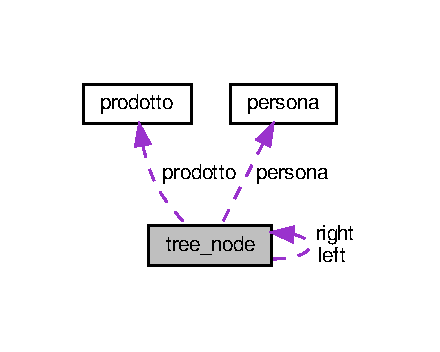
\includegraphics[width=211pt]{structtree__node__coll__graph}
\end{center}
\end{figure}
\subsection*{Data Fields}
\begin{DoxyCompactItemize}
\item 
\hyperlink{head__strutture_8h_afec16ee1fceb6c05f4be3538f36b1997}{prodotto\+\_\+t} $\ast$ \hyperlink{structtree__node_adf54e2cdcc96af8fa0e24eac862bf849}{prodotto}
\item 
\hyperlink{head__strutture_8h_a58439881922e3f6e7ed51e352f2a0c1c}{persona\+\_\+t} $\ast$ \hyperlink{structtree__node_a8aa6034178fc4abc1453c134519d0b92}{persona}
\item 
struct \hyperlink{structtree__node}{tree\+\_\+node} $\ast$ \hyperlink{structtree__node_a3e30a7ba2a4e3286ec7394ba920f2893}{left}
\item 
struct \hyperlink{structtree__node}{tree\+\_\+node} $\ast$ \hyperlink{structtree__node_a6d9a8d8aacc3caada9aed8e308c490a0}{right}
\end{DoxyCompactItemize}


\subsection{Detailed Description}
Struttura dati tree\+\_\+noode.~\newline
Definisce un nodo di un albero binario.~\newline
Puo\textquotesingle{} essere usato sia per le strutture prodotti che per quelle persona, per questo e\textquotesingle{} presente un componente per ciascuno. 

\subsection{Field Documentation}
\mbox{\Hypertarget{structtree__node_a3e30a7ba2a4e3286ec7394ba920f2893}\label{structtree__node_a3e30a7ba2a4e3286ec7394ba920f2893}} 
\index{tree\+\_\+node@{tree\+\_\+node}!left@{left}}
\index{left@{left}!tree\+\_\+node@{tree\+\_\+node}}
\subsubsection{\texorpdfstring{left}{left}}
{\footnotesize\ttfamily struct \hyperlink{structtree__node}{tree\+\_\+node}$\ast$ tree\+\_\+node\+::left}

\mbox{\Hypertarget{structtree__node_a8aa6034178fc4abc1453c134519d0b92}\label{structtree__node_a8aa6034178fc4abc1453c134519d0b92}} 
\index{tree\+\_\+node@{tree\+\_\+node}!persona@{persona}}
\index{persona@{persona}!tree\+\_\+node@{tree\+\_\+node}}
\subsubsection{\texorpdfstring{persona}{persona}}
{\footnotesize\ttfamily \hyperlink{head__strutture_8h_a58439881922e3f6e7ed51e352f2a0c1c}{persona\+\_\+t}$\ast$ tree\+\_\+node\+::persona}

\mbox{\Hypertarget{structtree__node_adf54e2cdcc96af8fa0e24eac862bf849}\label{structtree__node_adf54e2cdcc96af8fa0e24eac862bf849}} 
\index{tree\+\_\+node@{tree\+\_\+node}!prodotto@{prodotto}}
\index{prodotto@{prodotto}!tree\+\_\+node@{tree\+\_\+node}}
\subsubsection{\texorpdfstring{prodotto}{prodotto}}
{\footnotesize\ttfamily \hyperlink{head__strutture_8h_afec16ee1fceb6c05f4be3538f36b1997}{prodotto\+\_\+t}$\ast$ tree\+\_\+node\+::prodotto}

\mbox{\Hypertarget{structtree__node_a6d9a8d8aacc3caada9aed8e308c490a0}\label{structtree__node_a6d9a8d8aacc3caada9aed8e308c490a0}} 
\index{tree\+\_\+node@{tree\+\_\+node}!right@{right}}
\index{right@{right}!tree\+\_\+node@{tree\+\_\+node}}
\subsubsection{\texorpdfstring{right}{right}}
{\footnotesize\ttfamily struct \hyperlink{structtree__node}{tree\+\_\+node}$\ast$ tree\+\_\+node\+::right}



The documentation for this struct was generated from the following file\+:\begin{DoxyCompactItemize}
\item 
src/\hyperlink{head__strutture_8h}{head\+\_\+strutture.\+h}\end{DoxyCompactItemize}

\chapter{File Documentation}
\hypertarget{file_8c}{}\section{src/file.c File Reference}
\label{file_8c}\index{src/file.\+c@{src/file.\+c}}
{\ttfamily \#include \char`\"{}head\+\_\+file.\+h\char`\"{}}\newline
Include dependency graph for file.\+c\+:
\nopagebreak
\begin{figure}[H]
\begin{center}
\leavevmode
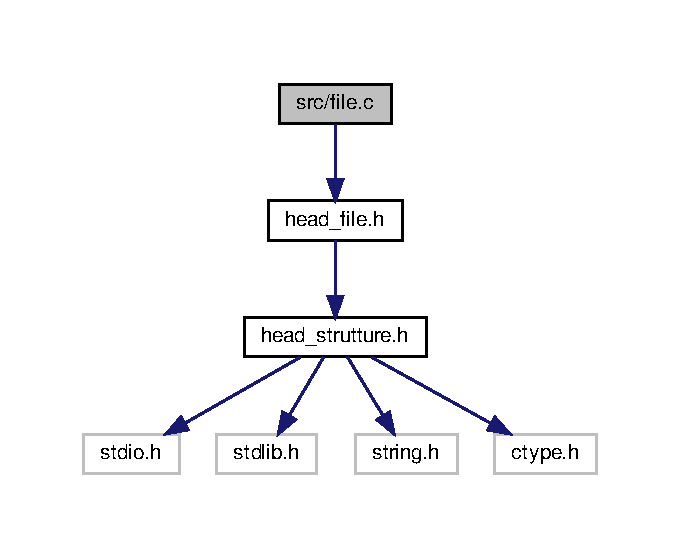
\includegraphics[width=327pt]{file_8c__incl}
\end{center}
\end{figure}
\subsection*{Functions}
\begin{DoxyCompactItemize}
\item 
void \hyperlink{file_8c_abcf6f805e23071ed8a53cae67fdc5624}{print\+\_\+novita} ()
\begin{DoxyCompactList}\small\item\em Stampa il contenuto del file novita.\+txt. \end{DoxyCompactList}\item 
void \hyperlink{file_8c_a3eda9b57c390f964b4e4b89ffb7d1a35}{set\+\_\+novita} ()
\begin{DoxyCompactList}\small\item\em Salvascrive il messaggio inserito al posto di quello presente nel file novita.\+txt. \end{DoxyCompactList}\item 
void \hyperlink{file_8c_a4e7268c1826c7fcc6c3d2a015aae12ed}{insert\+\_\+record\+\_\+default} ()
\begin{DoxyCompactList}\small\item\em Inserisce il record di default nel file dipendenti.\+txt. \end{DoxyCompactList}\item 
int \hyperlink{file_8c_a5207d9f8ca4c9414d70a1a107c15a074}{find\+\_\+row\+\_\+prodotti} (F\+I\+LE $\ast$fp, unsigned long \hyperlink{head__strutture_8h_a20f710d6a73f95164e79b59ee0b883c2a280d7329079c73a4a5df3f35697b60b1}{id}, int $\ast$out)
\begin{DoxyCompactList}\small\item\em Ritorna il numero di riga del record con quell\textquotesingle{}id all\textquotesingle{}interno del file prodotti.\+txt, inoltre imposta out secondo la logica dei metodi creati. \end{DoxyCompactList}\item 
int \hyperlink{file_8c_a0ed14bc8df2b4893cd90b8c112b06adc}{find\+\_\+row\+\_\+persone} (F\+I\+LE $\ast$fp, unsigned int \hyperlink{head__strutture_8h_a20f710d6a73f95164e79b59ee0b883c2a280d7329079c73a4a5df3f35697b60b1}{id}, int $\ast$out)
\begin{DoxyCompactList}\small\item\em Ritorna il numero di riga del record con quell\textquotesingle{}id all\textquotesingle{}interno del file clienti.\+txt o dipendenti.\+txt in base al file passato, inoltre imposta out secondo la logica dei metodi creati. \end{DoxyCompactList}\item 
unsigned long \hyperlink{file_8c_ae03148a8be7cfb76c6296ab64bb8d921}{find\+\_\+next\+\_\+id\+\_\+prodotti} (F\+I\+LE $\ast$fp)
\begin{DoxyCompactList}\small\item\em Ritorna il primo id disponibile in ordine numerico all\textquotesingle{}interno del file prodotti.\+txt. \end{DoxyCompactList}\item 
unsigned int \hyperlink{file_8c_a9a6f0381fb8e1e47262b74bb4199c3a2}{find\+\_\+next\+\_\+id\+\_\+persone} (F\+I\+LE $\ast$fp)
\begin{DoxyCompactList}\small\item\em Ritorna il primo id disponibile in ordine numerico all\textquotesingle{}interno del file clienti.\+txt o dipendenti.\+txt in base al file passato come argomento. \end{DoxyCompactList}\item 
int \hyperlink{file_8c_a633ad1a19377632e8b75c215e05d7f86}{insert\+\_\+record} (\hyperlink{head__strutture_8h_ad83512da590021d7b336c3cb314dc228}{tipofile\+\_\+t} tipo)
\begin{DoxyCompactList}\small\item\em Inserisce il record nel file specificato. \end{DoxyCompactList}\item 
int \hyperlink{file_8c_aadcfa90a0a3a8c38767a9574e37d5350}{delete\+\_\+record} (\hyperlink{head__strutture_8h_ad83512da590021d7b336c3cb314dc228}{tipofile\+\_\+t} tipo)
\begin{DoxyCompactList}\small\item\em Elimina il record dal file specificato se esiste. \end{DoxyCompactList}\item 
int \hyperlink{file_8c_a2aa3a964e04c25e8c44ddb829d9ccc9d}{edit\+\_\+record} (\hyperlink{head__strutture_8h_ad83512da590021d7b336c3cb314dc228}{tipofile\+\_\+t} tipo)
\begin{DoxyCompactList}\small\item\em Modifica il record dal file specificato se esiste. \end{DoxyCompactList}\item 
int \hyperlink{file_8c_abf9633780cee7fef5c815bc604f6b7e1}{match\+\_\+access} (unsigned int \hyperlink{head__strutture_8h_a20f710d6a73f95164e79b59ee0b883c2a280d7329079c73a4a5df3f35697b60b1}{id}, char $\ast$psw)
\begin{DoxyCompactList}\small\item\em Controlla se i dati passati come parametri corrispondono a un record nel file dipendenti.\+txt. \end{DoxyCompactList}\item 
int \hyperlink{file_8c_aa422b9e44e491933e54ce77d24b87f89}{incremental\+\_\+add\+\_\+prodotti} ()
\begin{DoxyCompactList}\small\item\em Incrementa o diminuisce il campo quantita\textquotesingle{} del record con l\textquotesingle{}ID specificato, se esiste. \end{DoxyCompactList}\end{DoxyCompactItemize}


\subsection{Detailed Description}
Contiene i metodi inerenti alla gestione dei file e alcuni metodi utili per l\textquotesingle{}input di stringhe. 

\subsection{Function Documentation}
\mbox{\Hypertarget{file_8c_aadcfa90a0a3a8c38767a9574e37d5350}\label{file_8c_aadcfa90a0a3a8c38767a9574e37d5350}} 
\index{file.\+c@{file.\+c}!delete\+\_\+record@{delete\+\_\+record}}
\index{delete\+\_\+record@{delete\+\_\+record}!file.\+c@{file.\+c}}
\subsubsection{\texorpdfstring{delete\+\_\+record()}{delete\_record()}}
{\footnotesize\ttfamily int delete\+\_\+record (\begin{DoxyParamCaption}\item[{\hyperlink{head__strutture_8h_ad83512da590021d7b336c3cb314dc228}{tipofile\+\_\+t}}]{tipo }\end{DoxyParamCaption})}



Elimina il record dal file specificato se esiste. 

In base al file specificato dal parametro d\textquotesingle{}ingresso, visualizza l\textquotesingle{}interfaccia grafica per inserire i dati dei record e se i dati inseriti sono consistenti elimina dal file giusto il record con l\textquotesingle{}ID inserito.~\newline
Ritorna 0 se la cancellazione e\textquotesingle{} avvenuta con successo, -\/1 se i dati inseriti sono inconsistenti o non e\textquotesingle{} stato possibile trovare il record con l\textquotesingle{}ID inserito.~\newline
Se i file non esistono, questi verranno automaticamente creati.~\newline
Inserisce il record di default se necessario nel file dipendenti.\+txt. 
\begin{DoxyParams}{Parameters}
{\em tipofile\+\_\+t} & tipo \\
\hline
\end{DoxyParams}
\begin{DoxyReturn}{Returns}
int 
\end{DoxyReturn}
\mbox{\Hypertarget{file_8c_a2aa3a964e04c25e8c44ddb829d9ccc9d}\label{file_8c_a2aa3a964e04c25e8c44ddb829d9ccc9d}} 
\index{file.\+c@{file.\+c}!edit\+\_\+record@{edit\+\_\+record}}
\index{edit\+\_\+record@{edit\+\_\+record}!file.\+c@{file.\+c}}
\subsubsection{\texorpdfstring{edit\+\_\+record()}{edit\_record()}}
{\footnotesize\ttfamily int edit\+\_\+record (\begin{DoxyParamCaption}\item[{\hyperlink{head__strutture_8h_ad83512da590021d7b336c3cb314dc228}{tipofile\+\_\+t}}]{tipo }\end{DoxyParamCaption})}



Modifica il record dal file specificato se esiste. 

In base al file specificato dal parametro d\textquotesingle{}ingresso, visualizza l\textquotesingle{}interfaccia grafica per inserire i dati dei record e se i dati inseriti sono consistenti modifica nel file giusto il record con l\textquotesingle{}ID inserito.~\newline
Ritorna 0 se la modifica e\textquotesingle{} avvenuta con successo, -\/1 se i dati inseriti sono inconsistenti o non e\textquotesingle{} stato possibile trovare il record con l\textquotesingle{}ID inserito.~\newline
Se i file non esistono, questi verranno automaticamente creati.~\newline
Inserisce il record di default se necessario nel file dipendenti.\+txt. 
\begin{DoxyParams}{Parameters}
{\em tipofile\+\_\+t} & tipo \\
\hline
\end{DoxyParams}
\begin{DoxyReturn}{Returns}
int 
\end{DoxyReturn}
\mbox{\Hypertarget{file_8c_a9a6f0381fb8e1e47262b74bb4199c3a2}\label{file_8c_a9a6f0381fb8e1e47262b74bb4199c3a2}} 
\index{file.\+c@{file.\+c}!find\+\_\+next\+\_\+id\+\_\+persone@{find\+\_\+next\+\_\+id\+\_\+persone}}
\index{find\+\_\+next\+\_\+id\+\_\+persone@{find\+\_\+next\+\_\+id\+\_\+persone}!file.\+c@{file.\+c}}
\subsubsection{\texorpdfstring{find\+\_\+next\+\_\+id\+\_\+persone()}{find\_next\_id\_persone()}}
{\footnotesize\ttfamily unsigned int find\+\_\+next\+\_\+id\+\_\+persone (\begin{DoxyParamCaption}\item[{F\+I\+LE $\ast$}]{fp }\end{DoxyParamCaption})}



Ritorna il primo id disponibile in ordine numerico all\textquotesingle{}interno del file clienti.\+txt o dipendenti.\+txt in base al file passato come argomento. 


\begin{DoxyParams}{Parameters}
{\em F\+I\+LE} & $\ast$file \\
\hline
\end{DoxyParams}
\begin{DoxyReturn}{Returns}
unsigned int 
\end{DoxyReturn}
\mbox{\Hypertarget{file_8c_ae03148a8be7cfb76c6296ab64bb8d921}\label{file_8c_ae03148a8be7cfb76c6296ab64bb8d921}} 
\index{file.\+c@{file.\+c}!find\+\_\+next\+\_\+id\+\_\+prodotti@{find\+\_\+next\+\_\+id\+\_\+prodotti}}
\index{find\+\_\+next\+\_\+id\+\_\+prodotti@{find\+\_\+next\+\_\+id\+\_\+prodotti}!file.\+c@{file.\+c}}
\subsubsection{\texorpdfstring{find\+\_\+next\+\_\+id\+\_\+prodotti()}{find\_next\_id\_prodotti()}}
{\footnotesize\ttfamily unsigned long find\+\_\+next\+\_\+id\+\_\+prodotti (\begin{DoxyParamCaption}\item[{F\+I\+LE $\ast$}]{fp }\end{DoxyParamCaption})}



Ritorna il primo id disponibile in ordine numerico all\textquotesingle{}interno del file prodotti.\+txt. 


\begin{DoxyParams}{Parameters}
{\em F\+I\+LE} & $\ast$file \\
\hline
\end{DoxyParams}
\begin{DoxyReturn}{Returns}
unsigned long 
\end{DoxyReturn}
\mbox{\Hypertarget{file_8c_a0ed14bc8df2b4893cd90b8c112b06adc}\label{file_8c_a0ed14bc8df2b4893cd90b8c112b06adc}} 
\index{file.\+c@{file.\+c}!find\+\_\+row\+\_\+persone@{find\+\_\+row\+\_\+persone}}
\index{find\+\_\+row\+\_\+persone@{find\+\_\+row\+\_\+persone}!file.\+c@{file.\+c}}
\subsubsection{\texorpdfstring{find\+\_\+row\+\_\+persone()}{find\_row\_persone()}}
{\footnotesize\ttfamily int find\+\_\+row\+\_\+persone (\begin{DoxyParamCaption}\item[{F\+I\+LE $\ast$}]{fp,  }\item[{unsigned int}]{id,  }\item[{int $\ast$}]{out }\end{DoxyParamCaption})}



Ritorna il numero di riga del record con quell\textquotesingle{}id all\textquotesingle{}interno del file clienti.\+txt o dipendenti.\+txt in base al file passato, inoltre imposta out secondo la logica dei metodi creati. 


\begin{DoxyParams}{Parameters}
{\em F\+I\+LE} & $\ast$file \\
\hline
{\em unsigned} & int id \\
\hline
{\em int} & $\ast$out \\
\hline
\end{DoxyParams}
\begin{DoxyReturn}{Returns}
int 
\end{DoxyReturn}
\mbox{\Hypertarget{file_8c_a5207d9f8ca4c9414d70a1a107c15a074}\label{file_8c_a5207d9f8ca4c9414d70a1a107c15a074}} 
\index{file.\+c@{file.\+c}!find\+\_\+row\+\_\+prodotti@{find\+\_\+row\+\_\+prodotti}}
\index{find\+\_\+row\+\_\+prodotti@{find\+\_\+row\+\_\+prodotti}!file.\+c@{file.\+c}}
\subsubsection{\texorpdfstring{find\+\_\+row\+\_\+prodotti()}{find\_row\_prodotti()}}
{\footnotesize\ttfamily int find\+\_\+row\+\_\+prodotti (\begin{DoxyParamCaption}\item[{F\+I\+LE $\ast$}]{fp,  }\item[{unsigned long}]{id,  }\item[{int $\ast$}]{out }\end{DoxyParamCaption})}



Ritorna il numero di riga del record con quell\textquotesingle{}id all\textquotesingle{}interno del file prodotti.\+txt, inoltre imposta out secondo la logica dei metodi creati. 


\begin{DoxyParams}{Parameters}
{\em F\+I\+LE} & $\ast$file \\
\hline
{\em unsigned} & long id \\
\hline
{\em int} & $\ast$out \\
\hline
\end{DoxyParams}
\begin{DoxyReturn}{Returns}
int 
\end{DoxyReturn}
\mbox{\Hypertarget{file_8c_aa422b9e44e491933e54ce77d24b87f89}\label{file_8c_aa422b9e44e491933e54ce77d24b87f89}} 
\index{file.\+c@{file.\+c}!incremental\+\_\+add\+\_\+prodotti@{incremental\+\_\+add\+\_\+prodotti}}
\index{incremental\+\_\+add\+\_\+prodotti@{incremental\+\_\+add\+\_\+prodotti}!file.\+c@{file.\+c}}
\subsubsection{\texorpdfstring{incremental\+\_\+add\+\_\+prodotti()}{incremental\_add\_prodotti()}}
{\footnotesize\ttfamily int incremental\+\_\+add\+\_\+prodotti (\begin{DoxyParamCaption}{ }\end{DoxyParamCaption})}



Incrementa o diminuisce il campo quantita\textquotesingle{} del record con l\textquotesingle{}ID specificato, se esiste. 

Non si puo\textquotesingle{} decrementare piu\textquotesingle{} di quello che c\textquotesingle{}e\textquotesingle{} in magazzino, se si fa\textquotesingle{}, il record non viene modificato e compare un messaggio di errore.~\newline
Se il file prodotti.\+txt non esiste viene creato automaticamente.~\newline
Ritorna 0 se la modifica e\textquotesingle{} avvenuta correttamente, -\/1 se si e\textquotesingle{} tentato di decrementare piu\textquotesingle{} di quanto consentito, o i dati inseriti sono inconsistenti. \begin{DoxyReturn}{Returns}
int 
\end{DoxyReturn}
\mbox{\Hypertarget{file_8c_a633ad1a19377632e8b75c215e05d7f86}\label{file_8c_a633ad1a19377632e8b75c215e05d7f86}} 
\index{file.\+c@{file.\+c}!insert\+\_\+record@{insert\+\_\+record}}
\index{insert\+\_\+record@{insert\+\_\+record}!file.\+c@{file.\+c}}
\subsubsection{\texorpdfstring{insert\+\_\+record()}{insert\_record()}}
{\footnotesize\ttfamily int insert\+\_\+record (\begin{DoxyParamCaption}\item[{\hyperlink{head__strutture_8h_ad83512da590021d7b336c3cb314dc228}{tipofile\+\_\+t}}]{tipo }\end{DoxyParamCaption})}



Inserisce il record nel file specificato. 

In base al file specificato dal parametro d\textquotesingle{}ingresso, visualizza l\textquotesingle{}interfaccia grafica per inserire i dati dei record e se i dati inseriti sono consistenti inserisce nel file giusto il record in ordine numerico col primo ID disponibile.~\newline
Ritorna 0 se l\textquotesingle{}inserimento e\textquotesingle{} avvenuto con successo, -\/1 se i dati inseriti sono inconsistenti o non e\textquotesingle{} stato possibile inserire il record nel file.~\newline
Se i file non esistono, questi verranno automaticamente creati./n A\+T\+T\+E\+N\+Z\+I\+O\+NE\+: Questo metodo non aggiunge il record di default al file dipendenti.\+txt, in questo modo e\textquotesingle{} possibile aggiungere il record 1 se prima si ha cancellato il record di default. 
\begin{DoxyParams}{Parameters}
{\em tipofile\+\_\+t} & tipo \\
\hline
\end{DoxyParams}
\begin{DoxyReturn}{Returns}
int 
\end{DoxyReturn}
\mbox{\Hypertarget{file_8c_a4e7268c1826c7fcc6c3d2a015aae12ed}\label{file_8c_a4e7268c1826c7fcc6c3d2a015aae12ed}} 
\index{file.\+c@{file.\+c}!insert\+\_\+record\+\_\+default@{insert\+\_\+record\+\_\+default}}
\index{insert\+\_\+record\+\_\+default@{insert\+\_\+record\+\_\+default}!file.\+c@{file.\+c}}
\subsubsection{\texorpdfstring{insert\+\_\+record\+\_\+default()}{insert\_record\_default()}}
{\footnotesize\ttfamily void insert\+\_\+record\+\_\+default (\begin{DoxyParamCaption}{ }\end{DoxyParamCaption})}



Inserisce il record di default nel file dipendenti.\+txt. 

\mbox{\Hypertarget{file_8c_abf9633780cee7fef5c815bc604f6b7e1}\label{file_8c_abf9633780cee7fef5c815bc604f6b7e1}} 
\index{file.\+c@{file.\+c}!match\+\_\+access@{match\+\_\+access}}
\index{match\+\_\+access@{match\+\_\+access}!file.\+c@{file.\+c}}
\subsubsection{\texorpdfstring{match\+\_\+access()}{match\_access()}}
{\footnotesize\ttfamily int match\+\_\+access (\begin{DoxyParamCaption}\item[{unsigned int}]{id,  }\item[{char $\ast$}]{psw }\end{DoxyParamCaption})}



Controlla se i dati passati come parametri corrispondono a un record nel file dipendenti.\+txt. 

Se il file dipendenti.\+txt non esiste, questo verra\textquotesingle{} automaticamente creato, inoltre verra\textquotesingle{} inserito il record di default. Ritorna 0 se c\textquotesingle{}e\textquotesingle{} stato un match, altrimenti ritorna -\/1.~\newline
Inserisce il record di default se necessario nel file dipendenti.\+txt. 
\begin{DoxyParams}{Parameters}
{\em unsigned} & int id \\
\hline
{\em char} & $\ast$psw \\
\hline
\end{DoxyParams}
\begin{DoxyReturn}{Returns}
int 
\end{DoxyReturn}
\mbox{\Hypertarget{file_8c_abcf6f805e23071ed8a53cae67fdc5624}\label{file_8c_abcf6f805e23071ed8a53cae67fdc5624}} 
\index{file.\+c@{file.\+c}!print\+\_\+novita@{print\+\_\+novita}}
\index{print\+\_\+novita@{print\+\_\+novita}!file.\+c@{file.\+c}}
\subsubsection{\texorpdfstring{print\+\_\+novita()}{print\_novita()}}
{\footnotesize\ttfamily void print\+\_\+novita (\begin{DoxyParamCaption}{ }\end{DoxyParamCaption})}



Stampa il contenuto del file novita.\+txt. 

\mbox{\Hypertarget{file_8c_a3eda9b57c390f964b4e4b89ffb7d1a35}\label{file_8c_a3eda9b57c390f964b4e4b89ffb7d1a35}} 
\index{file.\+c@{file.\+c}!set\+\_\+novita@{set\+\_\+novita}}
\index{set\+\_\+novita@{set\+\_\+novita}!file.\+c@{file.\+c}}
\subsubsection{\texorpdfstring{set\+\_\+novita()}{set\_novita()}}
{\footnotesize\ttfamily void set\+\_\+novita (\begin{DoxyParamCaption}{ }\end{DoxyParamCaption})}



Salvascrive il messaggio inserito al posto di quello presente nel file novita.\+txt. 

Il messaggio deve essere lungo al massimo 400 caratteri (e\textquotesingle{} escluso il carattere $\sim$).~\newline
Il messaggio viene considerato fino al carattere $\sim$ o fino a quando non si e\textquotesingle{} raggiunto i 400 caratteri.~\newline
Il messaggio viene salvascritto solo se si inserisce qualcosa oltre al simbolo $\sim$ . 
\hypertarget{head__file_8h}{}\section{src/head\+\_\+file.h File Reference}
\label{head__file_8h}\index{src/head\+\_\+file.\+h@{src/head\+\_\+file.\+h}}
{\ttfamily \#include \char`\"{}head\+\_\+strutture.\+h\char`\"{}}\newline
Include dependency graph for head\+\_\+file.\+h\+:
\nopagebreak
\begin{figure}[H]
\begin{center}
\leavevmode
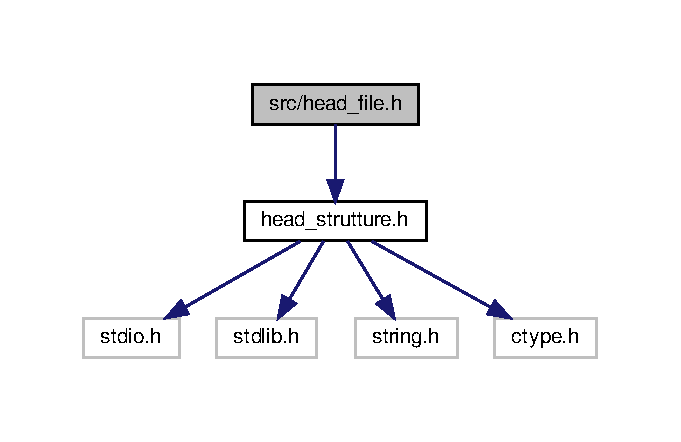
\includegraphics[width=327pt]{head__file_8h__incl}
\end{center}
\end{figure}
This graph shows which files directly or indirectly include this file\+:
\nopagebreak
\begin{figure}[H]
\begin{center}
\leavevmode
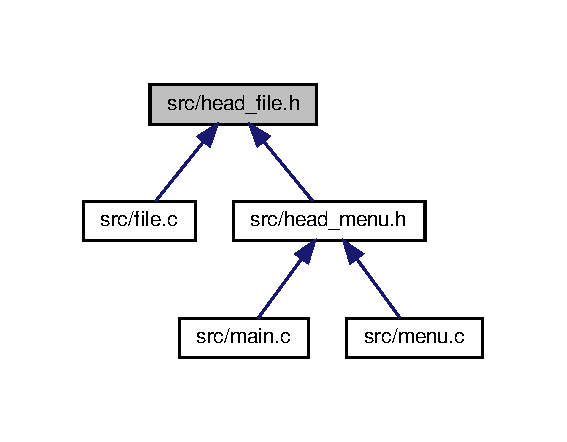
\includegraphics[width=272pt]{head__file_8h__dep__incl}
\end{center}
\end{figure}
\subsection*{Functions}
\begin{DoxyCompactItemize}
\item 
void \hyperlink{head__file_8h_a4e7268c1826c7fcc6c3d2a015aae12ed}{insert\+\_\+record\+\_\+default} ()
\begin{DoxyCompactList}\small\item\em Inserisce il record di default nel file dipendenti.\+txt. \end{DoxyCompactList}\item 
int \hyperlink{head__file_8h_abf9633780cee7fef5c815bc604f6b7e1}{match\+\_\+access} (unsigned int \hyperlink{head__strutture_8h_a20f710d6a73f95164e79b59ee0b883c2a280d7329079c73a4a5df3f35697b60b1}{id}, char $\ast$psw)
\begin{DoxyCompactList}\small\item\em Controlla se i dati passati come parametri corrispondono a un record nel file dipendenti.\+txt. \end{DoxyCompactList}\item 
int \hyperlink{head__file_8h_a633ad1a19377632e8b75c215e05d7f86}{insert\+\_\+record} (\hyperlink{head__strutture_8h_ad83512da590021d7b336c3cb314dc228}{tipofile\+\_\+t} tipo)
\begin{DoxyCompactList}\small\item\em Inserisce il record nel file specificato. \end{DoxyCompactList}\item 
int \hyperlink{head__file_8h_aadcfa90a0a3a8c38767a9574e37d5350}{delete\+\_\+record} (\hyperlink{head__strutture_8h_ad83512da590021d7b336c3cb314dc228}{tipofile\+\_\+t} tipo)
\begin{DoxyCompactList}\small\item\em Elimina il record dal file specificato se esiste. \end{DoxyCompactList}\item 
int \hyperlink{head__file_8h_a2aa3a964e04c25e8c44ddb829d9ccc9d}{edit\+\_\+record} (\hyperlink{head__strutture_8h_ad83512da590021d7b336c3cb314dc228}{tipofile\+\_\+t} tipo)
\begin{DoxyCompactList}\small\item\em Modifica il record dal file specificato se esiste. \end{DoxyCompactList}\item 
void \hyperlink{head__file_8h_abcf6f805e23071ed8a53cae67fdc5624}{print\+\_\+novita} ()
\begin{DoxyCompactList}\small\item\em Stampa il contenuto del file novita.\+txt. \end{DoxyCompactList}\item 
void \hyperlink{head__file_8h_a3eda9b57c390f964b4e4b89ffb7d1a35}{set\+\_\+novita} ()
\begin{DoxyCompactList}\small\item\em Salvascrive il messaggio inserito al posto di quello presente nel file novita.\+txt. \end{DoxyCompactList}\item 
int \hyperlink{head__file_8h_aa422b9e44e491933e54ce77d24b87f89}{incremental\+\_\+add\+\_\+prodotti} ()
\begin{DoxyCompactList}\small\item\em Incrementa o diminuisce il campo quantita\textquotesingle{} del record con l\textquotesingle{}ID specificato, se esiste. \end{DoxyCompactList}\end{DoxyCompactItemize}


\subsection{Detailed Description}
Contiene le definizioni dei metodi che potrebbero essere usati da altri file. 

\subsection{Function Documentation}
\mbox{\Hypertarget{head__file_8h_aadcfa90a0a3a8c38767a9574e37d5350}\label{head__file_8h_aadcfa90a0a3a8c38767a9574e37d5350}} 
\index{head\+\_\+file.\+h@{head\+\_\+file.\+h}!delete\+\_\+record@{delete\+\_\+record}}
\index{delete\+\_\+record@{delete\+\_\+record}!head\+\_\+file.\+h@{head\+\_\+file.\+h}}
\subsubsection{\texorpdfstring{delete\+\_\+record()}{delete\_record()}}
{\footnotesize\ttfamily int delete\+\_\+record (\begin{DoxyParamCaption}\item[{\hyperlink{head__strutture_8h_ad83512da590021d7b336c3cb314dc228}{tipofile\+\_\+t}}]{tipo }\end{DoxyParamCaption})}



Elimina il record dal file specificato se esiste. 

In base al file specificato dal parametro d\textquotesingle{}ingresso, visualizza l\textquotesingle{}interfaccia grafica per inserire i dati dei record e se i dati inseriti sono consistenti elimina dal file giusto il record con l\textquotesingle{}ID inserito.~\newline
Ritorna 0 se la cancellazione e\textquotesingle{} avvenuta con successo, -\/1 se i dati inseriti sono inconsistenti o non e\textquotesingle{} stato possibile trovare il record con l\textquotesingle{}ID inserito.~\newline
Se i file non esistono, questi verranno automaticamente creati.~\newline
Inserisce il record di default se necessario nel file dipendenti.\+txt. 
\begin{DoxyParams}{Parameters}
{\em tipofile\+\_\+t} & tipo \\
\hline
\end{DoxyParams}
\begin{DoxyReturn}{Returns}
int 
\end{DoxyReturn}
\mbox{\Hypertarget{head__file_8h_a2aa3a964e04c25e8c44ddb829d9ccc9d}\label{head__file_8h_a2aa3a964e04c25e8c44ddb829d9ccc9d}} 
\index{head\+\_\+file.\+h@{head\+\_\+file.\+h}!edit\+\_\+record@{edit\+\_\+record}}
\index{edit\+\_\+record@{edit\+\_\+record}!head\+\_\+file.\+h@{head\+\_\+file.\+h}}
\subsubsection{\texorpdfstring{edit\+\_\+record()}{edit\_record()}}
{\footnotesize\ttfamily int edit\+\_\+record (\begin{DoxyParamCaption}\item[{\hyperlink{head__strutture_8h_ad83512da590021d7b336c3cb314dc228}{tipofile\+\_\+t}}]{tipo }\end{DoxyParamCaption})}



Modifica il record dal file specificato se esiste. 

In base al file specificato dal parametro d\textquotesingle{}ingresso, visualizza l\textquotesingle{}interfaccia grafica per inserire i dati dei record e se i dati inseriti sono consistenti modifica nel file giusto il record con l\textquotesingle{}ID inserito.~\newline
Ritorna 0 se la modifica e\textquotesingle{} avvenuta con successo, -\/1 se i dati inseriti sono inconsistenti o non e\textquotesingle{} stato possibile trovare il record con l\textquotesingle{}ID inserito.~\newline
Se i file non esistono, questi verranno automaticamente creati.~\newline
Inserisce il record di default se necessario nel file dipendenti.\+txt. 
\begin{DoxyParams}{Parameters}
{\em tipofile\+\_\+t} & tipo \\
\hline
\end{DoxyParams}
\begin{DoxyReturn}{Returns}
int 
\end{DoxyReturn}
\mbox{\Hypertarget{head__file_8h_aa422b9e44e491933e54ce77d24b87f89}\label{head__file_8h_aa422b9e44e491933e54ce77d24b87f89}} 
\index{head\+\_\+file.\+h@{head\+\_\+file.\+h}!incremental\+\_\+add\+\_\+prodotti@{incremental\+\_\+add\+\_\+prodotti}}
\index{incremental\+\_\+add\+\_\+prodotti@{incremental\+\_\+add\+\_\+prodotti}!head\+\_\+file.\+h@{head\+\_\+file.\+h}}
\subsubsection{\texorpdfstring{incremental\+\_\+add\+\_\+prodotti()}{incremental\_add\_prodotti()}}
{\footnotesize\ttfamily int incremental\+\_\+add\+\_\+prodotti (\begin{DoxyParamCaption}{ }\end{DoxyParamCaption})}



Incrementa o diminuisce il campo quantita\textquotesingle{} del record con l\textquotesingle{}ID specificato, se esiste. 

Non si puo\textquotesingle{} decrementare piu\textquotesingle{} di quello che c\textquotesingle{}e\textquotesingle{} in magazzino, se si fa\textquotesingle{}, il record non viene modificato e compare un messaggio di errore.~\newline
Se il file prodotti.\+txt non esiste viene creato automaticamente.~\newline
Ritorna 0 se la modifica e\textquotesingle{} avvenuta correttamente, -\/1 se si e\textquotesingle{} tentato di decrementare piu\textquotesingle{} di quanto consentito, o i dati inseriti sono inconsistenti. \begin{DoxyReturn}{Returns}
int 
\end{DoxyReturn}
\mbox{\Hypertarget{head__file_8h_a633ad1a19377632e8b75c215e05d7f86}\label{head__file_8h_a633ad1a19377632e8b75c215e05d7f86}} 
\index{head\+\_\+file.\+h@{head\+\_\+file.\+h}!insert\+\_\+record@{insert\+\_\+record}}
\index{insert\+\_\+record@{insert\+\_\+record}!head\+\_\+file.\+h@{head\+\_\+file.\+h}}
\subsubsection{\texorpdfstring{insert\+\_\+record()}{insert\_record()}}
{\footnotesize\ttfamily int insert\+\_\+record (\begin{DoxyParamCaption}\item[{\hyperlink{head__strutture_8h_ad83512da590021d7b336c3cb314dc228}{tipofile\+\_\+t}}]{tipo }\end{DoxyParamCaption})}



Inserisce il record nel file specificato. 

In base al file specificato dal parametro d\textquotesingle{}ingresso, visualizza l\textquotesingle{}interfaccia grafica per inserire i dati dei record e se i dati inseriti sono consistenti inserisce nel file giusto il record in ordine numerico col primo ID disponibile.~\newline
Ritorna 0 se l\textquotesingle{}inserimento e\textquotesingle{} avvenuto con successo, -\/1 se i dati inseriti sono inconsistenti o non e\textquotesingle{} stato possibile inserire il record nel file.~\newline
Se i file non esistono, questi verranno automaticamente creati./n A\+T\+T\+E\+N\+Z\+I\+O\+NE\+: Questo metodo non aggiunge il record di default al file dipendenti.\+txt, in questo modo e\textquotesingle{} possibile aggiungere il record 1 se prima si ha cancellato il record di default. 
\begin{DoxyParams}{Parameters}
{\em tipofile\+\_\+t} & tipo \\
\hline
\end{DoxyParams}
\begin{DoxyReturn}{Returns}
int 
\end{DoxyReturn}
\mbox{\Hypertarget{head__file_8h_a4e7268c1826c7fcc6c3d2a015aae12ed}\label{head__file_8h_a4e7268c1826c7fcc6c3d2a015aae12ed}} 
\index{head\+\_\+file.\+h@{head\+\_\+file.\+h}!insert\+\_\+record\+\_\+default@{insert\+\_\+record\+\_\+default}}
\index{insert\+\_\+record\+\_\+default@{insert\+\_\+record\+\_\+default}!head\+\_\+file.\+h@{head\+\_\+file.\+h}}
\subsubsection{\texorpdfstring{insert\+\_\+record\+\_\+default()}{insert\_record\_default()}}
{\footnotesize\ttfamily void insert\+\_\+record\+\_\+default (\begin{DoxyParamCaption}{ }\end{DoxyParamCaption})}



Inserisce il record di default nel file dipendenti.\+txt. 

\mbox{\Hypertarget{head__file_8h_abf9633780cee7fef5c815bc604f6b7e1}\label{head__file_8h_abf9633780cee7fef5c815bc604f6b7e1}} 
\index{head\+\_\+file.\+h@{head\+\_\+file.\+h}!match\+\_\+access@{match\+\_\+access}}
\index{match\+\_\+access@{match\+\_\+access}!head\+\_\+file.\+h@{head\+\_\+file.\+h}}
\subsubsection{\texorpdfstring{match\+\_\+access()}{match\_access()}}
{\footnotesize\ttfamily int match\+\_\+access (\begin{DoxyParamCaption}\item[{unsigned int}]{id,  }\item[{char $\ast$}]{psw }\end{DoxyParamCaption})}



Controlla se i dati passati come parametri corrispondono a un record nel file dipendenti.\+txt. 

Se il file dipendenti.\+txt non esiste, questo verra\textquotesingle{} automaticamente creato, inoltre verra\textquotesingle{} inserito il record di default. Ritorna 0 se c\textquotesingle{}e\textquotesingle{} stato un match, altrimenti ritorna -\/1.~\newline
Inserisce il record di default se necessario nel file dipendenti.\+txt. 
\begin{DoxyParams}{Parameters}
{\em unsigned} & int id \\
\hline
{\em char} & $\ast$psw \\
\hline
\end{DoxyParams}
\begin{DoxyReturn}{Returns}
int 
\end{DoxyReturn}
\mbox{\Hypertarget{head__file_8h_abcf6f805e23071ed8a53cae67fdc5624}\label{head__file_8h_abcf6f805e23071ed8a53cae67fdc5624}} 
\index{head\+\_\+file.\+h@{head\+\_\+file.\+h}!print\+\_\+novita@{print\+\_\+novita}}
\index{print\+\_\+novita@{print\+\_\+novita}!head\+\_\+file.\+h@{head\+\_\+file.\+h}}
\subsubsection{\texorpdfstring{print\+\_\+novita()}{print\_novita()}}
{\footnotesize\ttfamily void print\+\_\+novita (\begin{DoxyParamCaption}{ }\end{DoxyParamCaption})}



Stampa il contenuto del file novita.\+txt. 

\mbox{\Hypertarget{head__file_8h_a3eda9b57c390f964b4e4b89ffb7d1a35}\label{head__file_8h_a3eda9b57c390f964b4e4b89ffb7d1a35}} 
\index{head\+\_\+file.\+h@{head\+\_\+file.\+h}!set\+\_\+novita@{set\+\_\+novita}}
\index{set\+\_\+novita@{set\+\_\+novita}!head\+\_\+file.\+h@{head\+\_\+file.\+h}}
\subsubsection{\texorpdfstring{set\+\_\+novita()}{set\_novita()}}
{\footnotesize\ttfamily void set\+\_\+novita (\begin{DoxyParamCaption}{ }\end{DoxyParamCaption})}



Salvascrive il messaggio inserito al posto di quello presente nel file novita.\+txt. 

Il messaggio deve essere lungo al massimo 400 caratteri (e\textquotesingle{} escluso il carattere $\sim$).~\newline
Il messaggio viene considerato fino al carattere $\sim$ o fino a quando non si e\textquotesingle{} raggiunto i 400 caratteri.~\newline
Il messaggio viene salvascritto solo se si inserisce qualcosa oltre al simbolo $\sim$ . 
\hypertarget{head__menu_8h}{}\section{src/head\+\_\+menu.h File Reference}
\label{head__menu_8h}\index{src/head\+\_\+menu.\+h@{src/head\+\_\+menu.\+h}}
{\ttfamily \#include \char`\"{}head\+\_\+file.\+h\char`\"{}}\newline
{\ttfamily \#include \char`\"{}head\+\_\+ordinamento.\+h\char`\"{}}\newline
Include dependency graph for head\+\_\+menu.\+h\+:
\nopagebreak
\begin{figure}[H]
\begin{center}
\leavevmode
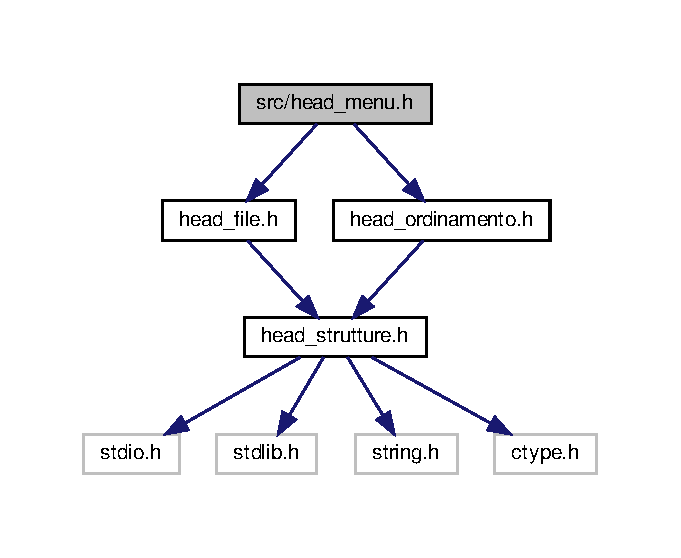
\includegraphics[width=327pt]{head__menu_8h__incl}
\end{center}
\end{figure}
This graph shows which files directly or indirectly include this file\+:
\nopagebreak
\begin{figure}[H]
\begin{center}
\leavevmode
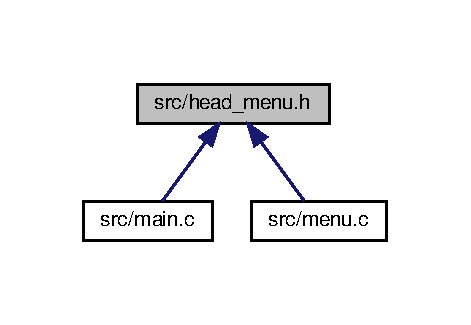
\includegraphics[width=226pt]{head__menu_8h__dep__incl}
\end{center}
\end{figure}
\subsection*{Functions}
\begin{DoxyCompactItemize}
\item 
void \hyperlink{head__menu_8h_aa510a50efd9498c295969cf173fc6337}{show\+\_\+nolog\+\_\+menu} ()
\begin{DoxyCompactList}\small\item\em Mostra l\textquotesingle{}interfaccia grafica del menu\textquotesingle{} nolog. \end{DoxyCompactList}\item 
void \hyperlink{head__menu_8h_a0c94e4af9357a56b13dc6cf246a8fb92}{show\+\_\+log\+\_\+menu} ()
\begin{DoxyCompactList}\small\item\em Mostra l\textquotesingle{}interfaccia grafica del menu\textquotesingle{} log. \end{DoxyCompactList}\item 
void \hyperlink{head__menu_8h_aad25e471acaffe14832ddc5437f41c6d}{show\+\_\+prodotti\+\_\+menu} ()
\begin{DoxyCompactList}\small\item\em Mostra l\textquotesingle{}interfaccia grafica del menu\textquotesingle{} principale prodotti. \end{DoxyCompactList}\item 
void \hyperlink{head__menu_8h_a4f9be92c193bf45a9635e3c00bddc030}{show\+\_\+novita\+\_\+menu} ()
\begin{DoxyCompactList}\small\item\em Mostra l\textquotesingle{}interfaccia grafica del menu\textquotesingle{} principale novita\textquotesingle{}. \end{DoxyCompactList}\item 
void \hyperlink{head__menu_8h_adecccf77072a3787432afbfc4d87c4d8}{show\+\_\+clienti\+\_\+menu} ()
\begin{DoxyCompactList}\small\item\em Mostra l\textquotesingle{}interfaccia grafica del menu\textquotesingle{} principale clienti. \end{DoxyCompactList}\item 
void \hyperlink{head__menu_8h_a92366c9bd30febe9b239551d133525f1}{show\+\_\+dipendenti\+\_\+menu} ()
\begin{DoxyCompactList}\small\item\em Mostra l\textquotesingle{}interfaccia grafica del menu\textquotesingle{} principale dipendenti. \end{DoxyCompactList}\item 
void \hyperlink{head__menu_8h_a6b162ea688a7c5a59e96e8177dfda86d}{show\+\_\+ordinamento\+\_\+prodotti\+\_\+menu} ()
\begin{DoxyCompactList}\small\item\em Mostra l\textquotesingle{}interfaccia grafica del menu\textquotesingle{} per la scelta del tipo di ordinamento per i prodotti. \end{DoxyCompactList}\item 
void \hyperlink{head__menu_8h_ac9b4d8c08fe2a2db50c306d3c150ca28}{show\+\_\+ordinamento\+\_\+persone\+\_\+menu} ()
\begin{DoxyCompactList}\small\item\em Mostra l\textquotesingle{}interfaccia grafica del menu\textquotesingle{} per la scelta del tipo di ordinamento per dipendenti e clienti. \end{DoxyCompactList}\item 
int \hyperlink{head__menu_8h_adceb36f3ebfff88ac2283e19d50c01a6}{choise} (\hyperlink{head__strutture_8h_a27938a0a874a833cfee26456c5d730b1}{menu\+\_\+t} m)
\begin{DoxyCompactList}\small\item\em In base a quale menu\textquotesingle{} e\textquotesingle{} stato appena visualizzato, gestisce l\textquotesingle{}immissione dei possibili input controllandone la consistenza col tipo di menu.~\newline
Ritorna la scelta consistente dell\textquotesingle{}utente. \end{DoxyCompactList}\item 
int \hyperlink{head__menu_8h_a96fb221481623d0f77e6fd1e6f7ad118}{menu\+\_\+nextmove} (\hyperlink{head__strutture_8h_a784ca7b7fa64cbb661eb0c903348c1ce}{sessione\+\_\+t} $\ast$se)
\begin{DoxyCompactList}\small\item\em Imposta la prossima azione del programma. \end{DoxyCompactList}\end{DoxyCompactItemize}


\subsection{Detailed Description}
Contiene le definizioni dei metodi che potrebbero essere usati da altri file~\newline
. In particolare sono presenti i metodi inerenti alla parte di visualizzazione e gestione dei menu. 

\subsection{Function Documentation}
\mbox{\Hypertarget{head__menu_8h_adceb36f3ebfff88ac2283e19d50c01a6}\label{head__menu_8h_adceb36f3ebfff88ac2283e19d50c01a6}} 
\index{head\+\_\+menu.\+h@{head\+\_\+menu.\+h}!choise@{choise}}
\index{choise@{choise}!head\+\_\+menu.\+h@{head\+\_\+menu.\+h}}
\subsubsection{\texorpdfstring{choise()}{choise()}}
{\footnotesize\ttfamily int choise (\begin{DoxyParamCaption}\item[{\hyperlink{head__strutture_8h_a27938a0a874a833cfee26456c5d730b1}{menu\+\_\+t}}]{m }\end{DoxyParamCaption})}



In base a quale menu\textquotesingle{} e\textquotesingle{} stato appena visualizzato, gestisce l\textquotesingle{}immissione dei possibili input controllandone la consistenza col tipo di menu.~\newline
Ritorna la scelta consistente dell\textquotesingle{}utente. 


\begin{DoxyParams}{Parameters}
{\em menu\+\_\+t} & menu \\
\hline
\end{DoxyParams}
\begin{DoxyReturn}{Returns}
int 
\end{DoxyReturn}
\mbox{\Hypertarget{head__menu_8h_a96fb221481623d0f77e6fd1e6f7ad118}\label{head__menu_8h_a96fb221481623d0f77e6fd1e6f7ad118}} 
\index{head\+\_\+menu.\+h@{head\+\_\+menu.\+h}!menu\+\_\+nextmove@{menu\+\_\+nextmove}}
\index{menu\+\_\+nextmove@{menu\+\_\+nextmove}!head\+\_\+menu.\+h@{head\+\_\+menu.\+h}}
\subsubsection{\texorpdfstring{menu\+\_\+nextmove()}{menu\_nextmove()}}
{\footnotesize\ttfamily int menu\+\_\+nextmove (\begin{DoxyParamCaption}\item[{\hyperlink{head__strutture_8h_a784ca7b7fa64cbb661eb0c903348c1ce}{sessione\+\_\+t} $\ast$}]{se }\end{DoxyParamCaption})}



Imposta la prossima azione del programma. 

In base alla scelta presente all\textquotesingle{}interno della sessione richiama i metodi necessari per la visualizzazione e il comportamento del menu\textquotesingle{} scelto, impostando i parametri della sessione se necessario.~\newline
Ritorna C\+H\+I\+U\+DI se e\textquotesingle{} la scelta in sessione era un chiudi, altrimenti ritorna 0. 
\begin{DoxyParams}{Parameters}
{\em sessione\+\_\+t} & $\ast$se \\
\hline
\end{DoxyParams}
\begin{DoxyReturn}{Returns}
int 
\end{DoxyReturn}
\mbox{\Hypertarget{head__menu_8h_adecccf77072a3787432afbfc4d87c4d8}\label{head__menu_8h_adecccf77072a3787432afbfc4d87c4d8}} 
\index{head\+\_\+menu.\+h@{head\+\_\+menu.\+h}!show\+\_\+clienti\+\_\+menu@{show\+\_\+clienti\+\_\+menu}}
\index{show\+\_\+clienti\+\_\+menu@{show\+\_\+clienti\+\_\+menu}!head\+\_\+menu.\+h@{head\+\_\+menu.\+h}}
\subsubsection{\texorpdfstring{show\+\_\+clienti\+\_\+menu()}{show\_clienti\_menu()}}
{\footnotesize\ttfamily void show\+\_\+clienti\+\_\+menu (\begin{DoxyParamCaption}{ }\end{DoxyParamCaption})}



Mostra l\textquotesingle{}interfaccia grafica del menu\textquotesingle{} principale clienti. 

\mbox{\Hypertarget{head__menu_8h_a92366c9bd30febe9b239551d133525f1}\label{head__menu_8h_a92366c9bd30febe9b239551d133525f1}} 
\index{head\+\_\+menu.\+h@{head\+\_\+menu.\+h}!show\+\_\+dipendenti\+\_\+menu@{show\+\_\+dipendenti\+\_\+menu}}
\index{show\+\_\+dipendenti\+\_\+menu@{show\+\_\+dipendenti\+\_\+menu}!head\+\_\+menu.\+h@{head\+\_\+menu.\+h}}
\subsubsection{\texorpdfstring{show\+\_\+dipendenti\+\_\+menu()}{show\_dipendenti\_menu()}}
{\footnotesize\ttfamily void show\+\_\+dipendenti\+\_\+menu (\begin{DoxyParamCaption}{ }\end{DoxyParamCaption})}



Mostra l\textquotesingle{}interfaccia grafica del menu\textquotesingle{} principale dipendenti. 

\mbox{\Hypertarget{head__menu_8h_a0c94e4af9357a56b13dc6cf246a8fb92}\label{head__menu_8h_a0c94e4af9357a56b13dc6cf246a8fb92}} 
\index{head\+\_\+menu.\+h@{head\+\_\+menu.\+h}!show\+\_\+log\+\_\+menu@{show\+\_\+log\+\_\+menu}}
\index{show\+\_\+log\+\_\+menu@{show\+\_\+log\+\_\+menu}!head\+\_\+menu.\+h@{head\+\_\+menu.\+h}}
\subsubsection{\texorpdfstring{show\+\_\+log\+\_\+menu()}{show\_log\_menu()}}
{\footnotesize\ttfamily void show\+\_\+log\+\_\+menu (\begin{DoxyParamCaption}{ }\end{DoxyParamCaption})}



Mostra l\textquotesingle{}interfaccia grafica del menu\textquotesingle{} log. 

\mbox{\Hypertarget{head__menu_8h_aa510a50efd9498c295969cf173fc6337}\label{head__menu_8h_aa510a50efd9498c295969cf173fc6337}} 
\index{head\+\_\+menu.\+h@{head\+\_\+menu.\+h}!show\+\_\+nolog\+\_\+menu@{show\+\_\+nolog\+\_\+menu}}
\index{show\+\_\+nolog\+\_\+menu@{show\+\_\+nolog\+\_\+menu}!head\+\_\+menu.\+h@{head\+\_\+menu.\+h}}
\subsubsection{\texorpdfstring{show\+\_\+nolog\+\_\+menu()}{show\_nolog\_menu()}}
{\footnotesize\ttfamily void show\+\_\+nolog\+\_\+menu (\begin{DoxyParamCaption}{ }\end{DoxyParamCaption})}



Mostra l\textquotesingle{}interfaccia grafica del menu\textquotesingle{} nolog. 

\mbox{\Hypertarget{head__menu_8h_a4f9be92c193bf45a9635e3c00bddc030}\label{head__menu_8h_a4f9be92c193bf45a9635e3c00bddc030}} 
\index{head\+\_\+menu.\+h@{head\+\_\+menu.\+h}!show\+\_\+novita\+\_\+menu@{show\+\_\+novita\+\_\+menu}}
\index{show\+\_\+novita\+\_\+menu@{show\+\_\+novita\+\_\+menu}!head\+\_\+menu.\+h@{head\+\_\+menu.\+h}}
\subsubsection{\texorpdfstring{show\+\_\+novita\+\_\+menu()}{show\_novita\_menu()}}
{\footnotesize\ttfamily void show\+\_\+novita\+\_\+menu (\begin{DoxyParamCaption}{ }\end{DoxyParamCaption})}



Mostra l\textquotesingle{}interfaccia grafica del menu\textquotesingle{} principale novita\textquotesingle{}. 

\mbox{\Hypertarget{head__menu_8h_ac9b4d8c08fe2a2db50c306d3c150ca28}\label{head__menu_8h_ac9b4d8c08fe2a2db50c306d3c150ca28}} 
\index{head\+\_\+menu.\+h@{head\+\_\+menu.\+h}!show\+\_\+ordinamento\+\_\+persone\+\_\+menu@{show\+\_\+ordinamento\+\_\+persone\+\_\+menu}}
\index{show\+\_\+ordinamento\+\_\+persone\+\_\+menu@{show\+\_\+ordinamento\+\_\+persone\+\_\+menu}!head\+\_\+menu.\+h@{head\+\_\+menu.\+h}}
\subsubsection{\texorpdfstring{show\+\_\+ordinamento\+\_\+persone\+\_\+menu()}{show\_ordinamento\_persone\_menu()}}
{\footnotesize\ttfamily void show\+\_\+ordinamento\+\_\+persone\+\_\+menu (\begin{DoxyParamCaption}{ }\end{DoxyParamCaption})}



Mostra l\textquotesingle{}interfaccia grafica del menu\textquotesingle{} per la scelta del tipo di ordinamento per dipendenti e clienti. 

\mbox{\Hypertarget{head__menu_8h_a6b162ea688a7c5a59e96e8177dfda86d}\label{head__menu_8h_a6b162ea688a7c5a59e96e8177dfda86d}} 
\index{head\+\_\+menu.\+h@{head\+\_\+menu.\+h}!show\+\_\+ordinamento\+\_\+prodotti\+\_\+menu@{show\+\_\+ordinamento\+\_\+prodotti\+\_\+menu}}
\index{show\+\_\+ordinamento\+\_\+prodotti\+\_\+menu@{show\+\_\+ordinamento\+\_\+prodotti\+\_\+menu}!head\+\_\+menu.\+h@{head\+\_\+menu.\+h}}
\subsubsection{\texorpdfstring{show\+\_\+ordinamento\+\_\+prodotti\+\_\+menu()}{show\_ordinamento\_prodotti\_menu()}}
{\footnotesize\ttfamily void show\+\_\+ordinamento\+\_\+prodotti\+\_\+menu (\begin{DoxyParamCaption}{ }\end{DoxyParamCaption})}



Mostra l\textquotesingle{}interfaccia grafica del menu\textquotesingle{} per la scelta del tipo di ordinamento per i prodotti. 

\mbox{\Hypertarget{head__menu_8h_aad25e471acaffe14832ddc5437f41c6d}\label{head__menu_8h_aad25e471acaffe14832ddc5437f41c6d}} 
\index{head\+\_\+menu.\+h@{head\+\_\+menu.\+h}!show\+\_\+prodotti\+\_\+menu@{show\+\_\+prodotti\+\_\+menu}}
\index{show\+\_\+prodotti\+\_\+menu@{show\+\_\+prodotti\+\_\+menu}!head\+\_\+menu.\+h@{head\+\_\+menu.\+h}}
\subsubsection{\texorpdfstring{show\+\_\+prodotti\+\_\+menu()}{show\_prodotti\_menu()}}
{\footnotesize\ttfamily void show\+\_\+prodotti\+\_\+menu (\begin{DoxyParamCaption}{ }\end{DoxyParamCaption})}



Mostra l\textquotesingle{}interfaccia grafica del menu\textquotesingle{} principale prodotti. 


\hypertarget{head__ordinamento_8h}{}\section{src/head\+\_\+ordinamento.h File Reference}
\label{head__ordinamento_8h}\index{src/head\+\_\+ordinamento.\+h@{src/head\+\_\+ordinamento.\+h}}
{\ttfamily \#include \char`\"{}head\+\_\+strutture.\+h\char`\"{}}\newline
Include dependency graph for head\+\_\+ordinamento.\+h\+:
\nopagebreak
\begin{figure}[H]
\begin{center}
\leavevmode
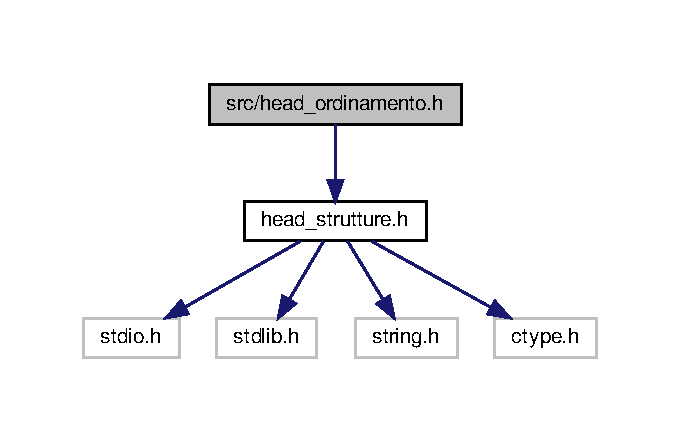
\includegraphics[width=327pt]{head__ordinamento_8h__incl}
\end{center}
\end{figure}
This graph shows which files directly or indirectly include this file\+:
\nopagebreak
\begin{figure}[H]
\begin{center}
\leavevmode
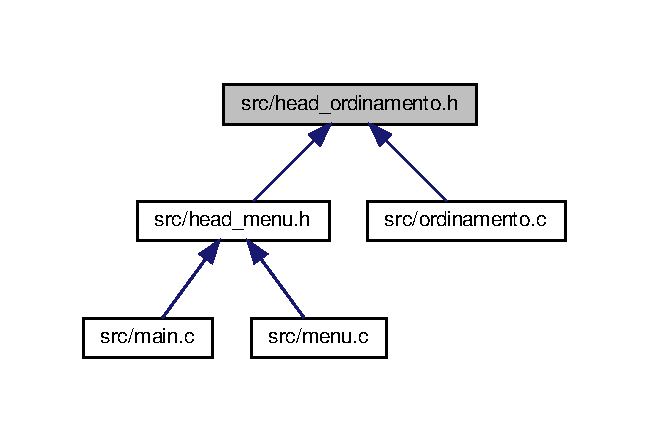
\includegraphics[width=312pt]{head__ordinamento_8h__dep__incl}
\end{center}
\end{figure}
\subsection*{Functions}
\begin{DoxyCompactItemize}
\item 
void \hyperlink{head__ordinamento_8h_a18de588a8118a4cbda403d11b1dbaf16}{print\+\_\+file} (\hyperlink{head__strutture_8h_ad83512da590021d7b336c3cb314dc228}{tipofile\+\_\+t} tipo, \hyperlink{head__strutture_8h_a3da5d27de6c586fecb3c1412cc6f1265}{campo\+\_\+record\+\_\+t} campo)
\begin{DoxyCompactList}\small\item\em Stampa l\textquotesingle{}intero file selezionato datl tipo file passato come parametro, ordinato a seconda del campo passato come parametro. \end{DoxyCompactList}\end{DoxyCompactItemize}


\subsection{Detailed Description}
Contiene le definizioni dei metodi che potrebbero essere usati da altri file. In particolare sono presenti i metodi per la visualizzazione ordinata dei record nei file. 

\subsection{Function Documentation}
\mbox{\Hypertarget{head__ordinamento_8h_a18de588a8118a4cbda403d11b1dbaf16}\label{head__ordinamento_8h_a18de588a8118a4cbda403d11b1dbaf16}} 
\index{head\+\_\+ordinamento.\+h@{head\+\_\+ordinamento.\+h}!print\+\_\+file@{print\+\_\+file}}
\index{print\+\_\+file@{print\+\_\+file}!head\+\_\+ordinamento.\+h@{head\+\_\+ordinamento.\+h}}
\subsubsection{\texorpdfstring{print\+\_\+file()}{print\_file()}}
{\footnotesize\ttfamily void print\+\_\+file (\begin{DoxyParamCaption}\item[{\hyperlink{head__strutture_8h_ad83512da590021d7b336c3cb314dc228}{tipofile\+\_\+t}}]{tipo,  }\item[{\hyperlink{head__strutture_8h_a3da5d27de6c586fecb3c1412cc6f1265}{campo\+\_\+record\+\_\+t}}]{campo }\end{DoxyParamCaption})}



Stampa l\textquotesingle{}intero file selezionato datl tipo file passato come parametro, ordinato a seconda del campo passato come parametro. 


\begin{DoxyParams}{Parameters}
{\em tipofile\+\_\+t} & tipo \\
\hline
{\em campo\+\_\+record\+\_\+t} & campo \\
\hline
\end{DoxyParams}

\hypertarget{head__strutture_8h}{}\section{src/head\+\_\+strutture.h File Reference}
\label{head__strutture_8h}\index{src/head\+\_\+strutture.\+h@{src/head\+\_\+strutture.\+h}}
{\ttfamily \#include $<$stdio.\+h$>$}\newline
{\ttfamily \#include $<$stdlib.\+h$>$}\newline
{\ttfamily \#include $<$string.\+h$>$}\newline
{\ttfamily \#include $<$ctype.\+h$>$}\newline
Include dependency graph for head\+\_\+strutture.\+h\+:
\nopagebreak
\begin{figure}[H]
\begin{center}
\leavevmode
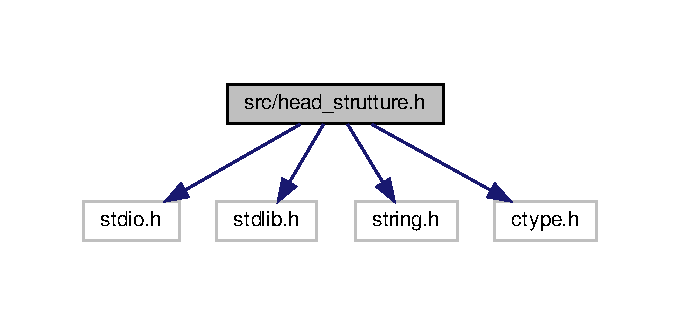
\includegraphics[width=327pt]{head__strutture_8h__incl}
\end{center}
\end{figure}
This graph shows which files directly or indirectly include this file\+:
\nopagebreak
\begin{figure}[H]
\begin{center}
\leavevmode
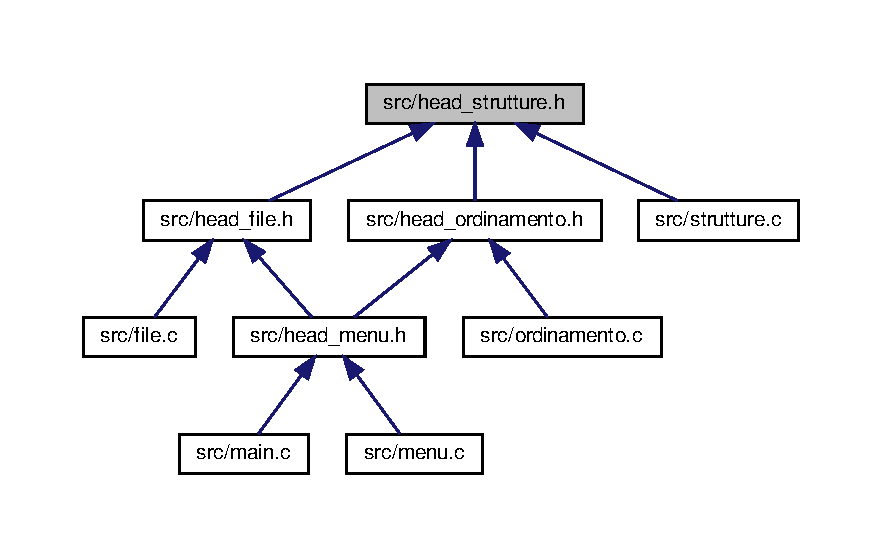
\includegraphics[width=350pt]{head__strutture_8h__dep__incl}
\end{center}
\end{figure}
\subsection*{Data Structures}
\begin{DoxyCompactItemize}
\item 
struct \hyperlink{structprodotto}{prodotto}
\begin{DoxyCompactList}\small\item\em Struttura dati Prodotto. \end{DoxyCompactList}\item 
struct \hyperlink{structpersona}{persona}
\begin{DoxyCompactList}\small\item\em Struttura dati Persona. \end{DoxyCompactList}\item 
struct \hyperlink{structsessione}{sessione}
\begin{DoxyCompactList}\small\item\em Struttura dati Sessione. \end{DoxyCompactList}\item 
struct \hyperlink{structtree__node}{tree\+\_\+node}
\begin{DoxyCompactList}\small\item\em Struttura dati tree\+\_\+noode.~\newline
Definisce un nodo di un albero binario.~\newline
Puo\textquotesingle{} essere usato sia per le strutture prodotti che per quelle persona, per questo e\textquotesingle{} presente un componente per ciascuno. \end{DoxyCompactList}\end{DoxyCompactItemize}
\subsection*{Macros}
\begin{DoxyCompactItemize}
\item 
\#define \hyperlink{head__strutture_8h_acdbdd133f0d7b6204e88098f8fb431da}{D\+E\+F\+I\+N\+I\+Z\+I\+O\+NI}
\item 
\#define \hyperlink{head__strutture_8h_adb31c7df85b5ee0c0604304f7dacea5b}{N\+O\+V\+I\+T\+A\+\_\+\+L\+E\+N\+G\+TH}~401
\item 
\#define \hyperlink{head__strutture_8h_a4062b22785fbd1c2eeb0d4b227511c18}{P\+E\+R\+S\+O\+N\+E\+\_\+\+L\+E\+N\+G\+TH}~20
\item 
\#define \hyperlink{head__strutture_8h_a07c12b5e330257e579730be4cb1183f3}{P\+R\+O\+D\+O\+T\+T\+I\+\_\+\+L\+E\+N\+G\+TH}~40
\item 
\#define \hyperlink{head__strutture_8h_a02a2d760654535b960eb191cc7d10bd7}{I\+D\+\_\+\+P\+E\+R\+S\+O\+N\+E\+\_\+\+L\+E\+N\+G\+TH}~5
\item 
\#define \hyperlink{head__strutture_8h_adf3e9636b5c21628547f626ff5ed9900}{I\+D\+\_\+\+P\+R\+O\+D\+O\+T\+T\+I\+\_\+\+L\+E\+N\+G\+TH}~10
\item 
\#define \hyperlink{head__strutture_8h_a7ffe50908e1b466b1f5dc694bf22b4c9}{N\+O\+M\+E\+\_\+\+D\+E\+F\+A\+U\+LT}~\char`\"{}default\char`\"{}
\item 
\#define \hyperlink{head__strutture_8h_ae4e9644c3fad61b59eb511bdfa00d66e}{C\+O\+G\+N\+O\+M\+E\+\_\+\+D\+E\+F\+A\+U\+LT}~\char`\"{}default\char`\"{}
\item 
\#define \hyperlink{head__strutture_8h_ac1cef138404e8b6ca16f328a0c999a1b}{I\+D\+\_\+\+D\+E\+F\+A\+U\+LT}~1
\item 
\#define \hyperlink{head__strutture_8h_a21dcded73c8cbdff1f457fb8885037f2}{P\+S\+W\+\_\+\+D\+E\+F\+A\+U\+LT}~\char`\"{}default\char`\"{}
\item 
\#define \hyperlink{head__strutture_8h_a34834adb1037d7bdd8f31f97fd1c3b51}{D\+E\+F\+A\+U\+L\+T\+\_\+\+I\+D\+\_\+\+S\+E\+S\+S\+I\+ON}~0
\item 
\#define \hyperlink{head__strutture_8h_a10220eb5edbdde03056f5060c11c0b15}{D\+E\+F\+A\+U\+L\+T\+\_\+\+P\+S\+W\+\_\+\+S\+E\+S\+S\+I\+ON}~\char`\"{}password\char`\"{}
\item 
\#define \hyperlink{head__strutture_8h_a46acf58c198f5756a3d120e33bfc2e46}{D\+E\+F\+A\+U\+L\+T\+\_\+\+M\+E\+NU}~\hyperlink{head__strutture_8h_a905479d79c2aa8410d2fc374bc75cc5ba437577c424b4ee256943fac303178144}{nolog}
\item 
\#define \hyperlink{head__strutture_8h_a1bcf6fc7b5c5bbae56a592b0ef9d91e2}{D\+E\+F\+A\+U\+L\+T\+\_\+\+S\+C\+E\+L\+TA}~0
\item 
\#define \hyperlink{head__strutture_8h_ac8b9e41b417d106b76d0f66d9edd1559}{E\+N\+U\+M\+E\+R\+A\+T\+O\+RI}
\item 
\#define \hyperlink{head__strutture_8h_ab96fd9044fe06617b2cf818b78e2a50e}{S\+T\+R\+U\+T\+T\+U\+RE}
\end{DoxyCompactItemize}
\subsection*{Typedefs}
\begin{DoxyCompactItemize}
\item 
typedef enum \hyperlink{head__strutture_8h_a20f710d6a73f95164e79b59ee0b883c2}{campo\+\_\+record} \hyperlink{head__strutture_8h_a3da5d27de6c586fecb3c1412cc6f1265}{campo\+\_\+record\+\_\+t}
\begin{DoxyCompactList}\small\item\em Indica il campo scelto nella selezione di ordinamento. \end{DoxyCompactList}\item 
typedef enum \hyperlink{head__strutture_8h_a905479d79c2aa8410d2fc374bc75cc5b}{menu} \hyperlink{head__strutture_8h_a27938a0a874a833cfee26456c5d730b1}{menu\+\_\+t}
\begin{DoxyCompactList}\small\item\em Indica il tipo di menu\textquotesingle{} che deve essere visualizzato. \end{DoxyCompactList}\item 
typedef enum \hyperlink{head__strutture_8h_a7685164e8daeb6c2998e408a80d9ea05}{tipofile} \hyperlink{head__strutture_8h_ad83512da590021d7b336c3cb314dc228}{tipofile\+\_\+t}
\begin{DoxyCompactList}\small\item\em Indica il file da usare. \end{DoxyCompactList}\item 
typedef struct \hyperlink{structprodotto}{prodotto} \hyperlink{head__strutture_8h_afec16ee1fceb6c05f4be3538f36b1997}{prodotto\+\_\+t}
\begin{DoxyCompactList}\small\item\em Struttura dati Prodotto. \end{DoxyCompactList}\item 
typedef struct \hyperlink{structpersona}{persona} \hyperlink{head__strutture_8h_a58439881922e3f6e7ed51e352f2a0c1c}{persona\+\_\+t}
\begin{DoxyCompactList}\small\item\em Struttura dati Persona. \end{DoxyCompactList}\item 
typedef struct \hyperlink{structsessione}{sessione} \hyperlink{head__strutture_8h_a784ca7b7fa64cbb661eb0c903348c1ce}{sessione\+\_\+t}
\begin{DoxyCompactList}\small\item\em Struttura dati Sessione. \end{DoxyCompactList}\item 
typedef struct \hyperlink{structtree__node}{tree\+\_\+node} \hyperlink{head__strutture_8h_a4ef1b6d5b50a013be973ef01962dc932}{tree\+\_\+node\+\_\+t}
\begin{DoxyCompactList}\small\item\em Struttura dati tree\+\_\+noode.~\newline
Definisce un nodo di un albero binario.~\newline
Puo\textquotesingle{} essere usato sia per le strutture prodotti che per quelle persona, per questo e\textquotesingle{} presente un componente per ciascuno. \end{DoxyCompactList}\end{DoxyCompactItemize}
\subsection*{Enumerations}
\begin{DoxyCompactItemize}
\item 
enum \hyperlink{head__strutture_8h_a20f710d6a73f95164e79b59ee0b883c2}{campo\+\_\+record} \{ \newline
\hyperlink{head__strutture_8h_a20f710d6a73f95164e79b59ee0b883c2acc4d0ac26924c7ec496b4805bdce5444}{nome}, 
\hyperlink{head__strutture_8h_a20f710d6a73f95164e79b59ee0b883c2a80c5c59ca7d13a4954c27d4f9972d431}{cognome}, 
\hyperlink{head__strutture_8h_a20f710d6a73f95164e79b59ee0b883c2a280d7329079c73a4a5df3f35697b60b1}{id}, 
\hyperlink{head__strutture_8h_a20f710d6a73f95164e79b59ee0b883c2aea4067ceb66474a1327144e0fda3de76}{alfabetico}, 
\newline
\hyperlink{head__strutture_8h_a20f710d6a73f95164e79b59ee0b883c2a358fe02920fdff94e70e8d7d18e2f7d5}{prezzo}
 \}\begin{DoxyCompactList}\small\item\em Indica il campo scelto nella selezione di ordinamento. \end{DoxyCompactList}
\item 
enum \hyperlink{head__strutture_8h_a905479d79c2aa8410d2fc374bc75cc5b}{menu} \{ \newline
\hyperlink{head__strutture_8h_a905479d79c2aa8410d2fc374bc75cc5ba437577c424b4ee256943fac303178144}{nolog}, 
\hyperlink{head__strutture_8h_a905479d79c2aa8410d2fc374bc75cc5baaac8d4ee23e2d305f0b0a575cda066f3}{log}, 
\hyperlink{head__strutture_8h_a905479d79c2aa8410d2fc374bc75cc5ba4b7a71d241e4df8affb579af19cc162a}{novita}, 
\hyperlink{head__strutture_8h_a905479d79c2aa8410d2fc374bc75cc5ba5af3458aa4329a4359519e5057d1c91a}{prodotti}, 
\newline
\hyperlink{head__strutture_8h_a905479d79c2aa8410d2fc374bc75cc5ba3e2eb8b6a1fc0e7e62eefcabd7829e90}{clienti}, 
\hyperlink{head__strutture_8h_a905479d79c2aa8410d2fc374bc75cc5bad52548f382e3e0c4a3f3fd83fc8cb99d}{dipendenti}, 
\hyperlink{head__strutture_8h_a905479d79c2aa8410d2fc374bc75cc5ba3671359f0dc7811af63e725834dc8137}{ordinamentoP}, 
\hyperlink{head__strutture_8h_a905479d79c2aa8410d2fc374bc75cc5ba31b9a9fb36611f86c2f20a32c5dda7a7}{ordinamentoC}, 
\newline
\hyperlink{head__strutture_8h_a905479d79c2aa8410d2fc374bc75cc5baca37cab8ed1f4e68b81d33133a3fd0e2}{ordinamentoD}
 \}\begin{DoxyCompactList}\small\item\em Indica il tipo di menu\textquotesingle{} che deve essere visualizzato. \end{DoxyCompactList}
\item 
enum \hyperlink{head__strutture_8h_a7685164e8daeb6c2998e408a80d9ea05}{tipofile} \{ \hyperlink{head__strutture_8h_a7685164e8daeb6c2998e408a80d9ea05a92b14cce3e165acfbfe29c53d46c5ee1}{prod}, 
\hyperlink{head__strutture_8h_a7685164e8daeb6c2998e408a80d9ea05a0ce60226ab327f0febfe23863e3160e1}{clie}, 
\hyperlink{head__strutture_8h_a7685164e8daeb6c2998e408a80d9ea05ac812e56c599a31d53e2b3dc32494d7ec}{dipe}
 \}\begin{DoxyCompactList}\small\item\em Indica il file da usare. \end{DoxyCompactList}
\end{DoxyCompactItemize}
\subsection*{Functions}
\begin{DoxyCompactItemize}
\item 
void \hyperlink{head__strutture_8h_af2763b0dcb4f38febe8620bb4f65736d}{initialize\+\_\+session} (\hyperlink{head__strutture_8h_a784ca7b7fa64cbb661eb0c903348c1ce}{sessione\+\_\+t} $\ast$se)
\begin{DoxyCompactList}\small\item\em Inizializza le componenti di una struttura sessione. \end{DoxyCompactList}\item 
void \hyperlink{head__strutture_8h_ae517940db604a664f340a08b4c1b1ee3}{initialize\+\_\+prodotto} (\hyperlink{head__strutture_8h_afec16ee1fceb6c05f4be3538f36b1997}{prodotto\+\_\+t} $\ast$p)
\begin{DoxyCompactList}\small\item\em Inizializza le componenti di una struttura prodotto. \end{DoxyCompactList}\item 
void \hyperlink{head__strutture_8h_a973195d321eed8af362eac78b711fd0f}{initialize\+\_\+persona} (\hyperlink{head__strutture_8h_a58439881922e3f6e7ed51e352f2a0c1c}{persona\+\_\+t} $\ast$p)
\begin{DoxyCompactList}\small\item\em Inizializza le componenti di una struttura persona. \end{DoxyCompactList}\item 
void \hyperlink{head__strutture_8h_ad95b3b50d33dc0d99ce72e61aefe65e6}{get\+\_\+string} (char $\ast$stringa, int lunghezza)
\begin{DoxyCompactList}\small\item\em Estrae da stdin una stringa di lunghezza massima data e la mette nella stringa passata come parametro, pone sempre \textbackslash{}0 alla fine. \end{DoxyCompactList}\item 
void \hyperlink{head__strutture_8h_ac85ae6df551b530c1638d7ebc48ab48a}{get\+\_\+string\+\_\+file} (char $\ast$stringa, int lunghezza, F\+I\+LE $\ast$fp)
\begin{DoxyCompactList}\small\item\em Estrae dal file passato come parametro una stringa di lunghezza massima data e la mette nella stringa passata come parametro, pone sempre \textbackslash{}0 alla fine. \end{DoxyCompactList}\item 
void \hyperlink{head__strutture_8h_a4717013d0abaa8c175dafda3925c3931}{get\+\_\+persona} (\hyperlink{head__strutture_8h_a58439881922e3f6e7ed51e352f2a0c1c}{persona\+\_\+t} $\ast$\hyperlink{structpersona}{persona}, F\+I\+LE $\ast$fp)
\begin{DoxyCompactList}\small\item\em Carica in persona i dati di una riga del file clienti.\+txt o dipendenti.\+txt. \end{DoxyCompactList}\item 
void \hyperlink{head__strutture_8h_a8f08cdbfd563b68a75bef38e80c16cbc}{get\+\_\+prodotto} (\hyperlink{head__strutture_8h_afec16ee1fceb6c05f4be3538f36b1997}{prodotto\+\_\+t} $\ast$\hyperlink{structprodotto}{prodotto}, F\+I\+LE $\ast$fp)
\begin{DoxyCompactList}\small\item\em Carica in prodotto i dati di una riga del file prodotti.\+txt. \end{DoxyCompactList}\item 
int \hyperlink{head__strutture_8h_ac472caf5ab5d1500de32eb9389419a0d}{is\+\_\+unum} (char $\ast$stringa)
\begin{DoxyCompactList}\small\item\em Controlla se la stringa passata come parametro contiene solo caratteri numerici interi senza segno. \end{DoxyCompactList}\item 
int \hyperlink{head__strutture_8h_a80d803c9093f8a72403d83adbaee7c42}{is\+\_\+num} (char $\ast$stringa)
\begin{DoxyCompactList}\small\item\em Controlla se la stringa passata come parametro contiene solo caratteri numerici interi con segno. \end{DoxyCompactList}\item 
int \hyperlink{head__strutture_8h_ad112c9780a37fb8cd6c53e0475fbdc3c}{is\+\_\+ufnum} (char $\ast$stringa)
\begin{DoxyCompactList}\small\item\em Controlla se la stringa passata come parametro contiene solo caratteri numerici interi o non senza segno. \end{DoxyCompactList}\end{DoxyCompactItemize}


\subsection{Detailed Description}
Contiene le definizioni dei metodi, le strutture, gli enumeratori che potrebbero essere usati da altri file.~\newline
In particolare sono presenti i metodi per inizzializzare tipi struttura, metodi di controllo di consistenza, metodi per recuperare record dai vari file. 

\subsection{Macro Definition Documentation}
\mbox{\Hypertarget{head__strutture_8h_ae4e9644c3fad61b59eb511bdfa00d66e}\label{head__strutture_8h_ae4e9644c3fad61b59eb511bdfa00d66e}} 
\index{head\+\_\+strutture.\+h@{head\+\_\+strutture.\+h}!C\+O\+G\+N\+O\+M\+E\+\_\+\+D\+E\+F\+A\+U\+LT@{C\+O\+G\+N\+O\+M\+E\+\_\+\+D\+E\+F\+A\+U\+LT}}
\index{C\+O\+G\+N\+O\+M\+E\+\_\+\+D\+E\+F\+A\+U\+LT@{C\+O\+G\+N\+O\+M\+E\+\_\+\+D\+E\+F\+A\+U\+LT}!head\+\_\+strutture.\+h@{head\+\_\+strutture.\+h}}
\subsubsection{\texorpdfstring{C\+O\+G\+N\+O\+M\+E\+\_\+\+D\+E\+F\+A\+U\+LT}{COGNOME\_DEFAULT}}
{\footnotesize\ttfamily \#define C\+O\+G\+N\+O\+M\+E\+\_\+\+D\+E\+F\+A\+U\+LT~\char`\"{}default\char`\"{}}

\mbox{\Hypertarget{head__strutture_8h_a34834adb1037d7bdd8f31f97fd1c3b51}\label{head__strutture_8h_a34834adb1037d7bdd8f31f97fd1c3b51}} 
\index{head\+\_\+strutture.\+h@{head\+\_\+strutture.\+h}!D\+E\+F\+A\+U\+L\+T\+\_\+\+I\+D\+\_\+\+S\+E\+S\+S\+I\+ON@{D\+E\+F\+A\+U\+L\+T\+\_\+\+I\+D\+\_\+\+S\+E\+S\+S\+I\+ON}}
\index{D\+E\+F\+A\+U\+L\+T\+\_\+\+I\+D\+\_\+\+S\+E\+S\+S\+I\+ON@{D\+E\+F\+A\+U\+L\+T\+\_\+\+I\+D\+\_\+\+S\+E\+S\+S\+I\+ON}!head\+\_\+strutture.\+h@{head\+\_\+strutture.\+h}}
\subsubsection{\texorpdfstring{D\+E\+F\+A\+U\+L\+T\+\_\+\+I\+D\+\_\+\+S\+E\+S\+S\+I\+ON}{DEFAULT\_ID\_SESSION}}
{\footnotesize\ttfamily \#define D\+E\+F\+A\+U\+L\+T\+\_\+\+I\+D\+\_\+\+S\+E\+S\+S\+I\+ON~0}

\mbox{\Hypertarget{head__strutture_8h_a46acf58c198f5756a3d120e33bfc2e46}\label{head__strutture_8h_a46acf58c198f5756a3d120e33bfc2e46}} 
\index{head\+\_\+strutture.\+h@{head\+\_\+strutture.\+h}!D\+E\+F\+A\+U\+L\+T\+\_\+\+M\+E\+NU@{D\+E\+F\+A\+U\+L\+T\+\_\+\+M\+E\+NU}}
\index{D\+E\+F\+A\+U\+L\+T\+\_\+\+M\+E\+NU@{D\+E\+F\+A\+U\+L\+T\+\_\+\+M\+E\+NU}!head\+\_\+strutture.\+h@{head\+\_\+strutture.\+h}}
\subsubsection{\texorpdfstring{D\+E\+F\+A\+U\+L\+T\+\_\+\+M\+E\+NU}{DEFAULT\_MENU}}
{\footnotesize\ttfamily \#define D\+E\+F\+A\+U\+L\+T\+\_\+\+M\+E\+NU~\hyperlink{head__strutture_8h_a905479d79c2aa8410d2fc374bc75cc5ba437577c424b4ee256943fac303178144}{nolog}}

\mbox{\Hypertarget{head__strutture_8h_a10220eb5edbdde03056f5060c11c0b15}\label{head__strutture_8h_a10220eb5edbdde03056f5060c11c0b15}} 
\index{head\+\_\+strutture.\+h@{head\+\_\+strutture.\+h}!D\+E\+F\+A\+U\+L\+T\+\_\+\+P\+S\+W\+\_\+\+S\+E\+S\+S\+I\+ON@{D\+E\+F\+A\+U\+L\+T\+\_\+\+P\+S\+W\+\_\+\+S\+E\+S\+S\+I\+ON}}
\index{D\+E\+F\+A\+U\+L\+T\+\_\+\+P\+S\+W\+\_\+\+S\+E\+S\+S\+I\+ON@{D\+E\+F\+A\+U\+L\+T\+\_\+\+P\+S\+W\+\_\+\+S\+E\+S\+S\+I\+ON}!head\+\_\+strutture.\+h@{head\+\_\+strutture.\+h}}
\subsubsection{\texorpdfstring{D\+E\+F\+A\+U\+L\+T\+\_\+\+P\+S\+W\+\_\+\+S\+E\+S\+S\+I\+ON}{DEFAULT\_PSW\_SESSION}}
{\footnotesize\ttfamily \#define D\+E\+F\+A\+U\+L\+T\+\_\+\+P\+S\+W\+\_\+\+S\+E\+S\+S\+I\+ON~\char`\"{}password\char`\"{}}

\mbox{\Hypertarget{head__strutture_8h_a1bcf6fc7b5c5bbae56a592b0ef9d91e2}\label{head__strutture_8h_a1bcf6fc7b5c5bbae56a592b0ef9d91e2}} 
\index{head\+\_\+strutture.\+h@{head\+\_\+strutture.\+h}!D\+E\+F\+A\+U\+L\+T\+\_\+\+S\+C\+E\+L\+TA@{D\+E\+F\+A\+U\+L\+T\+\_\+\+S\+C\+E\+L\+TA}}
\index{D\+E\+F\+A\+U\+L\+T\+\_\+\+S\+C\+E\+L\+TA@{D\+E\+F\+A\+U\+L\+T\+\_\+\+S\+C\+E\+L\+TA}!head\+\_\+strutture.\+h@{head\+\_\+strutture.\+h}}
\subsubsection{\texorpdfstring{D\+E\+F\+A\+U\+L\+T\+\_\+\+S\+C\+E\+L\+TA}{DEFAULT\_SCELTA}}
{\footnotesize\ttfamily \#define D\+E\+F\+A\+U\+L\+T\+\_\+\+S\+C\+E\+L\+TA~0}

\mbox{\Hypertarget{head__strutture_8h_acdbdd133f0d7b6204e88098f8fb431da}\label{head__strutture_8h_acdbdd133f0d7b6204e88098f8fb431da}} 
\index{head\+\_\+strutture.\+h@{head\+\_\+strutture.\+h}!D\+E\+F\+I\+N\+I\+Z\+I\+O\+NI@{D\+E\+F\+I\+N\+I\+Z\+I\+O\+NI}}
\index{D\+E\+F\+I\+N\+I\+Z\+I\+O\+NI@{D\+E\+F\+I\+N\+I\+Z\+I\+O\+NI}!head\+\_\+strutture.\+h@{head\+\_\+strutture.\+h}}
\subsubsection{\texorpdfstring{D\+E\+F\+I\+N\+I\+Z\+I\+O\+NI}{DEFINIZIONI}}
{\footnotesize\ttfamily \#define D\+E\+F\+I\+N\+I\+Z\+I\+O\+NI}

Blocco contenente le definizioni di tutte le macro. \mbox{\Hypertarget{head__strutture_8h_ac8b9e41b417d106b76d0f66d9edd1559}\label{head__strutture_8h_ac8b9e41b417d106b76d0f66d9edd1559}} 
\index{head\+\_\+strutture.\+h@{head\+\_\+strutture.\+h}!E\+N\+U\+M\+E\+R\+A\+T\+O\+RI@{E\+N\+U\+M\+E\+R\+A\+T\+O\+RI}}
\index{E\+N\+U\+M\+E\+R\+A\+T\+O\+RI@{E\+N\+U\+M\+E\+R\+A\+T\+O\+RI}!head\+\_\+strutture.\+h@{head\+\_\+strutture.\+h}}
\subsubsection{\texorpdfstring{E\+N\+U\+M\+E\+R\+A\+T\+O\+RI}{ENUMERATORI}}
{\footnotesize\ttfamily \#define E\+N\+U\+M\+E\+R\+A\+T\+O\+RI}

Blocco contenente le definizioni di tutti gli enumeratori. \mbox{\Hypertarget{head__strutture_8h_ac1cef138404e8b6ca16f328a0c999a1b}\label{head__strutture_8h_ac1cef138404e8b6ca16f328a0c999a1b}} 
\index{head\+\_\+strutture.\+h@{head\+\_\+strutture.\+h}!I\+D\+\_\+\+D\+E\+F\+A\+U\+LT@{I\+D\+\_\+\+D\+E\+F\+A\+U\+LT}}
\index{I\+D\+\_\+\+D\+E\+F\+A\+U\+LT@{I\+D\+\_\+\+D\+E\+F\+A\+U\+LT}!head\+\_\+strutture.\+h@{head\+\_\+strutture.\+h}}
\subsubsection{\texorpdfstring{I\+D\+\_\+\+D\+E\+F\+A\+U\+LT}{ID\_DEFAULT}}
{\footnotesize\ttfamily \#define I\+D\+\_\+\+D\+E\+F\+A\+U\+LT~1}

\mbox{\Hypertarget{head__strutture_8h_a02a2d760654535b960eb191cc7d10bd7}\label{head__strutture_8h_a02a2d760654535b960eb191cc7d10bd7}} 
\index{head\+\_\+strutture.\+h@{head\+\_\+strutture.\+h}!I\+D\+\_\+\+P\+E\+R\+S\+O\+N\+E\+\_\+\+L\+E\+N\+G\+TH@{I\+D\+\_\+\+P\+E\+R\+S\+O\+N\+E\+\_\+\+L\+E\+N\+G\+TH}}
\index{I\+D\+\_\+\+P\+E\+R\+S\+O\+N\+E\+\_\+\+L\+E\+N\+G\+TH@{I\+D\+\_\+\+P\+E\+R\+S\+O\+N\+E\+\_\+\+L\+E\+N\+G\+TH}!head\+\_\+strutture.\+h@{head\+\_\+strutture.\+h}}
\subsubsection{\texorpdfstring{I\+D\+\_\+\+P\+E\+R\+S\+O\+N\+E\+\_\+\+L\+E\+N\+G\+TH}{ID\_PERSONE\_LENGTH}}
{\footnotesize\ttfamily \#define I\+D\+\_\+\+P\+E\+R\+S\+O\+N\+E\+\_\+\+L\+E\+N\+G\+TH~5}

\mbox{\Hypertarget{head__strutture_8h_adf3e9636b5c21628547f626ff5ed9900}\label{head__strutture_8h_adf3e9636b5c21628547f626ff5ed9900}} 
\index{head\+\_\+strutture.\+h@{head\+\_\+strutture.\+h}!I\+D\+\_\+\+P\+R\+O\+D\+O\+T\+T\+I\+\_\+\+L\+E\+N\+G\+TH@{I\+D\+\_\+\+P\+R\+O\+D\+O\+T\+T\+I\+\_\+\+L\+E\+N\+G\+TH}}
\index{I\+D\+\_\+\+P\+R\+O\+D\+O\+T\+T\+I\+\_\+\+L\+E\+N\+G\+TH@{I\+D\+\_\+\+P\+R\+O\+D\+O\+T\+T\+I\+\_\+\+L\+E\+N\+G\+TH}!head\+\_\+strutture.\+h@{head\+\_\+strutture.\+h}}
\subsubsection{\texorpdfstring{I\+D\+\_\+\+P\+R\+O\+D\+O\+T\+T\+I\+\_\+\+L\+E\+N\+G\+TH}{ID\_PRODOTTI\_LENGTH}}
{\footnotesize\ttfamily \#define I\+D\+\_\+\+P\+R\+O\+D\+O\+T\+T\+I\+\_\+\+L\+E\+N\+G\+TH~10}

\mbox{\Hypertarget{head__strutture_8h_a7ffe50908e1b466b1f5dc694bf22b4c9}\label{head__strutture_8h_a7ffe50908e1b466b1f5dc694bf22b4c9}} 
\index{head\+\_\+strutture.\+h@{head\+\_\+strutture.\+h}!N\+O\+M\+E\+\_\+\+D\+E\+F\+A\+U\+LT@{N\+O\+M\+E\+\_\+\+D\+E\+F\+A\+U\+LT}}
\index{N\+O\+M\+E\+\_\+\+D\+E\+F\+A\+U\+LT@{N\+O\+M\+E\+\_\+\+D\+E\+F\+A\+U\+LT}!head\+\_\+strutture.\+h@{head\+\_\+strutture.\+h}}
\subsubsection{\texorpdfstring{N\+O\+M\+E\+\_\+\+D\+E\+F\+A\+U\+LT}{NOME\_DEFAULT}}
{\footnotesize\ttfamily \#define N\+O\+M\+E\+\_\+\+D\+E\+F\+A\+U\+LT~\char`\"{}default\char`\"{}}

\mbox{\Hypertarget{head__strutture_8h_adb31c7df85b5ee0c0604304f7dacea5b}\label{head__strutture_8h_adb31c7df85b5ee0c0604304f7dacea5b}} 
\index{head\+\_\+strutture.\+h@{head\+\_\+strutture.\+h}!N\+O\+V\+I\+T\+A\+\_\+\+L\+E\+N\+G\+TH@{N\+O\+V\+I\+T\+A\+\_\+\+L\+E\+N\+G\+TH}}
\index{N\+O\+V\+I\+T\+A\+\_\+\+L\+E\+N\+G\+TH@{N\+O\+V\+I\+T\+A\+\_\+\+L\+E\+N\+G\+TH}!head\+\_\+strutture.\+h@{head\+\_\+strutture.\+h}}
\subsubsection{\texorpdfstring{N\+O\+V\+I\+T\+A\+\_\+\+L\+E\+N\+G\+TH}{NOVITA\_LENGTH}}
{\footnotesize\ttfamily \#define N\+O\+V\+I\+T\+A\+\_\+\+L\+E\+N\+G\+TH~401}

\mbox{\Hypertarget{head__strutture_8h_a4062b22785fbd1c2eeb0d4b227511c18}\label{head__strutture_8h_a4062b22785fbd1c2eeb0d4b227511c18}} 
\index{head\+\_\+strutture.\+h@{head\+\_\+strutture.\+h}!P\+E\+R\+S\+O\+N\+E\+\_\+\+L\+E\+N\+G\+TH@{P\+E\+R\+S\+O\+N\+E\+\_\+\+L\+E\+N\+G\+TH}}
\index{P\+E\+R\+S\+O\+N\+E\+\_\+\+L\+E\+N\+G\+TH@{P\+E\+R\+S\+O\+N\+E\+\_\+\+L\+E\+N\+G\+TH}!head\+\_\+strutture.\+h@{head\+\_\+strutture.\+h}}
\subsubsection{\texorpdfstring{P\+E\+R\+S\+O\+N\+E\+\_\+\+L\+E\+N\+G\+TH}{PERSONE\_LENGTH}}
{\footnotesize\ttfamily \#define P\+E\+R\+S\+O\+N\+E\+\_\+\+L\+E\+N\+G\+TH~20}

\mbox{\Hypertarget{head__strutture_8h_a07c12b5e330257e579730be4cb1183f3}\label{head__strutture_8h_a07c12b5e330257e579730be4cb1183f3}} 
\index{head\+\_\+strutture.\+h@{head\+\_\+strutture.\+h}!P\+R\+O\+D\+O\+T\+T\+I\+\_\+\+L\+E\+N\+G\+TH@{P\+R\+O\+D\+O\+T\+T\+I\+\_\+\+L\+E\+N\+G\+TH}}
\index{P\+R\+O\+D\+O\+T\+T\+I\+\_\+\+L\+E\+N\+G\+TH@{P\+R\+O\+D\+O\+T\+T\+I\+\_\+\+L\+E\+N\+G\+TH}!head\+\_\+strutture.\+h@{head\+\_\+strutture.\+h}}
\subsubsection{\texorpdfstring{P\+R\+O\+D\+O\+T\+T\+I\+\_\+\+L\+E\+N\+G\+TH}{PRODOTTI\_LENGTH}}
{\footnotesize\ttfamily \#define P\+R\+O\+D\+O\+T\+T\+I\+\_\+\+L\+E\+N\+G\+TH~40}

\mbox{\Hypertarget{head__strutture_8h_a21dcded73c8cbdff1f457fb8885037f2}\label{head__strutture_8h_a21dcded73c8cbdff1f457fb8885037f2}} 
\index{head\+\_\+strutture.\+h@{head\+\_\+strutture.\+h}!P\+S\+W\+\_\+\+D\+E\+F\+A\+U\+LT@{P\+S\+W\+\_\+\+D\+E\+F\+A\+U\+LT}}
\index{P\+S\+W\+\_\+\+D\+E\+F\+A\+U\+LT@{P\+S\+W\+\_\+\+D\+E\+F\+A\+U\+LT}!head\+\_\+strutture.\+h@{head\+\_\+strutture.\+h}}
\subsubsection{\texorpdfstring{P\+S\+W\+\_\+\+D\+E\+F\+A\+U\+LT}{PSW\_DEFAULT}}
{\footnotesize\ttfamily \#define P\+S\+W\+\_\+\+D\+E\+F\+A\+U\+LT~\char`\"{}default\char`\"{}}

\mbox{\Hypertarget{head__strutture_8h_ab96fd9044fe06617b2cf818b78e2a50e}\label{head__strutture_8h_ab96fd9044fe06617b2cf818b78e2a50e}} 
\index{head\+\_\+strutture.\+h@{head\+\_\+strutture.\+h}!S\+T\+R\+U\+T\+T\+U\+RE@{S\+T\+R\+U\+T\+T\+U\+RE}}
\index{S\+T\+R\+U\+T\+T\+U\+RE@{S\+T\+R\+U\+T\+T\+U\+RE}!head\+\_\+strutture.\+h@{head\+\_\+strutture.\+h}}
\subsubsection{\texorpdfstring{S\+T\+R\+U\+T\+T\+U\+RE}{STRUTTURE}}
{\footnotesize\ttfamily \#define S\+T\+R\+U\+T\+T\+U\+RE}

Blocco contenente le definizioni di tutte le strutture. 

\subsection{Typedef Documentation}
\mbox{\Hypertarget{head__strutture_8h_a3da5d27de6c586fecb3c1412cc6f1265}\label{head__strutture_8h_a3da5d27de6c586fecb3c1412cc6f1265}} 
\index{head\+\_\+strutture.\+h@{head\+\_\+strutture.\+h}!campo\+\_\+record\+\_\+t@{campo\+\_\+record\+\_\+t}}
\index{campo\+\_\+record\+\_\+t@{campo\+\_\+record\+\_\+t}!head\+\_\+strutture.\+h@{head\+\_\+strutture.\+h}}
\subsubsection{\texorpdfstring{campo\+\_\+record\+\_\+t}{campo\_record\_t}}
{\footnotesize\ttfamily typedef enum \hyperlink{head__strutture_8h_a20f710d6a73f95164e79b59ee0b883c2}{campo\+\_\+record}  \hyperlink{head__strutture_8h_a3da5d27de6c586fecb3c1412cc6f1265}{campo\+\_\+record\+\_\+t}}



Indica il campo scelto nella selezione di ordinamento. 

\mbox{\Hypertarget{head__strutture_8h_a27938a0a874a833cfee26456c5d730b1}\label{head__strutture_8h_a27938a0a874a833cfee26456c5d730b1}} 
\index{head\+\_\+strutture.\+h@{head\+\_\+strutture.\+h}!menu\+\_\+t@{menu\+\_\+t}}
\index{menu\+\_\+t@{menu\+\_\+t}!head\+\_\+strutture.\+h@{head\+\_\+strutture.\+h}}
\subsubsection{\texorpdfstring{menu\+\_\+t}{menu\_t}}
{\footnotesize\ttfamily typedef enum \hyperlink{head__strutture_8h_a905479d79c2aa8410d2fc374bc75cc5b}{menu}  \hyperlink{head__strutture_8h_a27938a0a874a833cfee26456c5d730b1}{menu\+\_\+t}}



Indica il tipo di menu\textquotesingle{} che deve essere visualizzato. 

\mbox{\Hypertarget{head__strutture_8h_a58439881922e3f6e7ed51e352f2a0c1c}\label{head__strutture_8h_a58439881922e3f6e7ed51e352f2a0c1c}} 
\index{head\+\_\+strutture.\+h@{head\+\_\+strutture.\+h}!persona\+\_\+t@{persona\+\_\+t}}
\index{persona\+\_\+t@{persona\+\_\+t}!head\+\_\+strutture.\+h@{head\+\_\+strutture.\+h}}
\subsubsection{\texorpdfstring{persona\+\_\+t}{persona\_t}}
{\footnotesize\ttfamily typedef struct \hyperlink{structpersona}{persona} \hyperlink{head__strutture_8h_a58439881922e3f6e7ed51e352f2a0c1c}{persona\+\_\+t}}



Struttura dati Persona. 

\mbox{\Hypertarget{head__strutture_8h_afec16ee1fceb6c05f4be3538f36b1997}\label{head__strutture_8h_afec16ee1fceb6c05f4be3538f36b1997}} 
\index{head\+\_\+strutture.\+h@{head\+\_\+strutture.\+h}!prodotto\+\_\+t@{prodotto\+\_\+t}}
\index{prodotto\+\_\+t@{prodotto\+\_\+t}!head\+\_\+strutture.\+h@{head\+\_\+strutture.\+h}}
\subsubsection{\texorpdfstring{prodotto\+\_\+t}{prodotto\_t}}
{\footnotesize\ttfamily typedef struct \hyperlink{structprodotto}{prodotto}  \hyperlink{head__strutture_8h_afec16ee1fceb6c05f4be3538f36b1997}{prodotto\+\_\+t}}



Struttura dati Prodotto. 

\mbox{\Hypertarget{head__strutture_8h_a784ca7b7fa64cbb661eb0c903348c1ce}\label{head__strutture_8h_a784ca7b7fa64cbb661eb0c903348c1ce}} 
\index{head\+\_\+strutture.\+h@{head\+\_\+strutture.\+h}!sessione\+\_\+t@{sessione\+\_\+t}}
\index{sessione\+\_\+t@{sessione\+\_\+t}!head\+\_\+strutture.\+h@{head\+\_\+strutture.\+h}}
\subsubsection{\texorpdfstring{sessione\+\_\+t}{sessione\_t}}
{\footnotesize\ttfamily typedef struct \hyperlink{structsessione}{sessione} \hyperlink{head__strutture_8h_a784ca7b7fa64cbb661eb0c903348c1ce}{sessione\+\_\+t}}



Struttura dati Sessione. 

\mbox{\Hypertarget{head__strutture_8h_ad83512da590021d7b336c3cb314dc228}\label{head__strutture_8h_ad83512da590021d7b336c3cb314dc228}} 
\index{head\+\_\+strutture.\+h@{head\+\_\+strutture.\+h}!tipofile\+\_\+t@{tipofile\+\_\+t}}
\index{tipofile\+\_\+t@{tipofile\+\_\+t}!head\+\_\+strutture.\+h@{head\+\_\+strutture.\+h}}
\subsubsection{\texorpdfstring{tipofile\+\_\+t}{tipofile\_t}}
{\footnotesize\ttfamily typedef enum \hyperlink{head__strutture_8h_a7685164e8daeb6c2998e408a80d9ea05}{tipofile}  \hyperlink{head__strutture_8h_ad83512da590021d7b336c3cb314dc228}{tipofile\+\_\+t}}



Indica il file da usare. 

\mbox{\Hypertarget{head__strutture_8h_a4ef1b6d5b50a013be973ef01962dc932}\label{head__strutture_8h_a4ef1b6d5b50a013be973ef01962dc932}} 
\index{head\+\_\+strutture.\+h@{head\+\_\+strutture.\+h}!tree\+\_\+node\+\_\+t@{tree\+\_\+node\+\_\+t}}
\index{tree\+\_\+node\+\_\+t@{tree\+\_\+node\+\_\+t}!head\+\_\+strutture.\+h@{head\+\_\+strutture.\+h}}
\subsubsection{\texorpdfstring{tree\+\_\+node\+\_\+t}{tree\_node\_t}}
{\footnotesize\ttfamily typedef struct \hyperlink{structtree__node}{tree\+\_\+node}  \hyperlink{head__strutture_8h_a4ef1b6d5b50a013be973ef01962dc932}{tree\+\_\+node\+\_\+t}}



Struttura dati tree\+\_\+noode.~\newline
Definisce un nodo di un albero binario.~\newline
Puo\textquotesingle{} essere usato sia per le strutture prodotti che per quelle persona, per questo e\textquotesingle{} presente un componente per ciascuno. 



\subsection{Enumeration Type Documentation}
\mbox{\Hypertarget{head__strutture_8h_a20f710d6a73f95164e79b59ee0b883c2}\label{head__strutture_8h_a20f710d6a73f95164e79b59ee0b883c2}} 
\index{head\+\_\+strutture.\+h@{head\+\_\+strutture.\+h}!campo\+\_\+record@{campo\+\_\+record}}
\index{campo\+\_\+record@{campo\+\_\+record}!head\+\_\+strutture.\+h@{head\+\_\+strutture.\+h}}
\subsubsection{\texorpdfstring{campo\+\_\+record}{campo\_record}}
{\footnotesize\ttfamily enum \hyperlink{head__strutture_8h_a20f710d6a73f95164e79b59ee0b883c2}{campo\+\_\+record}}



Indica il campo scelto nella selezione di ordinamento. 

\begin{DoxyEnumFields}{Enumerator}
\raisebox{\heightof{T}}[0pt][0pt]{\index{nome@{nome}!head\+\_\+strutture.\+h@{head\+\_\+strutture.\+h}}\index{head\+\_\+strutture.\+h@{head\+\_\+strutture.\+h}!nome@{nome}}}\mbox{\Hypertarget{head__strutture_8h_a20f710d6a73f95164e79b59ee0b883c2acc4d0ac26924c7ec496b4805bdce5444}\label{head__strutture_8h_a20f710d6a73f95164e79b59ee0b883c2acc4d0ac26924c7ec496b4805bdce5444}} 
nome&\\
\hline

\raisebox{\heightof{T}}[0pt][0pt]{\index{cognome@{cognome}!head\+\_\+strutture.\+h@{head\+\_\+strutture.\+h}}\index{head\+\_\+strutture.\+h@{head\+\_\+strutture.\+h}!cognome@{cognome}}}\mbox{\Hypertarget{head__strutture_8h_a20f710d6a73f95164e79b59ee0b883c2a80c5c59ca7d13a4954c27d4f9972d431}\label{head__strutture_8h_a20f710d6a73f95164e79b59ee0b883c2a80c5c59ca7d13a4954c27d4f9972d431}} 
cognome&\\
\hline

\raisebox{\heightof{T}}[0pt][0pt]{\index{id@{id}!head\+\_\+strutture.\+h@{head\+\_\+strutture.\+h}}\index{head\+\_\+strutture.\+h@{head\+\_\+strutture.\+h}!id@{id}}}\mbox{\Hypertarget{head__strutture_8h_a20f710d6a73f95164e79b59ee0b883c2a280d7329079c73a4a5df3f35697b60b1}\label{head__strutture_8h_a20f710d6a73f95164e79b59ee0b883c2a280d7329079c73a4a5df3f35697b60b1}} 
id&\\
\hline

\raisebox{\heightof{T}}[0pt][0pt]{\index{alfabetico@{alfabetico}!head\+\_\+strutture.\+h@{head\+\_\+strutture.\+h}}\index{head\+\_\+strutture.\+h@{head\+\_\+strutture.\+h}!alfabetico@{alfabetico}}}\mbox{\Hypertarget{head__strutture_8h_a20f710d6a73f95164e79b59ee0b883c2aea4067ceb66474a1327144e0fda3de76}\label{head__strutture_8h_a20f710d6a73f95164e79b59ee0b883c2aea4067ceb66474a1327144e0fda3de76}} 
alfabetico&\\
\hline

\raisebox{\heightof{T}}[0pt][0pt]{\index{prezzo@{prezzo}!head\+\_\+strutture.\+h@{head\+\_\+strutture.\+h}}\index{head\+\_\+strutture.\+h@{head\+\_\+strutture.\+h}!prezzo@{prezzo}}}\mbox{\Hypertarget{head__strutture_8h_a20f710d6a73f95164e79b59ee0b883c2a358fe02920fdff94e70e8d7d18e2f7d5}\label{head__strutture_8h_a20f710d6a73f95164e79b59ee0b883c2a358fe02920fdff94e70e8d7d18e2f7d5}} 
prezzo&\\
\hline

\end{DoxyEnumFields}
\mbox{\Hypertarget{head__strutture_8h_a905479d79c2aa8410d2fc374bc75cc5b}\label{head__strutture_8h_a905479d79c2aa8410d2fc374bc75cc5b}} 
\index{head\+\_\+strutture.\+h@{head\+\_\+strutture.\+h}!menu@{menu}}
\index{menu@{menu}!head\+\_\+strutture.\+h@{head\+\_\+strutture.\+h}}
\subsubsection{\texorpdfstring{menu}{menu}}
{\footnotesize\ttfamily enum \hyperlink{head__strutture_8h_a905479d79c2aa8410d2fc374bc75cc5b}{menu}}



Indica il tipo di menu\textquotesingle{} che deve essere visualizzato. 

\begin{DoxyEnumFields}{Enumerator}
\raisebox{\heightof{T}}[0pt][0pt]{\index{nolog@{nolog}!head\+\_\+strutture.\+h@{head\+\_\+strutture.\+h}}\index{head\+\_\+strutture.\+h@{head\+\_\+strutture.\+h}!nolog@{nolog}}}\mbox{\Hypertarget{head__strutture_8h_a905479d79c2aa8410d2fc374bc75cc5ba437577c424b4ee256943fac303178144}\label{head__strutture_8h_a905479d79c2aa8410d2fc374bc75cc5ba437577c424b4ee256943fac303178144}} 
nolog&\\
\hline

\raisebox{\heightof{T}}[0pt][0pt]{\index{log@{log}!head\+\_\+strutture.\+h@{head\+\_\+strutture.\+h}}\index{head\+\_\+strutture.\+h@{head\+\_\+strutture.\+h}!log@{log}}}\mbox{\Hypertarget{head__strutture_8h_a905479d79c2aa8410d2fc374bc75cc5baaac8d4ee23e2d305f0b0a575cda066f3}\label{head__strutture_8h_a905479d79c2aa8410d2fc374bc75cc5baaac8d4ee23e2d305f0b0a575cda066f3}} 
log&\\
\hline

\raisebox{\heightof{T}}[0pt][0pt]{\index{novita@{novita}!head\+\_\+strutture.\+h@{head\+\_\+strutture.\+h}}\index{head\+\_\+strutture.\+h@{head\+\_\+strutture.\+h}!novita@{novita}}}\mbox{\Hypertarget{head__strutture_8h_a905479d79c2aa8410d2fc374bc75cc5ba4b7a71d241e4df8affb579af19cc162a}\label{head__strutture_8h_a905479d79c2aa8410d2fc374bc75cc5ba4b7a71d241e4df8affb579af19cc162a}} 
novita&\\
\hline

\raisebox{\heightof{T}}[0pt][0pt]{\index{prodotti@{prodotti}!head\+\_\+strutture.\+h@{head\+\_\+strutture.\+h}}\index{head\+\_\+strutture.\+h@{head\+\_\+strutture.\+h}!prodotti@{prodotti}}}\mbox{\Hypertarget{head__strutture_8h_a905479d79c2aa8410d2fc374bc75cc5ba5af3458aa4329a4359519e5057d1c91a}\label{head__strutture_8h_a905479d79c2aa8410d2fc374bc75cc5ba5af3458aa4329a4359519e5057d1c91a}} 
prodotti&\\
\hline

\raisebox{\heightof{T}}[0pt][0pt]{\index{clienti@{clienti}!head\+\_\+strutture.\+h@{head\+\_\+strutture.\+h}}\index{head\+\_\+strutture.\+h@{head\+\_\+strutture.\+h}!clienti@{clienti}}}\mbox{\Hypertarget{head__strutture_8h_a905479d79c2aa8410d2fc374bc75cc5ba3e2eb8b6a1fc0e7e62eefcabd7829e90}\label{head__strutture_8h_a905479d79c2aa8410d2fc374bc75cc5ba3e2eb8b6a1fc0e7e62eefcabd7829e90}} 
clienti&\\
\hline

\raisebox{\heightof{T}}[0pt][0pt]{\index{dipendenti@{dipendenti}!head\+\_\+strutture.\+h@{head\+\_\+strutture.\+h}}\index{head\+\_\+strutture.\+h@{head\+\_\+strutture.\+h}!dipendenti@{dipendenti}}}\mbox{\Hypertarget{head__strutture_8h_a905479d79c2aa8410d2fc374bc75cc5bad52548f382e3e0c4a3f3fd83fc8cb99d}\label{head__strutture_8h_a905479d79c2aa8410d2fc374bc75cc5bad52548f382e3e0c4a3f3fd83fc8cb99d}} 
dipendenti&\\
\hline

\raisebox{\heightof{T}}[0pt][0pt]{\index{ordinamentoP@{ordinamentoP}!head\+\_\+strutture.\+h@{head\+\_\+strutture.\+h}}\index{head\+\_\+strutture.\+h@{head\+\_\+strutture.\+h}!ordinamentoP@{ordinamentoP}}}\mbox{\Hypertarget{head__strutture_8h_a905479d79c2aa8410d2fc374bc75cc5ba3671359f0dc7811af63e725834dc8137}\label{head__strutture_8h_a905479d79c2aa8410d2fc374bc75cc5ba3671359f0dc7811af63e725834dc8137}} 
ordinamentoP&\\
\hline

\raisebox{\heightof{T}}[0pt][0pt]{\index{ordinamentoC@{ordinamentoC}!head\+\_\+strutture.\+h@{head\+\_\+strutture.\+h}}\index{head\+\_\+strutture.\+h@{head\+\_\+strutture.\+h}!ordinamentoC@{ordinamentoC}}}\mbox{\Hypertarget{head__strutture_8h_a905479d79c2aa8410d2fc374bc75cc5ba31b9a9fb36611f86c2f20a32c5dda7a7}\label{head__strutture_8h_a905479d79c2aa8410d2fc374bc75cc5ba31b9a9fb36611f86c2f20a32c5dda7a7}} 
ordinamentoC&\\
\hline

\raisebox{\heightof{T}}[0pt][0pt]{\index{ordinamentoD@{ordinamentoD}!head\+\_\+strutture.\+h@{head\+\_\+strutture.\+h}}\index{head\+\_\+strutture.\+h@{head\+\_\+strutture.\+h}!ordinamentoD@{ordinamentoD}}}\mbox{\Hypertarget{head__strutture_8h_a905479d79c2aa8410d2fc374bc75cc5baca37cab8ed1f4e68b81d33133a3fd0e2}\label{head__strutture_8h_a905479d79c2aa8410d2fc374bc75cc5baca37cab8ed1f4e68b81d33133a3fd0e2}} 
ordinamentoD&\\
\hline

\end{DoxyEnumFields}
\mbox{\Hypertarget{head__strutture_8h_a7685164e8daeb6c2998e408a80d9ea05}\label{head__strutture_8h_a7685164e8daeb6c2998e408a80d9ea05}} 
\index{head\+\_\+strutture.\+h@{head\+\_\+strutture.\+h}!tipofile@{tipofile}}
\index{tipofile@{tipofile}!head\+\_\+strutture.\+h@{head\+\_\+strutture.\+h}}
\subsubsection{\texorpdfstring{tipofile}{tipofile}}
{\footnotesize\ttfamily enum \hyperlink{head__strutture_8h_a7685164e8daeb6c2998e408a80d9ea05}{tipofile}}



Indica il file da usare. 

\begin{DoxyEnumFields}{Enumerator}
\raisebox{\heightof{T}}[0pt][0pt]{\index{prod@{prod}!head\+\_\+strutture.\+h@{head\+\_\+strutture.\+h}}\index{head\+\_\+strutture.\+h@{head\+\_\+strutture.\+h}!prod@{prod}}}\mbox{\Hypertarget{head__strutture_8h_a7685164e8daeb6c2998e408a80d9ea05a92b14cce3e165acfbfe29c53d46c5ee1}\label{head__strutture_8h_a7685164e8daeb6c2998e408a80d9ea05a92b14cce3e165acfbfe29c53d46c5ee1}} 
prod&\\
\hline

\raisebox{\heightof{T}}[0pt][0pt]{\index{clie@{clie}!head\+\_\+strutture.\+h@{head\+\_\+strutture.\+h}}\index{head\+\_\+strutture.\+h@{head\+\_\+strutture.\+h}!clie@{clie}}}\mbox{\Hypertarget{head__strutture_8h_a7685164e8daeb6c2998e408a80d9ea05a0ce60226ab327f0febfe23863e3160e1}\label{head__strutture_8h_a7685164e8daeb6c2998e408a80d9ea05a0ce60226ab327f0febfe23863e3160e1}} 
clie&\\
\hline

\raisebox{\heightof{T}}[0pt][0pt]{\index{dipe@{dipe}!head\+\_\+strutture.\+h@{head\+\_\+strutture.\+h}}\index{head\+\_\+strutture.\+h@{head\+\_\+strutture.\+h}!dipe@{dipe}}}\mbox{\Hypertarget{head__strutture_8h_a7685164e8daeb6c2998e408a80d9ea05ac812e56c599a31d53e2b3dc32494d7ec}\label{head__strutture_8h_a7685164e8daeb6c2998e408a80d9ea05ac812e56c599a31d53e2b3dc32494d7ec}} 
dipe&\\
\hline

\end{DoxyEnumFields}


\subsection{Function Documentation}
\mbox{\Hypertarget{head__strutture_8h_a4717013d0abaa8c175dafda3925c3931}\label{head__strutture_8h_a4717013d0abaa8c175dafda3925c3931}} 
\index{head\+\_\+strutture.\+h@{head\+\_\+strutture.\+h}!get\+\_\+persona@{get\+\_\+persona}}
\index{get\+\_\+persona@{get\+\_\+persona}!head\+\_\+strutture.\+h@{head\+\_\+strutture.\+h}}
\subsubsection{\texorpdfstring{get\+\_\+persona()}{get\_persona()}}
{\footnotesize\ttfamily void get\+\_\+persona (\begin{DoxyParamCaption}\item[{\hyperlink{head__strutture_8h_a58439881922e3f6e7ed51e352f2a0c1c}{persona\+\_\+t} $\ast$}]{persona,  }\item[{F\+I\+LE $\ast$}]{fp }\end{DoxyParamCaption})}



Carica in persona i dati di una riga del file clienti.\+txt o dipendenti.\+txt. 

Si ipotizza di essere nella posizione giusta e che il puntatore al file sia open.~\newline
Alla fine lascia il puntatore sulla nuova riga se esiste. 
\begin{DoxyParams}{Parameters}
{\em persona\+\_\+t} & $\ast$persona \\
\hline
{\em F\+I\+LE} & $\ast$file \\
\hline
\end{DoxyParams}
\mbox{\Hypertarget{head__strutture_8h_a8f08cdbfd563b68a75bef38e80c16cbc}\label{head__strutture_8h_a8f08cdbfd563b68a75bef38e80c16cbc}} 
\index{head\+\_\+strutture.\+h@{head\+\_\+strutture.\+h}!get\+\_\+prodotto@{get\+\_\+prodotto}}
\index{get\+\_\+prodotto@{get\+\_\+prodotto}!head\+\_\+strutture.\+h@{head\+\_\+strutture.\+h}}
\subsubsection{\texorpdfstring{get\+\_\+prodotto()}{get\_prodotto()}}
{\footnotesize\ttfamily void get\+\_\+prodotto (\begin{DoxyParamCaption}\item[{\hyperlink{head__strutture_8h_afec16ee1fceb6c05f4be3538f36b1997}{prodotto\+\_\+t} $\ast$}]{prodotto,  }\item[{F\+I\+LE $\ast$}]{fp }\end{DoxyParamCaption})}



Carica in prodotto i dati di una riga del file prodotti.\+txt. 

Si ipotizza di essere nella posizione giusta e che il puntatore al file sia open.~\newline
Alla fine lascia il puntatore sulla nuova riga se esiste. 
\begin{DoxyParams}{Parameters}
{\em prodotto\+\_\+t} & $\ast$prodotto \\
\hline
{\em F\+I\+LE} & $\ast$file \\
\hline
\end{DoxyParams}
\mbox{\Hypertarget{head__strutture_8h_ad95b3b50d33dc0d99ce72e61aefe65e6}\label{head__strutture_8h_ad95b3b50d33dc0d99ce72e61aefe65e6}} 
\index{head\+\_\+strutture.\+h@{head\+\_\+strutture.\+h}!get\+\_\+string@{get\+\_\+string}}
\index{get\+\_\+string@{get\+\_\+string}!head\+\_\+strutture.\+h@{head\+\_\+strutture.\+h}}
\subsubsection{\texorpdfstring{get\+\_\+string()}{get\_string()}}
{\footnotesize\ttfamily void get\+\_\+string (\begin{DoxyParamCaption}\item[{char $\ast$}]{stringa,  }\item[{int}]{lunghezza }\end{DoxyParamCaption})}



Estrae da stdin una stringa di lunghezza massima data e la mette nella stringa passata come parametro, pone sempre \textbackslash{}0 alla fine. 

Se ci sono piu\textquotesingle{} caratteri di quelli ammissibili svuota anche il buffer. 
\begin{DoxyParams}{Parameters}
{\em char} & $\ast$stringa \\
\hline
{\em int} & lunghezza \\
\hline
\end{DoxyParams}
\mbox{\Hypertarget{head__strutture_8h_ac85ae6df551b530c1638d7ebc48ab48a}\label{head__strutture_8h_ac85ae6df551b530c1638d7ebc48ab48a}} 
\index{head\+\_\+strutture.\+h@{head\+\_\+strutture.\+h}!get\+\_\+string\+\_\+file@{get\+\_\+string\+\_\+file}}
\index{get\+\_\+string\+\_\+file@{get\+\_\+string\+\_\+file}!head\+\_\+strutture.\+h@{head\+\_\+strutture.\+h}}
\subsubsection{\texorpdfstring{get\+\_\+string\+\_\+file()}{get\_string\_file()}}
{\footnotesize\ttfamily void get\+\_\+string\+\_\+file (\begin{DoxyParamCaption}\item[{char $\ast$}]{stringa,  }\item[{int}]{lunghezza,  }\item[{F\+I\+LE $\ast$}]{fp }\end{DoxyParamCaption})}



Estrae dal file passato come parametro una stringa di lunghezza massima data e la mette nella stringa passata come parametro, pone sempre \textbackslash{}0 alla fine. 

Se ci sono piu\textquotesingle{} caratteri di quelli ammissibili svuota anche il buffer. A\+T\+T\+E\+N\+Z\+I\+O\+NE\+: Questo metodo non e\textquotesingle{} mai stato utilizzato nel programma quindi potrebbe non funzionare correttamente, potrebbe tornare utile. 
\begin{DoxyParams}{Parameters}
{\em char} & $\ast$stringa \\
\hline
{\em int} & lunghezza \\
\hline
{\em F\+I\+LE} & $\ast$fp \\
\hline
\end{DoxyParams}
\mbox{\Hypertarget{head__strutture_8h_a973195d321eed8af362eac78b711fd0f}\label{head__strutture_8h_a973195d321eed8af362eac78b711fd0f}} 
\index{head\+\_\+strutture.\+h@{head\+\_\+strutture.\+h}!initialize\+\_\+persona@{initialize\+\_\+persona}}
\index{initialize\+\_\+persona@{initialize\+\_\+persona}!head\+\_\+strutture.\+h@{head\+\_\+strutture.\+h}}
\subsubsection{\texorpdfstring{initialize\+\_\+persona()}{initialize\_persona()}}
{\footnotesize\ttfamily void initialize\+\_\+persona (\begin{DoxyParamCaption}\item[{\hyperlink{head__strutture_8h_a58439881922e3f6e7ed51e352f2a0c1c}{persona\+\_\+t} $\ast$}]{p }\end{DoxyParamCaption})}



Inizializza le componenti di una struttura persona. 


\begin{DoxyParams}{Parameters}
{\em persona\+\_\+t} & $\ast$persona \\
\hline
\end{DoxyParams}
\mbox{\Hypertarget{head__strutture_8h_ae517940db604a664f340a08b4c1b1ee3}\label{head__strutture_8h_ae517940db604a664f340a08b4c1b1ee3}} 
\index{head\+\_\+strutture.\+h@{head\+\_\+strutture.\+h}!initialize\+\_\+prodotto@{initialize\+\_\+prodotto}}
\index{initialize\+\_\+prodotto@{initialize\+\_\+prodotto}!head\+\_\+strutture.\+h@{head\+\_\+strutture.\+h}}
\subsubsection{\texorpdfstring{initialize\+\_\+prodotto()}{initialize\_prodotto()}}
{\footnotesize\ttfamily void initialize\+\_\+prodotto (\begin{DoxyParamCaption}\item[{\hyperlink{head__strutture_8h_afec16ee1fceb6c05f4be3538f36b1997}{prodotto\+\_\+t} $\ast$}]{p }\end{DoxyParamCaption})}



Inizializza le componenti di una struttura prodotto. 


\begin{DoxyParams}{Parameters}
{\em prodotto\+\_\+t} & $\ast$prodotto \\
\hline
\end{DoxyParams}
\mbox{\Hypertarget{head__strutture_8h_af2763b0dcb4f38febe8620bb4f65736d}\label{head__strutture_8h_af2763b0dcb4f38febe8620bb4f65736d}} 
\index{head\+\_\+strutture.\+h@{head\+\_\+strutture.\+h}!initialize\+\_\+session@{initialize\+\_\+session}}
\index{initialize\+\_\+session@{initialize\+\_\+session}!head\+\_\+strutture.\+h@{head\+\_\+strutture.\+h}}
\subsubsection{\texorpdfstring{initialize\+\_\+session()}{initialize\_session()}}
{\footnotesize\ttfamily void initialize\+\_\+session (\begin{DoxyParamCaption}\item[{\hyperlink{head__strutture_8h_a784ca7b7fa64cbb661eb0c903348c1ce}{sessione\+\_\+t} $\ast$}]{se }\end{DoxyParamCaption})}



Inizializza le componenti di una struttura sessione. 


\begin{DoxyParams}{Parameters}
{\em sessione\+\_\+t} & $\ast$sessione \\
\hline
\end{DoxyParams}
\mbox{\Hypertarget{head__strutture_8h_a80d803c9093f8a72403d83adbaee7c42}\label{head__strutture_8h_a80d803c9093f8a72403d83adbaee7c42}} 
\index{head\+\_\+strutture.\+h@{head\+\_\+strutture.\+h}!is\+\_\+num@{is\+\_\+num}}
\index{is\+\_\+num@{is\+\_\+num}!head\+\_\+strutture.\+h@{head\+\_\+strutture.\+h}}
\subsubsection{\texorpdfstring{is\+\_\+num()}{is\_num()}}
{\footnotesize\ttfamily int is\+\_\+num (\begin{DoxyParamCaption}\item[{char $\ast$}]{stringa }\end{DoxyParamCaption})}



Controlla se la stringa passata come parametro contiene solo caratteri numerici interi con segno. 

Ritorna 0 se la stringa corrisponde al tipo definito, -\/1 altrimenti. 
\begin{DoxyParams}{Parameters}
{\em char} & $\ast$stringa \\
\hline
\end{DoxyParams}
\begin{DoxyReturn}{Returns}
int 
\end{DoxyReturn}
\mbox{\Hypertarget{head__strutture_8h_ad112c9780a37fb8cd6c53e0475fbdc3c}\label{head__strutture_8h_ad112c9780a37fb8cd6c53e0475fbdc3c}} 
\index{head\+\_\+strutture.\+h@{head\+\_\+strutture.\+h}!is\+\_\+ufnum@{is\+\_\+ufnum}}
\index{is\+\_\+ufnum@{is\+\_\+ufnum}!head\+\_\+strutture.\+h@{head\+\_\+strutture.\+h}}
\subsubsection{\texorpdfstring{is\+\_\+ufnum()}{is\_ufnum()}}
{\footnotesize\ttfamily int is\+\_\+ufnum (\begin{DoxyParamCaption}\item[{char $\ast$}]{stringa }\end{DoxyParamCaption})}



Controlla se la stringa passata come parametro contiene solo caratteri numerici interi o non senza segno. 

Ritorna 0 se la stringa corrisponde al tipo definito, -\/1 altrimenti. 
\begin{DoxyParams}{Parameters}
{\em char} & $\ast$stringa \\
\hline
\end{DoxyParams}
\begin{DoxyReturn}{Returns}
int 
\end{DoxyReturn}
\begin{DoxyRefDesc}{Bug}
\item[\hyperlink{bug__bug000002}{Bug}]E\textquotesingle{} stato necessario includere sia , che . quindi potrebbe avere un comportamento leggermente diverso se usato un delimitatore di cifre diverso da quello definito dal proprio sistema (non causa comunque errori gravi, si perde al massimo la parte decimale). \end{DoxyRefDesc}
\mbox{\Hypertarget{head__strutture_8h_ac472caf5ab5d1500de32eb9389419a0d}\label{head__strutture_8h_ac472caf5ab5d1500de32eb9389419a0d}} 
\index{head\+\_\+strutture.\+h@{head\+\_\+strutture.\+h}!is\+\_\+unum@{is\+\_\+unum}}
\index{is\+\_\+unum@{is\+\_\+unum}!head\+\_\+strutture.\+h@{head\+\_\+strutture.\+h}}
\subsubsection{\texorpdfstring{is\+\_\+unum()}{is\_unum()}}
{\footnotesize\ttfamily int is\+\_\+unum (\begin{DoxyParamCaption}\item[{char $\ast$}]{stringa }\end{DoxyParamCaption})}



Controlla se la stringa passata come parametro contiene solo caratteri numerici interi senza segno. 

Ritorna 0 se la stringa corrisponde al tipo definito, -\/1 altrimenti. 
\begin{DoxyParams}{Parameters}
{\em char} & $\ast$stringa \\
\hline
\end{DoxyParams}
\begin{DoxyReturn}{Returns}
int 
\end{DoxyReturn}

\hypertarget{main_8c}{}\section{src/main.c File Reference}
\label{main_8c}\index{src/main.\+c@{src/main.\+c}}
{\ttfamily \#include \char`\"{}head\+\_\+menu.\+h\char`\"{}}\newline
Include dependency graph for main.\+c\+:
\nopagebreak
\begin{figure}[H]
\begin{center}
\leavevmode
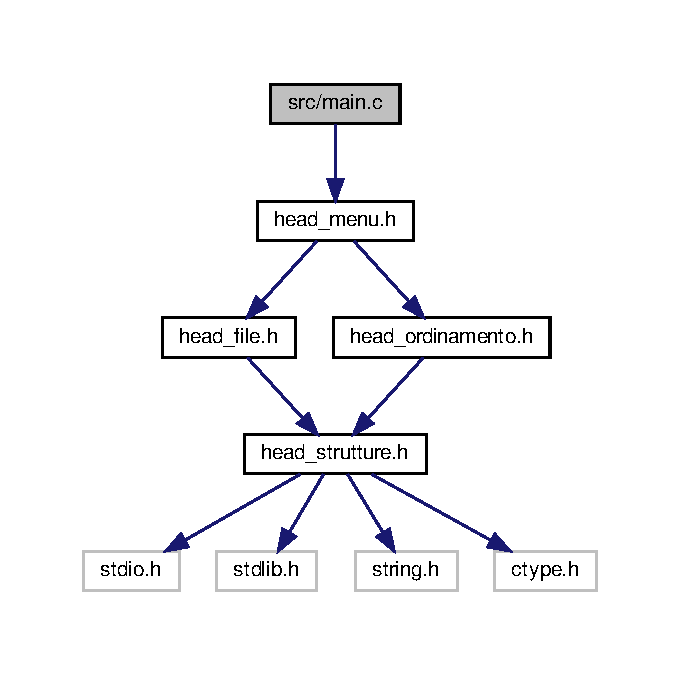
\includegraphics[width=327pt]{main_8c__incl}
\end{center}
\end{figure}
\subsection*{Functions}
\begin{DoxyCompactItemize}
\item 
int \hyperlink{main_8c_a840291bc02cba5474a4cb46a9b9566fe}{main} (void)
\end{DoxyCompactItemize}


\subsection{Detailed Description}
\begin{DoxyAuthor}{Author}
Davi\textquotesingle{} Luca
\end{DoxyAuthor}
Questo file contiene solamente il metodo main nel quale vengono richiamati i due metodi principali per la navigazione 

\subsection{Function Documentation}
\mbox{\Hypertarget{main_8c_a840291bc02cba5474a4cb46a9b9566fe}\label{main_8c_a840291bc02cba5474a4cb46a9b9566fe}} 
\index{main.\+c@{main.\+c}!main@{main}}
\index{main@{main}!main.\+c@{main.\+c}}
\subsubsection{\texorpdfstring{main()}{main()}}
{\footnotesize\ttfamily int main (\begin{DoxyParamCaption}\item[{void}]{ }\end{DoxyParamCaption})}


\hypertarget{menu_8c}{}\section{src/menu.c File Reference}
\label{menu_8c}\index{src/menu.\+c@{src/menu.\+c}}
{\ttfamily \#include \char`\"{}head\+\_\+menu.\+h\char`\"{}}\newline
Include dependency graph for menu.\+c\+:
\nopagebreak
\begin{figure}[H]
\begin{center}
\leavevmode
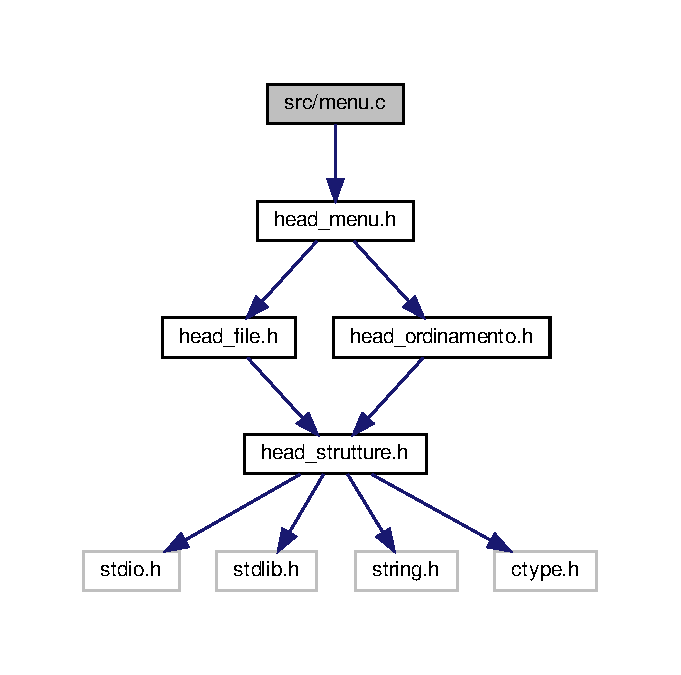
\includegraphics[width=327pt]{menu_8c__incl}
\end{center}
\end{figure}
\subsection*{Macros}
\begin{DoxyCompactItemize}
\item 
\#define \hyperlink{menu_8c_a4e6351c97432570c42e4bc1c36142400}{C\+H\+I\+U\+DI}~-\/1
\begin{DoxyCompactList}\small\item\em Definisce il valore che verra\textquotesingle{} considerato come quello per uscire. \end{DoxyCompactList}\end{DoxyCompactItemize}
\subsection*{Functions}
\begin{DoxyCompactItemize}
\item 
void \hyperlink{menu_8c_aa510a50efd9498c295969cf173fc6337}{show\+\_\+nolog\+\_\+menu} ()
\begin{DoxyCompactList}\small\item\em Mostra l\textquotesingle{}interfaccia grafica del menu\textquotesingle{} nolog. \end{DoxyCompactList}\item 
void \hyperlink{menu_8c_a0c94e4af9357a56b13dc6cf246a8fb92}{show\+\_\+log\+\_\+menu} ()
\begin{DoxyCompactList}\small\item\em Mostra l\textquotesingle{}interfaccia grafica del menu\textquotesingle{} log. \end{DoxyCompactList}\item 
void \hyperlink{menu_8c_a4f9be92c193bf45a9635e3c00bddc030}{show\+\_\+novita\+\_\+menu} ()
\begin{DoxyCompactList}\small\item\em Mostra l\textquotesingle{}interfaccia grafica del menu\textquotesingle{} principale novita\textquotesingle{}. \end{DoxyCompactList}\item 
void \hyperlink{menu_8c_aad25e471acaffe14832ddc5437f41c6d}{show\+\_\+prodotti\+\_\+menu} ()
\begin{DoxyCompactList}\small\item\em Mostra l\textquotesingle{}interfaccia grafica del menu\textquotesingle{} principale prodotti. \end{DoxyCompactList}\item 
void \hyperlink{menu_8c_adecccf77072a3787432afbfc4d87c4d8}{show\+\_\+clienti\+\_\+menu} ()
\begin{DoxyCompactList}\small\item\em Mostra l\textquotesingle{}interfaccia grafica del menu\textquotesingle{} principale clienti. \end{DoxyCompactList}\item 
void \hyperlink{menu_8c_a92366c9bd30febe9b239551d133525f1}{show\+\_\+dipendenti\+\_\+menu} ()
\begin{DoxyCompactList}\small\item\em Mostra l\textquotesingle{}interfaccia grafica del menu\textquotesingle{} principale dipendenti. \end{DoxyCompactList}\item 
void \hyperlink{menu_8c_a6b162ea688a7c5a59e96e8177dfda86d}{show\+\_\+ordinamento\+\_\+prodotti\+\_\+menu} ()
\begin{DoxyCompactList}\small\item\em Mostra l\textquotesingle{}interfaccia grafica del menu\textquotesingle{} per la scelta del tipo di ordinamento per i prodotti. \end{DoxyCompactList}\item 
void \hyperlink{menu_8c_ac9b4d8c08fe2a2db50c306d3c150ca28}{show\+\_\+ordinamento\+\_\+persone\+\_\+menu} ()
\begin{DoxyCompactList}\small\item\em Mostra l\textquotesingle{}interfaccia grafica del menu\textquotesingle{} per la scelta del tipo di ordinamento per dipendenti e clienti. \end{DoxyCompactList}\item 
void \hyperlink{menu_8c_afaa16c2b36a1936671f280a3cb40ad29}{login} (\hyperlink{head__strutture_8h_a784ca7b7fa64cbb661eb0c903348c1ce}{sessione\+\_\+t} $\ast$se)
\begin{DoxyCompactList}\small\item\em Gestisce l\textquotesingle{}accesso di un dipendente. \end{DoxyCompactList}\item 
int \hyperlink{menu_8c_adceb36f3ebfff88ac2283e19d50c01a6}{choise} (\hyperlink{head__strutture_8h_a27938a0a874a833cfee26456c5d730b1}{menu\+\_\+t} m)
\begin{DoxyCompactList}\small\item\em In base a quale menu\textquotesingle{} e\textquotesingle{} stato appena visualizzato, gestisce l\textquotesingle{}immissione dei possibili input controllandone la consistenza col tipo di menu.~\newline
Ritorna la scelta consistente dell\textquotesingle{}utente. \end{DoxyCompactList}\item 
int \hyperlink{menu_8c_a96fb221481623d0f77e6fd1e6f7ad118}{menu\+\_\+nextmove} (\hyperlink{head__strutture_8h_a784ca7b7fa64cbb661eb0c903348c1ce}{sessione\+\_\+t} $\ast$se)
\begin{DoxyCompactList}\small\item\em Imposta la prossima azione del programma. \end{DoxyCompactList}\end{DoxyCompactItemize}


\subsection{Detailed Description}
Il file contiene metodi per i menu\textquotesingle{} come visualizzazione e inserimento scelta. 

\subsection{Macro Definition Documentation}
\mbox{\Hypertarget{menu_8c_a4e6351c97432570c42e4bc1c36142400}\label{menu_8c_a4e6351c97432570c42e4bc1c36142400}} 
\index{menu.\+c@{menu.\+c}!C\+H\+I\+U\+DI@{C\+H\+I\+U\+DI}}
\index{C\+H\+I\+U\+DI@{C\+H\+I\+U\+DI}!menu.\+c@{menu.\+c}}
\subsubsection{\texorpdfstring{C\+H\+I\+U\+DI}{CHIUDI}}
{\footnotesize\ttfamily \#define C\+H\+I\+U\+DI~-\/1}



Definisce il valore che verra\textquotesingle{} considerato come quello per uscire. 



\subsection{Function Documentation}
\mbox{\Hypertarget{menu_8c_adceb36f3ebfff88ac2283e19d50c01a6}\label{menu_8c_adceb36f3ebfff88ac2283e19d50c01a6}} 
\index{menu.\+c@{menu.\+c}!choise@{choise}}
\index{choise@{choise}!menu.\+c@{menu.\+c}}
\subsubsection{\texorpdfstring{choise()}{choise()}}
{\footnotesize\ttfamily int choise (\begin{DoxyParamCaption}\item[{\hyperlink{head__strutture_8h_a27938a0a874a833cfee26456c5d730b1}{menu\+\_\+t}}]{m }\end{DoxyParamCaption})}



In base a quale menu\textquotesingle{} e\textquotesingle{} stato appena visualizzato, gestisce l\textquotesingle{}immissione dei possibili input controllandone la consistenza col tipo di menu.~\newline
Ritorna la scelta consistente dell\textquotesingle{}utente. 


\begin{DoxyParams}{Parameters}
{\em menu\+\_\+t} & menu \\
\hline
\end{DoxyParams}
\begin{DoxyReturn}{Returns}
int 
\end{DoxyReturn}
\mbox{\Hypertarget{menu_8c_afaa16c2b36a1936671f280a3cb40ad29}\label{menu_8c_afaa16c2b36a1936671f280a3cb40ad29}} 
\index{menu.\+c@{menu.\+c}!login@{login}}
\index{login@{login}!menu.\+c@{menu.\+c}}
\subsubsection{\texorpdfstring{login()}{login()}}
{\footnotesize\ttfamily void login (\begin{DoxyParamCaption}\item[{\hyperlink{head__strutture_8h_a784ca7b7fa64cbb661eb0c903348c1ce}{sessione\+\_\+t} $\ast$}]{se }\end{DoxyParamCaption})}



Gestisce l\textquotesingle{}accesso di un dipendente. 


\begin{DoxyParams}{Parameters}
{\em session\+\_\+t} & $\ast$sessione \\
\hline
\end{DoxyParams}
\mbox{\Hypertarget{menu_8c_a96fb221481623d0f77e6fd1e6f7ad118}\label{menu_8c_a96fb221481623d0f77e6fd1e6f7ad118}} 
\index{menu.\+c@{menu.\+c}!menu\+\_\+nextmove@{menu\+\_\+nextmove}}
\index{menu\+\_\+nextmove@{menu\+\_\+nextmove}!menu.\+c@{menu.\+c}}
\subsubsection{\texorpdfstring{menu\+\_\+nextmove()}{menu\_nextmove()}}
{\footnotesize\ttfamily int menu\+\_\+nextmove (\begin{DoxyParamCaption}\item[{\hyperlink{head__strutture_8h_a784ca7b7fa64cbb661eb0c903348c1ce}{sessione\+\_\+t} $\ast$}]{se }\end{DoxyParamCaption})}



Imposta la prossima azione del programma. 

In base alla scelta presente all\textquotesingle{}interno della sessione richiama i metodi necessari per la visualizzazione e il comportamento del menu\textquotesingle{} scelto, impostando i parametri della sessione se necessario.~\newline
Ritorna C\+H\+I\+U\+DI se e\textquotesingle{} la scelta in sessione era un chiudi, altrimenti ritorna 0. 
\begin{DoxyParams}{Parameters}
{\em sessione\+\_\+t} & $\ast$se \\
\hline
\end{DoxyParams}
\begin{DoxyReturn}{Returns}
int 
\end{DoxyReturn}
\mbox{\Hypertarget{menu_8c_adecccf77072a3787432afbfc4d87c4d8}\label{menu_8c_adecccf77072a3787432afbfc4d87c4d8}} 
\index{menu.\+c@{menu.\+c}!show\+\_\+clienti\+\_\+menu@{show\+\_\+clienti\+\_\+menu}}
\index{show\+\_\+clienti\+\_\+menu@{show\+\_\+clienti\+\_\+menu}!menu.\+c@{menu.\+c}}
\subsubsection{\texorpdfstring{show\+\_\+clienti\+\_\+menu()}{show\_clienti\_menu()}}
{\footnotesize\ttfamily void show\+\_\+clienti\+\_\+menu (\begin{DoxyParamCaption}{ }\end{DoxyParamCaption})}



Mostra l\textquotesingle{}interfaccia grafica del menu\textquotesingle{} principale clienti. 

\mbox{\Hypertarget{menu_8c_a92366c9bd30febe9b239551d133525f1}\label{menu_8c_a92366c9bd30febe9b239551d133525f1}} 
\index{menu.\+c@{menu.\+c}!show\+\_\+dipendenti\+\_\+menu@{show\+\_\+dipendenti\+\_\+menu}}
\index{show\+\_\+dipendenti\+\_\+menu@{show\+\_\+dipendenti\+\_\+menu}!menu.\+c@{menu.\+c}}
\subsubsection{\texorpdfstring{show\+\_\+dipendenti\+\_\+menu()}{show\_dipendenti\_menu()}}
{\footnotesize\ttfamily void show\+\_\+dipendenti\+\_\+menu (\begin{DoxyParamCaption}{ }\end{DoxyParamCaption})}



Mostra l\textquotesingle{}interfaccia grafica del menu\textquotesingle{} principale dipendenti. 

\mbox{\Hypertarget{menu_8c_a0c94e4af9357a56b13dc6cf246a8fb92}\label{menu_8c_a0c94e4af9357a56b13dc6cf246a8fb92}} 
\index{menu.\+c@{menu.\+c}!show\+\_\+log\+\_\+menu@{show\+\_\+log\+\_\+menu}}
\index{show\+\_\+log\+\_\+menu@{show\+\_\+log\+\_\+menu}!menu.\+c@{menu.\+c}}
\subsubsection{\texorpdfstring{show\+\_\+log\+\_\+menu()}{show\_log\_menu()}}
{\footnotesize\ttfamily void show\+\_\+log\+\_\+menu (\begin{DoxyParamCaption}{ }\end{DoxyParamCaption})}



Mostra l\textquotesingle{}interfaccia grafica del menu\textquotesingle{} log. 

\mbox{\Hypertarget{menu_8c_aa510a50efd9498c295969cf173fc6337}\label{menu_8c_aa510a50efd9498c295969cf173fc6337}} 
\index{menu.\+c@{menu.\+c}!show\+\_\+nolog\+\_\+menu@{show\+\_\+nolog\+\_\+menu}}
\index{show\+\_\+nolog\+\_\+menu@{show\+\_\+nolog\+\_\+menu}!menu.\+c@{menu.\+c}}
\subsubsection{\texorpdfstring{show\+\_\+nolog\+\_\+menu()}{show\_nolog\_menu()}}
{\footnotesize\ttfamily void show\+\_\+nolog\+\_\+menu (\begin{DoxyParamCaption}{ }\end{DoxyParamCaption})}



Mostra l\textquotesingle{}interfaccia grafica del menu\textquotesingle{} nolog. 

\mbox{\Hypertarget{menu_8c_a4f9be92c193bf45a9635e3c00bddc030}\label{menu_8c_a4f9be92c193bf45a9635e3c00bddc030}} 
\index{menu.\+c@{menu.\+c}!show\+\_\+novita\+\_\+menu@{show\+\_\+novita\+\_\+menu}}
\index{show\+\_\+novita\+\_\+menu@{show\+\_\+novita\+\_\+menu}!menu.\+c@{menu.\+c}}
\subsubsection{\texorpdfstring{show\+\_\+novita\+\_\+menu()}{show\_novita\_menu()}}
{\footnotesize\ttfamily void show\+\_\+novita\+\_\+menu (\begin{DoxyParamCaption}{ }\end{DoxyParamCaption})}



Mostra l\textquotesingle{}interfaccia grafica del menu\textquotesingle{} principale novita\textquotesingle{}. 

\mbox{\Hypertarget{menu_8c_ac9b4d8c08fe2a2db50c306d3c150ca28}\label{menu_8c_ac9b4d8c08fe2a2db50c306d3c150ca28}} 
\index{menu.\+c@{menu.\+c}!show\+\_\+ordinamento\+\_\+persone\+\_\+menu@{show\+\_\+ordinamento\+\_\+persone\+\_\+menu}}
\index{show\+\_\+ordinamento\+\_\+persone\+\_\+menu@{show\+\_\+ordinamento\+\_\+persone\+\_\+menu}!menu.\+c@{menu.\+c}}
\subsubsection{\texorpdfstring{show\+\_\+ordinamento\+\_\+persone\+\_\+menu()}{show\_ordinamento\_persone\_menu()}}
{\footnotesize\ttfamily void show\+\_\+ordinamento\+\_\+persone\+\_\+menu (\begin{DoxyParamCaption}{ }\end{DoxyParamCaption})}



Mostra l\textquotesingle{}interfaccia grafica del menu\textquotesingle{} per la scelta del tipo di ordinamento per dipendenti e clienti. 

\mbox{\Hypertarget{menu_8c_a6b162ea688a7c5a59e96e8177dfda86d}\label{menu_8c_a6b162ea688a7c5a59e96e8177dfda86d}} 
\index{menu.\+c@{menu.\+c}!show\+\_\+ordinamento\+\_\+prodotti\+\_\+menu@{show\+\_\+ordinamento\+\_\+prodotti\+\_\+menu}}
\index{show\+\_\+ordinamento\+\_\+prodotti\+\_\+menu@{show\+\_\+ordinamento\+\_\+prodotti\+\_\+menu}!menu.\+c@{menu.\+c}}
\subsubsection{\texorpdfstring{show\+\_\+ordinamento\+\_\+prodotti\+\_\+menu()}{show\_ordinamento\_prodotti\_menu()}}
{\footnotesize\ttfamily void show\+\_\+ordinamento\+\_\+prodotti\+\_\+menu (\begin{DoxyParamCaption}{ }\end{DoxyParamCaption})}



Mostra l\textquotesingle{}interfaccia grafica del menu\textquotesingle{} per la scelta del tipo di ordinamento per i prodotti. 

\mbox{\Hypertarget{menu_8c_aad25e471acaffe14832ddc5437f41c6d}\label{menu_8c_aad25e471acaffe14832ddc5437f41c6d}} 
\index{menu.\+c@{menu.\+c}!show\+\_\+prodotti\+\_\+menu@{show\+\_\+prodotti\+\_\+menu}}
\index{show\+\_\+prodotti\+\_\+menu@{show\+\_\+prodotti\+\_\+menu}!menu.\+c@{menu.\+c}}
\subsubsection{\texorpdfstring{show\+\_\+prodotti\+\_\+menu()}{show\_prodotti\_menu()}}
{\footnotesize\ttfamily void show\+\_\+prodotti\+\_\+menu (\begin{DoxyParamCaption}{ }\end{DoxyParamCaption})}



Mostra l\textquotesingle{}interfaccia grafica del menu\textquotesingle{} principale prodotti. 


\hypertarget{ordinamento_8c}{}\section{src/ordinamento.c File Reference}
\label{ordinamento_8c}\index{src/ordinamento.\+c@{src/ordinamento.\+c}}
{\ttfamily \#include \char`\"{}head\+\_\+ordinamento.\+h\char`\"{}}\newline
Include dependency graph for ordinamento.\+c\+:
\nopagebreak
\begin{figure}[H]
\begin{center}
\leavevmode
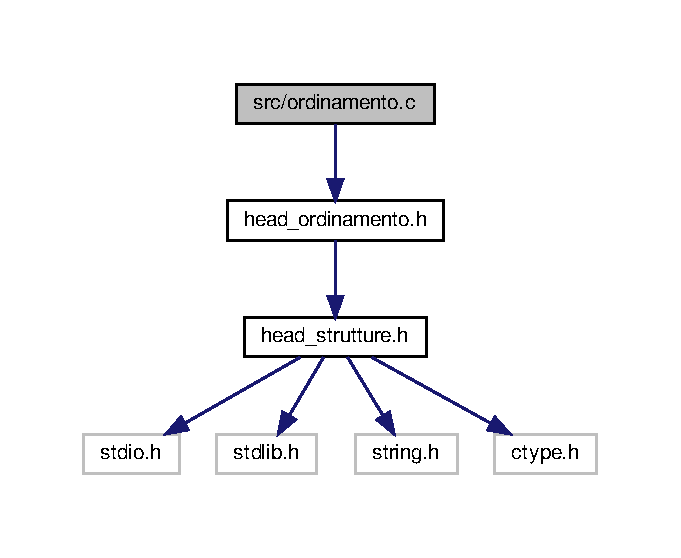
\includegraphics[width=327pt]{ordinamento_8c__incl}
\end{center}
\end{figure}
\subsection*{Functions}
\begin{DoxyCompactItemize}
\item 
void \hyperlink{ordinamento_8c_a3bc01b8dc1cfe1be1a3c7ac22af0c183}{destroy\+\_\+tree} (\hyperlink{head__strutture_8h_a4ef1b6d5b50a013be973ef01962dc932}{tree\+\_\+node\+\_\+t} $\ast$n)
\begin{DoxyCompactList}\small\item\em Libera la memoria allocata dell\textquotesingle{}albero a partire dal nodo passato come parametro. \end{DoxyCompactList}\item 
void \hyperlink{ordinamento_8c_a3ee60e03d675a4b6c5f3e23b126142cd}{insert\+\_\+key\+\_\+prodotti} (\hyperlink{head__strutture_8h_afec16ee1fceb6c05f4be3538f36b1997}{prodotto\+\_\+t} $\ast$record, \hyperlink{head__strutture_8h_a4ef1b6d5b50a013be973ef01962dc932}{tree\+\_\+node\+\_\+t} $\ast$$\ast$n, \hyperlink{head__strutture_8h_a3da5d27de6c586fecb3c1412cc6f1265}{campo\+\_\+record\+\_\+t} campo)
\begin{DoxyCompactList}\small\item\em Inserisce il record nella posizione giusta dell\textquotesingle{}albero, la cui radice e\textquotesingle{} il nodo passato come parametro. \end{DoxyCompactList}\item 
void \hyperlink{ordinamento_8c_a106d61401ba95025e29d6726736c03de}{insert\+\_\+key\+\_\+persone} (\hyperlink{head__strutture_8h_a58439881922e3f6e7ed51e352f2a0c1c}{persona\+\_\+t} $\ast$record, \hyperlink{head__strutture_8h_a4ef1b6d5b50a013be973ef01962dc932}{tree\+\_\+node\+\_\+t} $\ast$$\ast$n, \hyperlink{head__strutture_8h_a3da5d27de6c586fecb3c1412cc6f1265}{campo\+\_\+record\+\_\+t} campo)
\begin{DoxyCompactList}\small\item\em Inserisce il record nella posizione giusta dell\textquotesingle{}albero, la cui radice e\textquotesingle{} il nodo passato come parametro. \end{DoxyCompactList}\item 
void \hyperlink{ordinamento_8c_a6bdfab8e39d9f55f2213b9ecffddf816}{print\+\_\+tree} (\hyperlink{head__strutture_8h_a4ef1b6d5b50a013be973ef01962dc932}{tree\+\_\+node\+\_\+t} $\ast$$\ast$n, \hyperlink{head__strutture_8h_ad83512da590021d7b336c3cb314dc228}{tipofile\+\_\+t} tipo)
\begin{DoxyCompactList}\small\item\em Stampa l\textquotesingle{}albero a partire dal nodo passato come parametro, e\textquotesingle{} necessario specificare il tipo file che si usera\textquotesingle{}. \end{DoxyCompactList}\item 
void \hyperlink{ordinamento_8c_a18de588a8118a4cbda403d11b1dbaf16}{print\+\_\+file} (\hyperlink{head__strutture_8h_ad83512da590021d7b336c3cb314dc228}{tipofile\+\_\+t} tipo, \hyperlink{head__strutture_8h_a3da5d27de6c586fecb3c1412cc6f1265}{campo\+\_\+record\+\_\+t} campo)
\begin{DoxyCompactList}\small\item\em Stampa l\textquotesingle{}intero file selezionato datl tipo file passato come parametro, ordinato a seconda del campo passato come parametro. \end{DoxyCompactList}\end{DoxyCompactItemize}


\subsection{Detailed Description}
Contiene i metodi inerenti alla creazione di un albero binario ordinato, e alla visualizzazione di esso. 

\subsection{Function Documentation}
\mbox{\Hypertarget{ordinamento_8c_a3bc01b8dc1cfe1be1a3c7ac22af0c183}\label{ordinamento_8c_a3bc01b8dc1cfe1be1a3c7ac22af0c183}} 
\index{ordinamento.\+c@{ordinamento.\+c}!destroy\+\_\+tree@{destroy\+\_\+tree}}
\index{destroy\+\_\+tree@{destroy\+\_\+tree}!ordinamento.\+c@{ordinamento.\+c}}
\subsubsection{\texorpdfstring{destroy\+\_\+tree()}{destroy\_tree()}}
{\footnotesize\ttfamily void destroy\+\_\+tree (\begin{DoxyParamCaption}\item[{\hyperlink{head__strutture_8h_a4ef1b6d5b50a013be973ef01962dc932}{tree\+\_\+node\+\_\+t} $\ast$}]{n }\end{DoxyParamCaption})}



Libera la memoria allocata dell\textquotesingle{}albero a partire dal nodo passato come parametro. 

Se viene passata la radice, tutta la memoria allocata delll\textquotesingle{}albero verra\textquotesingle{} liberata. 
\begin{DoxyParams}{Parameters}
{\em tree\+\_\+node\+\_\+t} & $\ast$ nodo \\
\hline
\end{DoxyParams}
\mbox{\Hypertarget{ordinamento_8c_a106d61401ba95025e29d6726736c03de}\label{ordinamento_8c_a106d61401ba95025e29d6726736c03de}} 
\index{ordinamento.\+c@{ordinamento.\+c}!insert\+\_\+key\+\_\+persone@{insert\+\_\+key\+\_\+persone}}
\index{insert\+\_\+key\+\_\+persone@{insert\+\_\+key\+\_\+persone}!ordinamento.\+c@{ordinamento.\+c}}
\subsubsection{\texorpdfstring{insert\+\_\+key\+\_\+persone()}{insert\_key\_persone()}}
{\footnotesize\ttfamily void insert\+\_\+key\+\_\+persone (\begin{DoxyParamCaption}\item[{\hyperlink{head__strutture_8h_a58439881922e3f6e7ed51e352f2a0c1c}{persona\+\_\+t} $\ast$}]{record,  }\item[{\hyperlink{head__strutture_8h_a4ef1b6d5b50a013be973ef01962dc932}{tree\+\_\+node\+\_\+t} $\ast$$\ast$}]{n,  }\item[{\hyperlink{head__strutture_8h_a3da5d27de6c586fecb3c1412cc6f1265}{campo\+\_\+record\+\_\+t}}]{campo }\end{DoxyParamCaption})}



Inserisce il record nella posizione giusta dell\textquotesingle{}albero, la cui radice e\textquotesingle{} il nodo passato come parametro. 

E\textquotesingle{} possibile sceglire il campo da considerare per l\textquotesingle{}ordinamento. 
\begin{DoxyParams}{Parameters}
{\em persona\+\_\+t} & $\ast$record \\
\hline
{\em tree\+\_\+node\+\_\+t} & $\ast$$\ast$radice \\
\hline
{\em campo\+\_\+record\+\_\+t} & campo \\
\hline
\end{DoxyParams}
\mbox{\Hypertarget{ordinamento_8c_a3ee60e03d675a4b6c5f3e23b126142cd}\label{ordinamento_8c_a3ee60e03d675a4b6c5f3e23b126142cd}} 
\index{ordinamento.\+c@{ordinamento.\+c}!insert\+\_\+key\+\_\+prodotti@{insert\+\_\+key\+\_\+prodotti}}
\index{insert\+\_\+key\+\_\+prodotti@{insert\+\_\+key\+\_\+prodotti}!ordinamento.\+c@{ordinamento.\+c}}
\subsubsection{\texorpdfstring{insert\+\_\+key\+\_\+prodotti()}{insert\_key\_prodotti()}}
{\footnotesize\ttfamily void insert\+\_\+key\+\_\+prodotti (\begin{DoxyParamCaption}\item[{\hyperlink{head__strutture_8h_afec16ee1fceb6c05f4be3538f36b1997}{prodotto\+\_\+t} $\ast$}]{record,  }\item[{\hyperlink{head__strutture_8h_a4ef1b6d5b50a013be973ef01962dc932}{tree\+\_\+node\+\_\+t} $\ast$$\ast$}]{n,  }\item[{\hyperlink{head__strutture_8h_a3da5d27de6c586fecb3c1412cc6f1265}{campo\+\_\+record\+\_\+t}}]{campo }\end{DoxyParamCaption})}



Inserisce il record nella posizione giusta dell\textquotesingle{}albero, la cui radice e\textquotesingle{} il nodo passato come parametro. 

E\textquotesingle{} possibile sceglire il campo da considerare per l\textquotesingle{}ordinamento. 
\begin{DoxyParams}{Parameters}
{\em prodotto\+\_\+t} & $\ast$record \\
\hline
{\em tree\+\_\+node\+\_\+t} & $\ast$$\ast$radice \\
\hline
{\em campo\+\_\+record\+\_\+t} & campo \\
\hline
\end{DoxyParams}
\begin{DoxyRefDesc}{Bug}
\item[\hyperlink{bug__bug000001}{Bug}]L\textquotesingle{}ordinamento alfabetico funziona cosi\textquotesingle{} per ora\+: ordinamento alfabetico sulla prima lettera del nome e se uguale mette prima quello con id minore (si sa\textquotesingle{} il perche\textquotesingle{}) \end{DoxyRefDesc}
\mbox{\Hypertarget{ordinamento_8c_a18de588a8118a4cbda403d11b1dbaf16}\label{ordinamento_8c_a18de588a8118a4cbda403d11b1dbaf16}} 
\index{ordinamento.\+c@{ordinamento.\+c}!print\+\_\+file@{print\+\_\+file}}
\index{print\+\_\+file@{print\+\_\+file}!ordinamento.\+c@{ordinamento.\+c}}
\subsubsection{\texorpdfstring{print\+\_\+file()}{print\_file()}}
{\footnotesize\ttfamily void print\+\_\+file (\begin{DoxyParamCaption}\item[{\hyperlink{head__strutture_8h_ad83512da590021d7b336c3cb314dc228}{tipofile\+\_\+t}}]{tipo,  }\item[{\hyperlink{head__strutture_8h_a3da5d27de6c586fecb3c1412cc6f1265}{campo\+\_\+record\+\_\+t}}]{campo }\end{DoxyParamCaption})}



Stampa l\textquotesingle{}intero file selezionato datl tipo file passato come parametro, ordinato a seconda del campo passato come parametro. 


\begin{DoxyParams}{Parameters}
{\em tipofile\+\_\+t} & tipo \\
\hline
{\em campo\+\_\+record\+\_\+t} & campo \\
\hline
\end{DoxyParams}
\mbox{\Hypertarget{ordinamento_8c_a6bdfab8e39d9f55f2213b9ecffddf816}\label{ordinamento_8c_a6bdfab8e39d9f55f2213b9ecffddf816}} 
\index{ordinamento.\+c@{ordinamento.\+c}!print\+\_\+tree@{print\+\_\+tree}}
\index{print\+\_\+tree@{print\+\_\+tree}!ordinamento.\+c@{ordinamento.\+c}}
\subsubsection{\texorpdfstring{print\+\_\+tree()}{print\_tree()}}
{\footnotesize\ttfamily void print\+\_\+tree (\begin{DoxyParamCaption}\item[{\hyperlink{head__strutture_8h_a4ef1b6d5b50a013be973ef01962dc932}{tree\+\_\+node\+\_\+t} $\ast$$\ast$}]{n,  }\item[{\hyperlink{head__strutture_8h_ad83512da590021d7b336c3cb314dc228}{tipofile\+\_\+t}}]{tipo }\end{DoxyParamCaption})}



Stampa l\textquotesingle{}albero a partire dal nodo passato come parametro, e\textquotesingle{} necessario specificare il tipo file che si usera\textquotesingle{}. 


\begin{DoxyParams}{Parameters}
{\em tree\+\_\+node\+\_\+t} & $\ast$$\ast$nodo \\
\hline
{\em tipofile\+\_\+t} & tipo \\
\hline
\end{DoxyParams}

\hypertarget{strutture_8c}{}\section{src/strutture.c File Reference}
\label{strutture_8c}\index{src/strutture.\+c@{src/strutture.\+c}}
{\ttfamily \#include \char`\"{}head\+\_\+strutture.\+h\char`\"{}}\newline
Include dependency graph for strutture.\+c\+:
\nopagebreak
\begin{figure}[H]
\begin{center}
\leavevmode
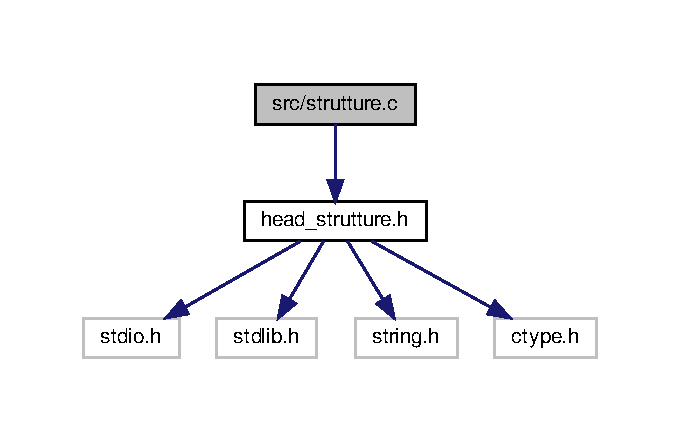
\includegraphics[width=327pt]{strutture_8c__incl}
\end{center}
\end{figure}
\subsection*{Functions}
\begin{DoxyCompactItemize}
\item 
void \hyperlink{strutture_8c_af2763b0dcb4f38febe8620bb4f65736d}{initialize\+\_\+session} (\hyperlink{head__strutture_8h_a784ca7b7fa64cbb661eb0c903348c1ce}{sessione\+\_\+t} $\ast$se)
\begin{DoxyCompactList}\small\item\em Inizializza le componenti di una struttura sessione. \end{DoxyCompactList}\item 
void \hyperlink{strutture_8c_ae517940db604a664f340a08b4c1b1ee3}{initialize\+\_\+prodotto} (\hyperlink{head__strutture_8h_afec16ee1fceb6c05f4be3538f36b1997}{prodotto\+\_\+t} $\ast$p)
\begin{DoxyCompactList}\small\item\em Inizializza le componenti di una struttura prodotto. \end{DoxyCompactList}\item 
void \hyperlink{strutture_8c_a973195d321eed8af362eac78b711fd0f}{initialize\+\_\+persona} (\hyperlink{head__strutture_8h_a58439881922e3f6e7ed51e352f2a0c1c}{persona\+\_\+t} $\ast$p)
\begin{DoxyCompactList}\small\item\em Inizializza le componenti di una struttura persona. \end{DoxyCompactList}\item 
void \hyperlink{strutture_8c_a8f08cdbfd563b68a75bef38e80c16cbc}{get\+\_\+prodotto} (\hyperlink{head__strutture_8h_afec16ee1fceb6c05f4be3538f36b1997}{prodotto\+\_\+t} $\ast$\hyperlink{structprodotto}{prodotto}, F\+I\+LE $\ast$fp)
\begin{DoxyCompactList}\small\item\em Carica in prodotto i dati di una riga del file prodotti.\+txt. \end{DoxyCompactList}\item 
void \hyperlink{strutture_8c_a4717013d0abaa8c175dafda3925c3931}{get\+\_\+persona} (\hyperlink{head__strutture_8h_a58439881922e3f6e7ed51e352f2a0c1c}{persona\+\_\+t} $\ast$\hyperlink{structpersona}{persona}, F\+I\+LE $\ast$fp)
\begin{DoxyCompactList}\small\item\em Carica in persona i dati di una riga del file clienti.\+txt o dipendenti.\+txt. \end{DoxyCompactList}\item 
void \hyperlink{strutture_8c_ad95b3b50d33dc0d99ce72e61aefe65e6}{get\+\_\+string} (char $\ast$stringa, int lunghezza)
\begin{DoxyCompactList}\small\item\em Estrae da stdin una stringa di lunghezza massima data e la mette nella stringa passata come parametro, pone sempre \textbackslash{}0 alla fine. \end{DoxyCompactList}\item 
void \hyperlink{strutture_8c_ac85ae6df551b530c1638d7ebc48ab48a}{get\+\_\+string\+\_\+file} (char $\ast$stringa, int lunghezza, F\+I\+LE $\ast$fp)
\begin{DoxyCompactList}\small\item\em Estrae dal file passato come parametro una stringa di lunghezza massima data e la mette nella stringa passata come parametro, pone sempre \textbackslash{}0 alla fine. \end{DoxyCompactList}\item 
int \hyperlink{strutture_8c_ac472caf5ab5d1500de32eb9389419a0d}{is\+\_\+unum} (char $\ast$stringa)
\begin{DoxyCompactList}\small\item\em Controlla se la stringa passata come parametro contiene solo caratteri numerici interi senza segno. \end{DoxyCompactList}\item 
int \hyperlink{strutture_8c_a80d803c9093f8a72403d83adbaee7c42}{is\+\_\+num} (char $\ast$stringa)
\begin{DoxyCompactList}\small\item\em Controlla se la stringa passata come parametro contiene solo caratteri numerici interi con segno. \end{DoxyCompactList}\item 
int \hyperlink{strutture_8c_ad112c9780a37fb8cd6c53e0475fbdc3c}{is\+\_\+ufnum} (char $\ast$stringa)
\begin{DoxyCompactList}\small\item\em Controlla se la stringa passata come parametro contiene solo caratteri numerici interi o non senza segno. \end{DoxyCompactList}\end{DoxyCompactItemize}


\subsection{Detailed Description}
Contiene i metodi inerenti alle strutture e altri metodi utili come\+:~\newline
-\/)Inizializzazione delle variabili che compongono una struttura.~\newline
-\/)Controlli di consistenza di un tipo di dato.~\newline
-\/)Gestione d\textquotesingle{}ellimput di stringhe da stdin e non. 

\subsection{Function Documentation}
\mbox{\Hypertarget{strutture_8c_a4717013d0abaa8c175dafda3925c3931}\label{strutture_8c_a4717013d0abaa8c175dafda3925c3931}} 
\index{strutture.\+c@{strutture.\+c}!get\+\_\+persona@{get\+\_\+persona}}
\index{get\+\_\+persona@{get\+\_\+persona}!strutture.\+c@{strutture.\+c}}
\subsubsection{\texorpdfstring{get\+\_\+persona()}{get\_persona()}}
{\footnotesize\ttfamily void get\+\_\+persona (\begin{DoxyParamCaption}\item[{\hyperlink{head__strutture_8h_a58439881922e3f6e7ed51e352f2a0c1c}{persona\+\_\+t} $\ast$}]{persona,  }\item[{F\+I\+LE $\ast$}]{fp }\end{DoxyParamCaption})}



Carica in persona i dati di una riga del file clienti.\+txt o dipendenti.\+txt. 

Si ipotizza di essere nella posizione giusta e che il puntatore al file sia open.~\newline
Alla fine lascia il puntatore sulla nuova riga se esiste. 
\begin{DoxyParams}{Parameters}
{\em persona\+\_\+t} & $\ast$persona \\
\hline
{\em F\+I\+LE} & $\ast$file \\
\hline
\end{DoxyParams}
\mbox{\Hypertarget{strutture_8c_a8f08cdbfd563b68a75bef38e80c16cbc}\label{strutture_8c_a8f08cdbfd563b68a75bef38e80c16cbc}} 
\index{strutture.\+c@{strutture.\+c}!get\+\_\+prodotto@{get\+\_\+prodotto}}
\index{get\+\_\+prodotto@{get\+\_\+prodotto}!strutture.\+c@{strutture.\+c}}
\subsubsection{\texorpdfstring{get\+\_\+prodotto()}{get\_prodotto()}}
{\footnotesize\ttfamily void get\+\_\+prodotto (\begin{DoxyParamCaption}\item[{\hyperlink{head__strutture_8h_afec16ee1fceb6c05f4be3538f36b1997}{prodotto\+\_\+t} $\ast$}]{prodotto,  }\item[{F\+I\+LE $\ast$}]{fp }\end{DoxyParamCaption})}



Carica in prodotto i dati di una riga del file prodotti.\+txt. 

Si ipotizza di essere nella posizione giusta e che il puntatore al file sia open.~\newline
Alla fine lascia il puntatore sulla nuova riga se esiste. 
\begin{DoxyParams}{Parameters}
{\em prodotto\+\_\+t} & $\ast$prodotto \\
\hline
{\em F\+I\+LE} & $\ast$file \\
\hline
\end{DoxyParams}
\mbox{\Hypertarget{strutture_8c_ad95b3b50d33dc0d99ce72e61aefe65e6}\label{strutture_8c_ad95b3b50d33dc0d99ce72e61aefe65e6}} 
\index{strutture.\+c@{strutture.\+c}!get\+\_\+string@{get\+\_\+string}}
\index{get\+\_\+string@{get\+\_\+string}!strutture.\+c@{strutture.\+c}}
\subsubsection{\texorpdfstring{get\+\_\+string()}{get\_string()}}
{\footnotesize\ttfamily void get\+\_\+string (\begin{DoxyParamCaption}\item[{char $\ast$}]{stringa,  }\item[{int}]{lunghezza }\end{DoxyParamCaption})}



Estrae da stdin una stringa di lunghezza massima data e la mette nella stringa passata come parametro, pone sempre \textbackslash{}0 alla fine. 

Se ci sono piu\textquotesingle{} caratteri di quelli ammissibili svuota anche il buffer. 
\begin{DoxyParams}{Parameters}
{\em char} & $\ast$stringa \\
\hline
{\em int} & lunghezza \\
\hline
\end{DoxyParams}
\mbox{\Hypertarget{strutture_8c_ac85ae6df551b530c1638d7ebc48ab48a}\label{strutture_8c_ac85ae6df551b530c1638d7ebc48ab48a}} 
\index{strutture.\+c@{strutture.\+c}!get\+\_\+string\+\_\+file@{get\+\_\+string\+\_\+file}}
\index{get\+\_\+string\+\_\+file@{get\+\_\+string\+\_\+file}!strutture.\+c@{strutture.\+c}}
\subsubsection{\texorpdfstring{get\+\_\+string\+\_\+file()}{get\_string\_file()}}
{\footnotesize\ttfamily void get\+\_\+string\+\_\+file (\begin{DoxyParamCaption}\item[{char $\ast$}]{stringa,  }\item[{int}]{lunghezza,  }\item[{F\+I\+LE $\ast$}]{fp }\end{DoxyParamCaption})}



Estrae dal file passato come parametro una stringa di lunghezza massima data e la mette nella stringa passata come parametro, pone sempre \textbackslash{}0 alla fine. 

Se ci sono piu\textquotesingle{} caratteri di quelli ammissibili svuota anche il buffer. A\+T\+T\+E\+N\+Z\+I\+O\+NE\+: Questo metodo non e\textquotesingle{} mai stato utilizzato nel programma quindi potrebbe non funzionare correttamente, potrebbe tornare utile. 
\begin{DoxyParams}{Parameters}
{\em char} & $\ast$stringa \\
\hline
{\em int} & lunghezza \\
\hline
{\em F\+I\+LE} & $\ast$fp \\
\hline
\end{DoxyParams}
\mbox{\Hypertarget{strutture_8c_a973195d321eed8af362eac78b711fd0f}\label{strutture_8c_a973195d321eed8af362eac78b711fd0f}} 
\index{strutture.\+c@{strutture.\+c}!initialize\+\_\+persona@{initialize\+\_\+persona}}
\index{initialize\+\_\+persona@{initialize\+\_\+persona}!strutture.\+c@{strutture.\+c}}
\subsubsection{\texorpdfstring{initialize\+\_\+persona()}{initialize\_persona()}}
{\footnotesize\ttfamily void initialize\+\_\+persona (\begin{DoxyParamCaption}\item[{\hyperlink{head__strutture_8h_a58439881922e3f6e7ed51e352f2a0c1c}{persona\+\_\+t} $\ast$}]{p }\end{DoxyParamCaption})}



Inizializza le componenti di una struttura persona. 


\begin{DoxyParams}{Parameters}
{\em persona\+\_\+t} & $\ast$persona \\
\hline
\end{DoxyParams}
\mbox{\Hypertarget{strutture_8c_ae517940db604a664f340a08b4c1b1ee3}\label{strutture_8c_ae517940db604a664f340a08b4c1b1ee3}} 
\index{strutture.\+c@{strutture.\+c}!initialize\+\_\+prodotto@{initialize\+\_\+prodotto}}
\index{initialize\+\_\+prodotto@{initialize\+\_\+prodotto}!strutture.\+c@{strutture.\+c}}
\subsubsection{\texorpdfstring{initialize\+\_\+prodotto()}{initialize\_prodotto()}}
{\footnotesize\ttfamily void initialize\+\_\+prodotto (\begin{DoxyParamCaption}\item[{\hyperlink{head__strutture_8h_afec16ee1fceb6c05f4be3538f36b1997}{prodotto\+\_\+t} $\ast$}]{p }\end{DoxyParamCaption})}



Inizializza le componenti di una struttura prodotto. 


\begin{DoxyParams}{Parameters}
{\em prodotto\+\_\+t} & $\ast$prodotto \\
\hline
\end{DoxyParams}
\mbox{\Hypertarget{strutture_8c_af2763b0dcb4f38febe8620bb4f65736d}\label{strutture_8c_af2763b0dcb4f38febe8620bb4f65736d}} 
\index{strutture.\+c@{strutture.\+c}!initialize\+\_\+session@{initialize\+\_\+session}}
\index{initialize\+\_\+session@{initialize\+\_\+session}!strutture.\+c@{strutture.\+c}}
\subsubsection{\texorpdfstring{initialize\+\_\+session()}{initialize\_session()}}
{\footnotesize\ttfamily void initialize\+\_\+session (\begin{DoxyParamCaption}\item[{\hyperlink{head__strutture_8h_a784ca7b7fa64cbb661eb0c903348c1ce}{sessione\+\_\+t} $\ast$}]{se }\end{DoxyParamCaption})}



Inizializza le componenti di una struttura sessione. 


\begin{DoxyParams}{Parameters}
{\em sessione\+\_\+t} & $\ast$sessione \\
\hline
\end{DoxyParams}
\mbox{\Hypertarget{strutture_8c_a80d803c9093f8a72403d83adbaee7c42}\label{strutture_8c_a80d803c9093f8a72403d83adbaee7c42}} 
\index{strutture.\+c@{strutture.\+c}!is\+\_\+num@{is\+\_\+num}}
\index{is\+\_\+num@{is\+\_\+num}!strutture.\+c@{strutture.\+c}}
\subsubsection{\texorpdfstring{is\+\_\+num()}{is\_num()}}
{\footnotesize\ttfamily int is\+\_\+num (\begin{DoxyParamCaption}\item[{char $\ast$}]{stringa }\end{DoxyParamCaption})}



Controlla se la stringa passata come parametro contiene solo caratteri numerici interi con segno. 

Ritorna 0 se la stringa corrisponde al tipo definito, -\/1 altrimenti. 
\begin{DoxyParams}{Parameters}
{\em char} & $\ast$stringa \\
\hline
\end{DoxyParams}
\begin{DoxyReturn}{Returns}
int 
\end{DoxyReturn}
\mbox{\Hypertarget{strutture_8c_ad112c9780a37fb8cd6c53e0475fbdc3c}\label{strutture_8c_ad112c9780a37fb8cd6c53e0475fbdc3c}} 
\index{strutture.\+c@{strutture.\+c}!is\+\_\+ufnum@{is\+\_\+ufnum}}
\index{is\+\_\+ufnum@{is\+\_\+ufnum}!strutture.\+c@{strutture.\+c}}
\subsubsection{\texorpdfstring{is\+\_\+ufnum()}{is\_ufnum()}}
{\footnotesize\ttfamily int is\+\_\+ufnum (\begin{DoxyParamCaption}\item[{char $\ast$}]{stringa }\end{DoxyParamCaption})}



Controlla se la stringa passata come parametro contiene solo caratteri numerici interi o non senza segno. 

Ritorna 0 se la stringa corrisponde al tipo definito, -\/1 altrimenti. 
\begin{DoxyParams}{Parameters}
{\em char} & $\ast$stringa \\
\hline
\end{DoxyParams}
\begin{DoxyReturn}{Returns}
int 
\end{DoxyReturn}
\begin{DoxyRefDesc}{Bug}
\item[\hyperlink{bug__bug000002}{Bug}]E\textquotesingle{} stato necessario includere sia , che . quindi potrebbe avere un comportamento leggermente diverso se usato un delimitatore di cifre diverso da quello definito dal proprio sistema (non causa comunque errori gravi, si perde al massimo la parte decimale). \end{DoxyRefDesc}
\mbox{\Hypertarget{strutture_8c_ac472caf5ab5d1500de32eb9389419a0d}\label{strutture_8c_ac472caf5ab5d1500de32eb9389419a0d}} 
\index{strutture.\+c@{strutture.\+c}!is\+\_\+unum@{is\+\_\+unum}}
\index{is\+\_\+unum@{is\+\_\+unum}!strutture.\+c@{strutture.\+c}}
\subsubsection{\texorpdfstring{is\+\_\+unum()}{is\_unum()}}
{\footnotesize\ttfamily int is\+\_\+unum (\begin{DoxyParamCaption}\item[{char $\ast$}]{stringa }\end{DoxyParamCaption})}



Controlla se la stringa passata come parametro contiene solo caratteri numerici interi senza segno. 

Ritorna 0 se la stringa corrisponde al tipo definito, -\/1 altrimenti. 
\begin{DoxyParams}{Parameters}
{\em char} & $\ast$stringa \\
\hline
\end{DoxyParams}
\begin{DoxyReturn}{Returns}
int 
\end{DoxyReturn}

%--- End generated contents ---

% Index
\backmatter
\newpage
\phantomsection
\clearemptydoublepage
\addcontentsline{toc}{chapter}{Index}
\printindex

\end{document}
